\section{Numerical examples}
\label{section: Chapter3/examples}

%%%%%%%%%%%%%%%%%%%%%%%%%%%%%%%%%%%%%%%%%%%%%%%%%%%%%%%%%%%%%%%%%%%%%%%%%%%%%%%%%%%%%%%%%%%
%%%%%%%%%%%%%%%%%%%%%%%%%%%%%%%%%%%%%%%%%%%%%%%%%%%%%%%%%%%%%%%%%%%%%%%%%%%%%%%%%%%%%%%%%%%
%%%%%%%%%%%%%%%%%%%%%%%%%%%%%%%%%%%%%%%%%%%%%%%%%%%%%%%%%%%%%%%%%%%%%%%%%%%%%%%%%%%%%%%%%%%
%%%%%%%%%%%%%%%%%%%%%%%%%%%%%%%%%%%%%%%%%%%%%%%%%%%%%%%%%%%%%%%%%%%%%%%%%%%%%%%%%%%%%%%%%%%
%%%%%%%%%%%%%%%%%%%%%%%%%%%%%%%%%%%%%%%%%%%%%%%%%%%%%%%%%%%%%%%%%%%%%%%%%%%%%%%%%%%%%%%%%%%
%%%%%%%%%%%%%%%%%%%%%%%%%%%%%%%%%%%%%%%%%%%%%%%%%%%%%%%%%%%%%%%%%%%%%%%%%%%%%%%%%%%%%%%%%%%
%%%%%%%%%%%%%%%%%%%%%%%%%%%%%%%%%%%%%%%%%%%%%%%%%%%%%%%%%%%%%%%%%%%%%%%%%%%%%%%%%%%%%%%%%%%
%%%%%%%%%%%%%%%%%%%%%%%%%%%%%%%%%%%%%%%%%%%%%%%%%%%%%%%%%%%%%%%%%%%%%%%%%%%%%%%%%%%%%%%%%%%
%%%%%%%%%%%%%%%%%%%%%%%%%%%%%%%%%%%%%%%%%%%%%%%%%%%%%%%%%%%%%%%%%%%%%%%%%%%%%%%%%%%%%%%%%%%
%%%%%%%%%%%%%%%%%%%%%%%%%%%%%%%%%%%%%%%%%%%%%%%%%%%%%%%%%%%%%%%%%%%%%%%%%%%%%%%%%%%%%%%%%%%
\subsection{Predicting the critical fracture strength}

This phase-field for brittle fracture model is readily applicable to three dimensional intergranular fracture. In this section, as an example, we simulate UO$_2$ intergranular fracture and compare with experimental results. Material properties and model parameters are summarized in \Cref{table: brittle material properties}. We show how the presence of gas bubbles can alter the critical fracture strength of the specimen. The fracture toughness $\Gc^b = \SI{2e-3}{\milli\joule\per\square\milli\meter}$ is calibrated based on Molecular Dynamics simulations \cite{pritam_2016}, and is assumed to be homogeneous over the grain boundaries.

\begin{table}[!htb]
  \centering
  \caption{Parameters and material properties used in the intergranular fracture simulations}
  \label{table: brittle material properties}
  \begin{tabular}{ r c c c c }
    \toprule
    \textbf{Property}                 & \textbf{Symbol} & \textbf{Value} & \textbf{Unit}                              & \textbf{Reference} \\
    \midrule
    Young's modulus                   & $E$             & 385            & \SI{}{\giga\pascal}                        & \cite{govers_2007} \\
    Grain boundary fracture toughness & $\Gc^b$         & 0.002          & \SI{}{\milli\joule\per\square\milli\meter} & \cite{pritam_2016} \\
    Grain fracture toughness          & $\Gc^g$         & 0.01           & \SI{}{\milli\joule\per\square\milli\meter} &                    \\
    Phase-field regularization length & $l$             & 0.5            & \SI{}{\micro\meter}                        &                    \\
    \bottomrule
  \end{tabular}
\end{table}

Without further calibration, to facilitate intergranular crack propagation, the fracture toughness of grain need to satisfy $\Gc^g \gg \Gc^b$
so that crack propagation is predominately driven by intergranular strain energy. The polycrystalline microstructure is described by a set of non-conserved variables in a diffuse manner, obtained from a phase-field grain growth model \cite{Moelans2008}. The phase field $\phi_i = 1$ within the $i$-th grain, and $\phi_i = 0$ elsewhere. Regions where $\phi_i$ varies between 0 and 1 correspond to grain boundaries. The grain boundary indicator is computed as $B = \sum\phi_i^2$. The fracture toughness $\Gc$ is then defined as
\begin{align}
  \Gc(\btX) =
  \begin{cases}
    \Gc^b, \quad B(\btX) < \bar{B}, \\
    \Gc^g, \quad B(\btX) \geqslant \bar{B},
  \end{cases}
\end{align}
where $\bar{B}$ is the threshold to distinguish between grains and grain boundaries. For simulations considered in this chapter, $\bar{B} = 0.75$ has been observed to be an appropriate choice. The elastic properties for the grain is assumed to be isotropic, e.g. independent of the crystal orientations. An arbitrarily small Young's modulus of $10^{-9}E$ is assigned to the bubbles to remove zero energy modes. The domain is uniformly discretized with \texttt{HEX8} elements with element size of $\SI{0.25}{\micro\meter}$.

%%%%%%%%%%%%%%%%%%%%%%%%%%%%%%%%%%%%%%%%%%%%%%%%%%%%%%%%%%%%%%%%%%%%%%%%%%%%%%%%%%%%%%%%%%%
%%%%%%%%%%%%%%%%%%%%%%%%%%%%%%%%%%%%%%%%%%%%%%%%%%%%%%%%%%%%%%%%%%%%%%%%%%%%%%%%%%%%%%%%%%%
%%%%%%%%%%%%%%%%%%%%%%%%%%%%%%%%%%%%%%%%%%%%%%%%%%%%%%%%%%%%%%%%%%%%%%%%%%%%%%%%%%%%%%%%%%%
%%%%%%%%%%%%%%%%%%%%%%%%%%%%%%%%%%%%%%%%%%%%%%%%%%%%%%%%%%%%%%%%%%%%%%%%%%%%%%%%%%%%%%%%%%%
%%%%%%%%%%%%%%%%%%%%%%%%%%%%%%%%%%%%%%%%%%%%%%%%%%%%%%%%%%%%%%%%%%%%%%%%%%%%%%%%%%%%%%%%%%%
%%%%%%%%%%%%%%%%%%%%%%%%%%%%%%%%%%%%%%%%%%%%%%%%%%%%%%%%%%%%%%%%%%%%%%%%%%%%%%%%%%%%%%%%%%%
%%%%%%%%%%%%%%%%%%%%%%%%%%%%%%%%%%%%%%%%%%%%%%%%%%%%%%%%%%%%%%%%%%%%%%%%%%%%%%%%%%%%%%%%%%%
%%%%%%%%%%%%%%%%%%%%%%%%%%%%%%%%%%%%%%%%%%%%%%%%%%%%%%%%%%%%%%%%%%%%%%%%%%%%%%%%%%%%%%%%%%%
%%%%%%%%%%%%%%%%%%%%%%%%%%%%%%%%%%%%%%%%%%%%%%%%%%%%%%%%%%%%%%%%%%%%%%%%%%%%%%%%%%%%%%%%%%%
%%%%%%%%%%%%%%%%%%%%%%%%%%%%%%%%%%%%%%%%%%%%%%%%%%%%%%%%%%%%%%%%%%%%%%%%%%%%%%%%%%%%%%%%%%%
\subsubsection{Effect of gas bubble geometry}

Gas bubbles on the grain boundaries act as crack initiators, and an accurate representation of their geometry is necessary to capture the stress concentration on the interface between the bubbles and the grain boundaries.

In equilibrium, gas bubbles on the grain boundaries have a lenticular shape. A 2D schematic of the lenticular bubble is shown in \Cref{bubble_geo}. The lenticular geometry is characterized by its length $L$, thickness $S$ and dihedral angle $\phi$. The dihedral angle is determined by the ratio of grain boundary energy to surface energy and it can vary over a wide range for UO$_2$ \cite{HODKIN19807,REYNOLDS1971112}.

To study the effect of gas bubble geometry on the critical fracture strength, three frequently adopted geometries are considered:
\begin{enumerate}[label=(\roman*)]
  \item A lenticular gas bubble with length \SI{22.4}{\micro\meter}, thickness \SI{16}{\micro\meter} and dihedral angle \SI{142.6}{\degree}.
  \item A lenticular gas bubble with length \SI{22.4}{\micro\meter}, thickness \SI{10}{\micro\meter} and dihedral angle \SI{96.6}{\degree}.
  \item A spherical gas bubble with radius \SI{7.9}{\micro\meter} which has the same volume as the lenticular gas bubble.
\end{enumerate}

Consider a representative elementary volume (REV) with side length \SI{120}{\micro\meter}. The gas bubbles are placed over the grain boundaries such that the middle plane of the lenticular- or spherical- shaped bubbles are tangent to the grain boundaries. Symmetric boundary conditions are prescribed and a uniform displacement is applied on the top of the REV.

The variations in the critical fracture strength (\Cref{fig_bubble_geo_stress}) suggest that the shape of gas bubble affects the predicted fracture properties. A lenticular-shaped bubble has higher stress concentration at the edges of grain boundary bubbles, which lowers the critical fracture strength.

\begin{figure}[!htb]
  \centering
  \begin{tabular}[t]{c c}
    \begin{tabular}{c}
      \begin{subfigure}{0.4\textwidth}
        \centering
        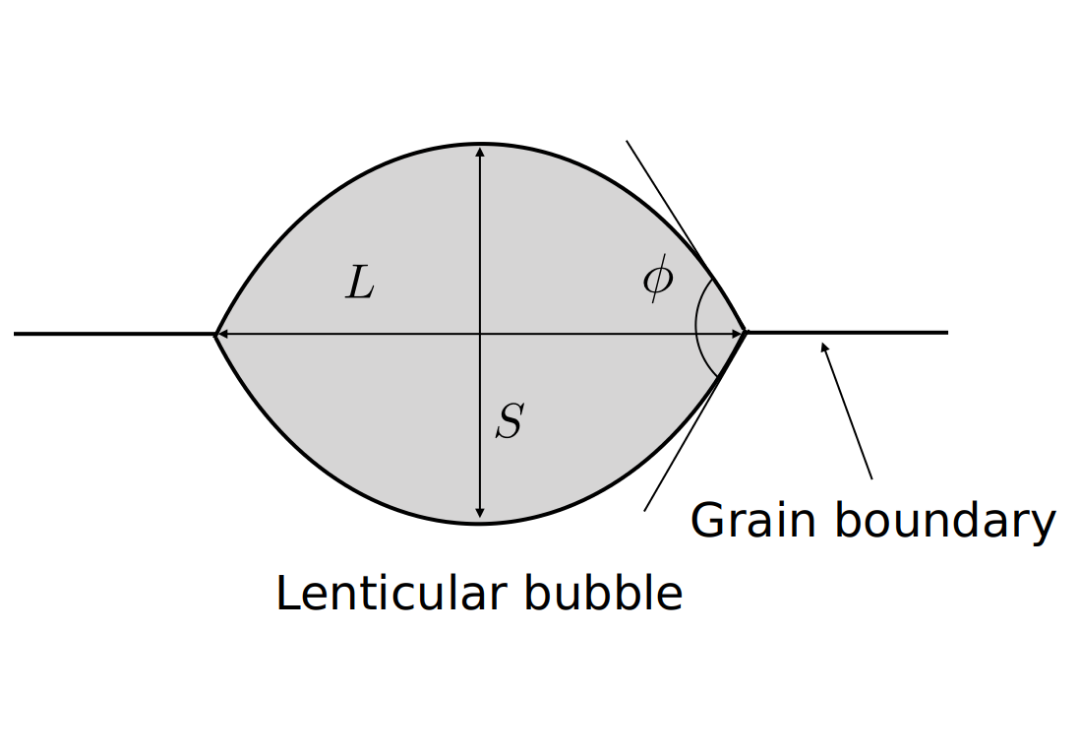
\includegraphics[width=\textwidth]{Chapter3/figures/bub}
        \caption{}
        \label{bubble_geo}
      \end{subfigure} \\
      \begin{subfigure}{0.4\textwidth}
        \centering
        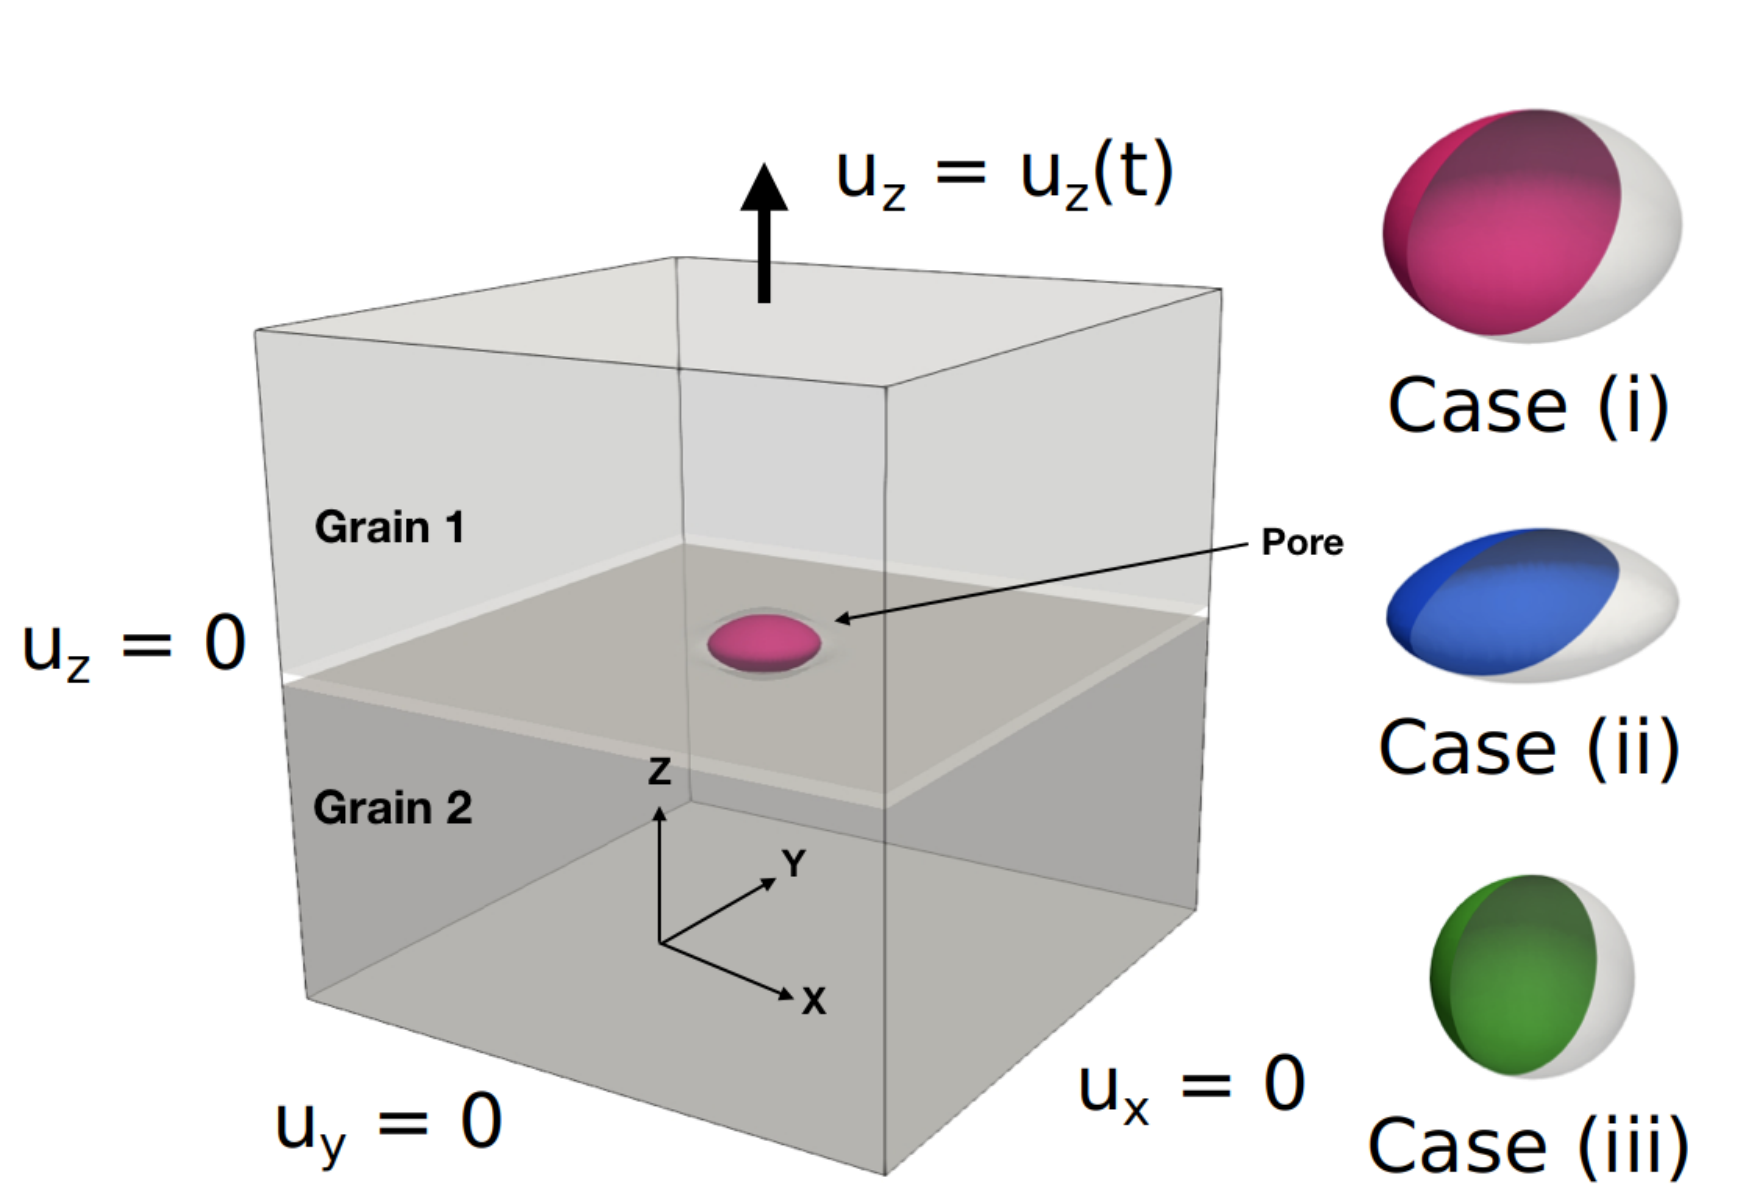
\includegraphics[width=\textwidth]{Chapter3/figures/single_ini}
        \caption{}
        \label{single_ini}
      \end{subfigure}
    \end{tabular}
     &                         
    \begin{subfigure}{0.4\textwidth}
      \centering
      \begin{tikzpicture}
        \begin{axis}[
            width=\textwidth,
            height=1.8\textwidth,
            xlabel=Strain,ylabel=Stress (MPa),
            xmin=0,
            xmax=0.006,
            ymin=0,
            ymax=1000,
            legend style={
                at={(0.02,0.98)},
                anchor=north west,
                nodes={scale=0.8, transform shape},
                text width=1.7in,
                minimum height=0.5in,
                draw=none,
                fill=none
              },
            legend cell align={left},
            every axis plot/.append style={line width=1pt}
          ]
          \addplot +[mark=none,color=black,solid] table[x expr=\thisrowno{2}/40,y=ave_stress_top] {Chapter3/data/single_case1.csv};
          \addplot +[mark=none,color=black,dashed] table[x expr=\thisrowno{2}/40,y=ave_stress_top] {Chapter3/data/single_case2.csv};
          \addplot +[mark=none,color=black,dotted] table[x expr=\thisrowno{2}/40,y=ave_stress_top] {Chapter3/data/single_case3.csv};
          \legend{case (i): Lenticular (large dihedral angle)),case (ii): Lenticular (small dihedral angle)),case (iii): Spherical}
        \end{axis}
      \end{tikzpicture}
      \caption{}
      \label{fig_bubble_geo_stress}
    \end{subfigure} \\
  \end{tabular}
  \caption{ (a) The lenticular geometry is described by the length $L$, the thickness $S$ and the dihedral angle $\phi$. (b) Gas bubble geometry and boundary conditions. (c) Comparison of stress-strain curves for different gas bubble geometries.}
  \label{single_bub}
\end{figure}

%%%%%%%%%%%%%%%%%%%%%%%%%%%%%%%%%%%%%%%%%%%%%%%%%%%%%%%%%%%%%%%%%%%%%%%%%%%%%%%%%%%%%%%%%%%
%%%%%%%%%%%%%%%%%%%%%%%%%%%%%%%%%%%%%%%%%%%%%%%%%%%%%%%%%%%%%%%%%%%%%%%%%%%%%%%%%%%%%%%%%%%
%%%%%%%%%%%%%%%%%%%%%%%%%%%%%%%%%%%%%%%%%%%%%%%%%%%%%%%%%%%%%%%%%%%%%%%%%%%%%%%%%%%%%%%%%%%
%%%%%%%%%%%%%%%%%%%%%%%%%%%%%%%%%%%%%%%%%%%%%%%%%%%%%%%%%%%%%%%%%%%%%%%%%%%%%%%%%%%%%%%%%%%
%%%%%%%%%%%%%%%%%%%%%%%%%%%%%%%%%%%%%%%%%%%%%%%%%%%%%%%%%%%%%%%%%%%%%%%%%%%%%%%%%%%%%%%%%%%
%%%%%%%%%%%%%%%%%%%%%%%%%%%%%%%%%%%%%%%%%%%%%%%%%%%%%%%%%%%%%%%%%%%%%%%%%%%%%%%%%%%%%%%%%%%
%%%%%%%%%%%%%%%%%%%%%%%%%%%%%%%%%%%%%%%%%%%%%%%%%%%%%%%%%%%%%%%%%%%%%%%%%%%%%%%%%%%%%%%%%%%
%%%%%%%%%%%%%%%%%%%%%%%%%%%%%%%%%%%%%%%%%%%%%%%%%%%%%%%%%%%%%%%%%%%%%%%%%%%%%%%%%%%%%%%%%%%
%%%%%%%%%%%%%%%%%%%%%%%%%%%%%%%%%%%%%%%%%%%%%%%%%%%%%%%%%%%%%%%%%%%%%%%%%%%%%%%%%%%%%%%%%%%
%%%%%%%%%%%%%%%%%%%%%%%%%%%%%%%%%%%%%%%%%%%%%%%%%%%%%%%%%%%%%%%%%%%%%%%%%%%%%%%%%%%%%%%%%%%
\subsubsection{Effect of loading}

Next, we study the effect of different loading conditions. Uniaxial, biaxial and triaxial loading conditions are considered. The final crack configurations are shown in \Cref{final_loading}. A change in crack path due to a different loading condition is evident from the figure. For uniaxial loading, cracks propagate along the grain boundaries that are mainly perpendicular to the loading direction. For biaxial loading, crack branching occurs because biaxial loading results in in two positive principal components of the strain tensor of the same order of magnitude. For triaxial loading, cracks propagate along all three directions.
\begin{figure}[!htb]
  \centering
  \begin{subfigure}{0.32\textwidth}
    \centering
    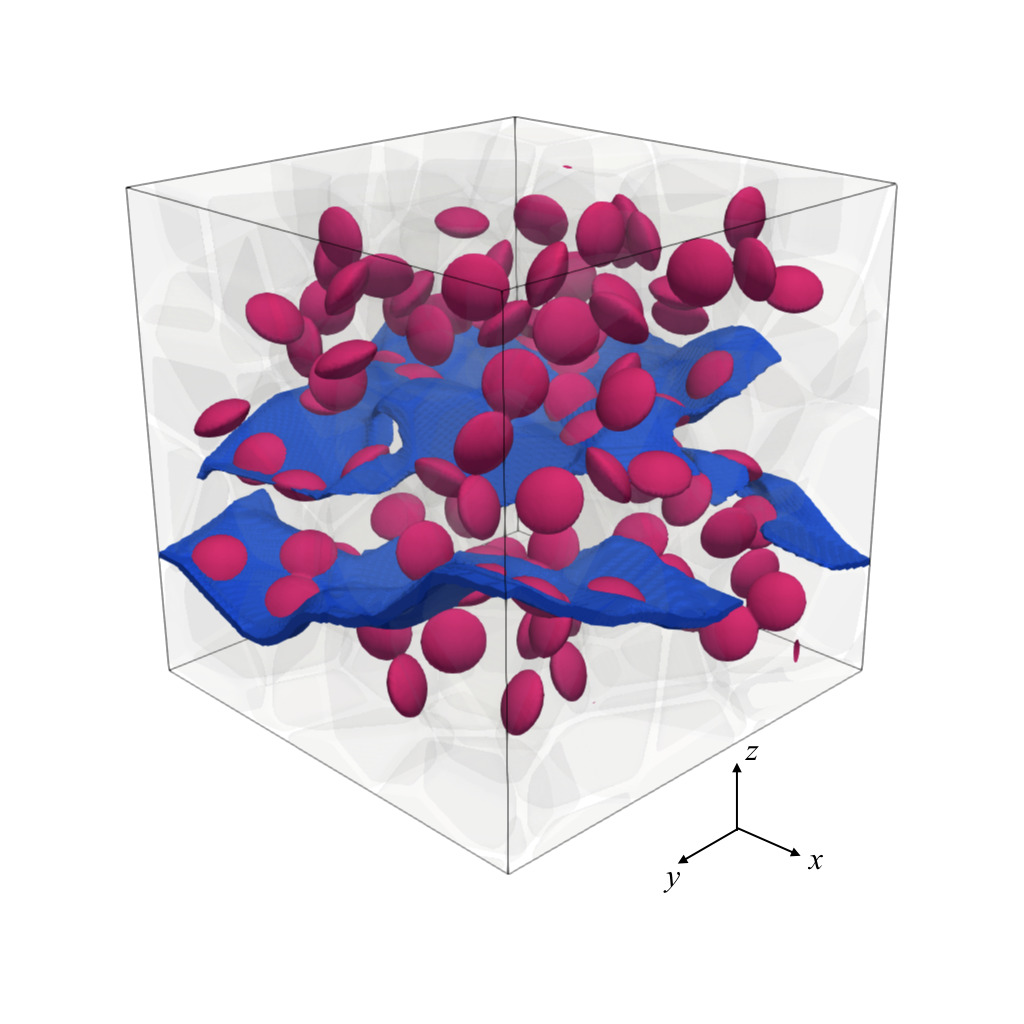
\includegraphics[width=\textwidth]{Chapter3/figures/b100_end}
    \caption{}
    \label{b100_load1}
  \end{subfigure}
  \begin{subfigure}{0.32\textwidth}
    \centering
    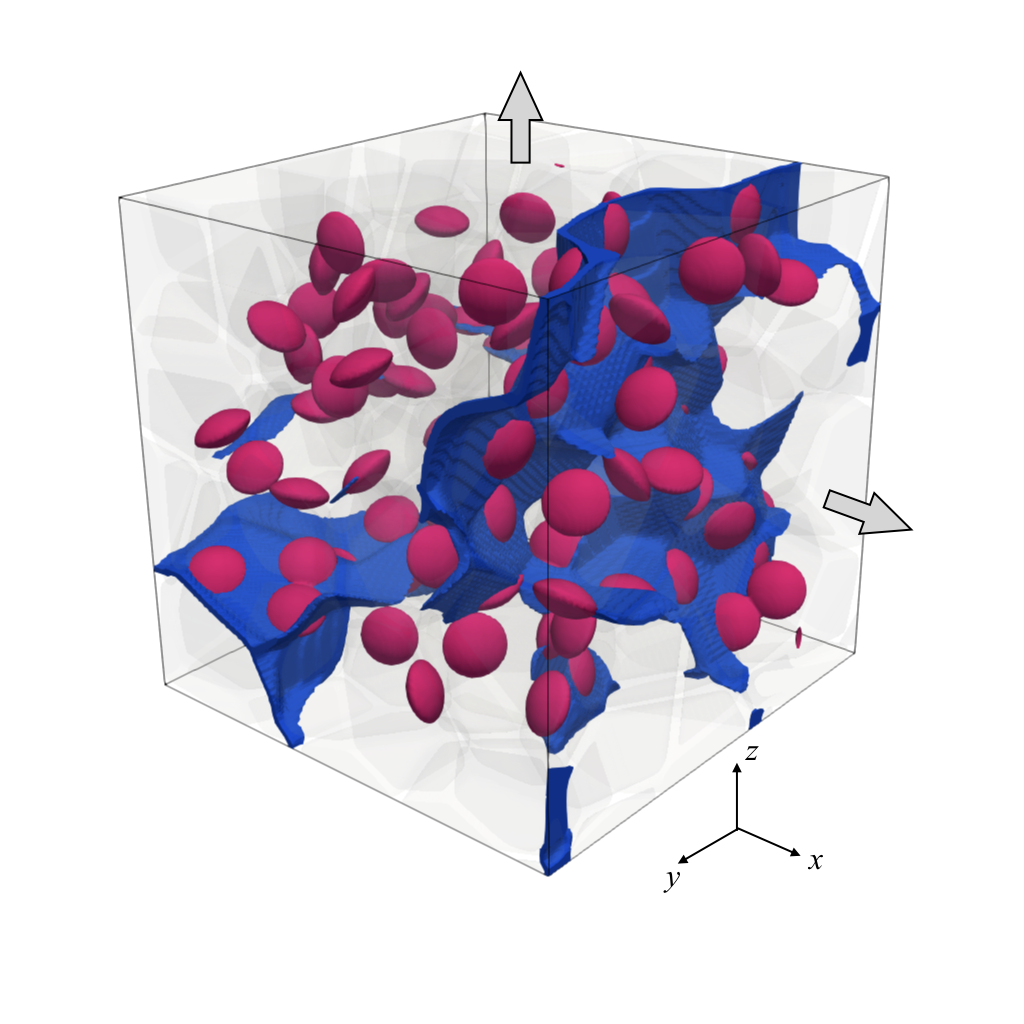
\includegraphics[width=\textwidth]{Chapter3/figures/b100_end_yz}
    \caption{}
    \label{b100_load2}
  \end{subfigure}
  \begin{subfigure}{0.32\textwidth}
    \centering
    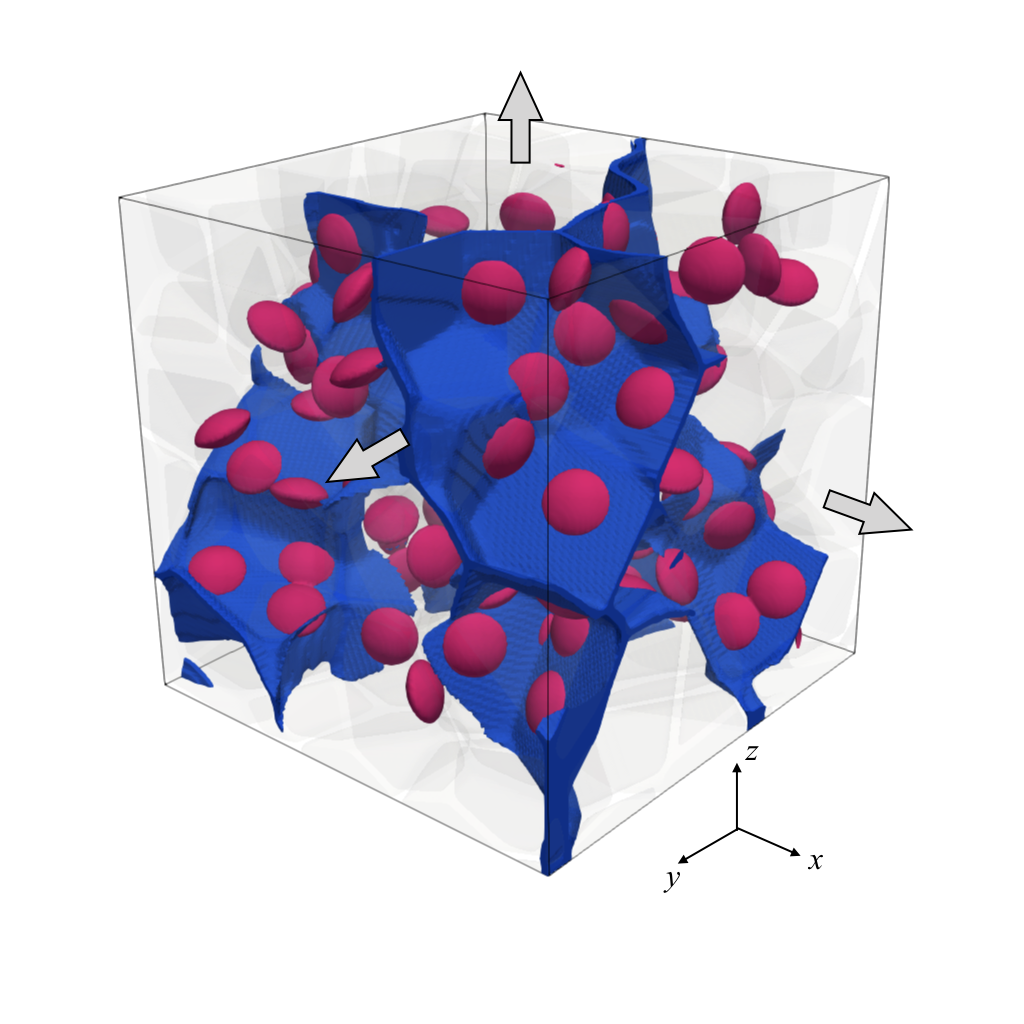
\includegraphics[width=\textwidth]{Chapter3/figures/b100_end_xyz}
    \caption{}
    \label{b100_load3}
  \end{subfigure}
  \caption{ Final configuration (crack surfaces highlighted in blue) for different loading (a) uniaxial (b) biaxial (c) triaxial.}
  \label{final_loading}
\end{figure}

The stress-strain curves are shown in \Cref{fig_loading}. The difference in the slopes during loading is due to the Poisson's effect. The sample under the biaxial and triaxial loading conditions manifest a lower critical fracture strength compared to that under the uniaxial loading condition. The critical strain corresponding to the critical fracture strength under triaxial loading is about half of that under uniaxial loading.

\begin{figure}[!htb]
  \centering
  \begin{tikzpicture}
    \begin{axis}[
        width=0.8\textwidth,
        height=0.4\textwidth,
        xlabel=Strain,ylabel=Stress (MPa),
        xmin=0,
        xmax=0.0025,
        ymin=0,
        ymax=700,
        legend style={at={(0.05,0.95)},anchor=north west},
        legend style={nodes={scale=0.8, transform shape}},
        legend cell align={left},
        every axis plot/.append style={line width=1pt}
      ]
      \addplot +[mark=none,color=black,solid] table[x expr=\thisrowno{2}/40,y=ave_stress_top] {Chapter3/data/b100_y.csv};
      \addplot +[mark=none,color=black,dashed] table[x expr=\thisrowno{5}/40,y=ave_stress_top] {Chapter3/data/b100_yz.csv};
      \addplot +[mark=none,color=black,dotted] table[x expr=\thisrowno{5}/40,y=ave_stress_top] {Chapter3/data/b100_xyz.csv};
      \legend{Uniaxial loading,Biaxial loading,Triaxial loading}
    \end{axis}
  \end{tikzpicture}
  \caption{Comparison of stress-strain curves for different loading conditions.}
  \label{fig_loading}
\end{figure}

%%%%%%%%%%%%%%%%%%%%%%%%%%%%%%%%%%%%%%%%%%%%%%%%%%%%%%%%%%%%%%%%%%%%%%%%%%%%%%%%%%%%%%%%%%%
%%%%%%%%%%%%%%%%%%%%%%%%%%%%%%%%%%%%%%%%%%%%%%%%%%%%%%%%%%%%%%%%%%%%%%%%%%%%%%%%%%%%%%%%%%%
%%%%%%%%%%%%%%%%%%%%%%%%%%%%%%%%%%%%%%%%%%%%%%%%%%%%%%%%%%%%%%%%%%%%%%%%%%%%%%%%%%%%%%%%%%%
%%%%%%%%%%%%%%%%%%%%%%%%%%%%%%%%%%%%%%%%%%%%%%%%%%%%%%%%%%%%%%%%%%%%%%%%%%%%%%%%%%%%%%%%%%%
%%%%%%%%%%%%%%%%%%%%%%%%%%%%%%%%%%%%%%%%%%%%%%%%%%%%%%%%%%%%%%%%%%%%%%%%%%%%%%%%%%%%%%%%%%%
%%%%%%%%%%%%%%%%%%%%%%%%%%%%%%%%%%%%%%%%%%%%%%%%%%%%%%%%%%%%%%%%%%%%%%%%%%%%%%%%%%%%%%%%%%%
%%%%%%%%%%%%%%%%%%%%%%%%%%%%%%%%%%%%%%%%%%%%%%%%%%%%%%%%%%%%%%%%%%%%%%%%%%%%%%%%%%%%%%%%%%%
%%%%%%%%%%%%%%%%%%%%%%%%%%%%%%%%%%%%%%%%%%%%%%%%%%%%%%%%%%%%%%%%%%%%%%%%%%%%%%%%%%%%%%%%%%%
%%%%%%%%%%%%%%%%%%%%%%%%%%%%%%%%%%%%%%%%%%%%%%%%%%%%%%%%%%%%%%%%%%%%%%%%%%%%%%%%%%%%%%%%%%%
%%%%%%%%%%%%%%%%%%%%%%%%%%%%%%%%%%%%%%%%%%%%%%%%%%%%%%%%%%%%%%%%%%%%%%%%%%%%%%%%%%%%%%%%%%%
\subsubsection{Effect of porosity}

In 2D, under plane-strain assumptions, the porosity represented by a planar bubble is computed by extruding it along the out-of-plane direction, which overestimates the actual porosity. In order to obtain a reasonable correlation between the critical fracture strength and the porosity, a 3D model is necessary.

To study the effect of porosity, consider an REV with side length \SI{40}{\micro\meter}. Grain centroids are generated from a random close-packing (RCP) voronoi structure. The RCP structures can be realized by a spatial sampling process known as Maximal Poisson-disk Sampling (MPS) \cite{Ebeida2012}. For the RCP voronoi structure, the average aspect ratio of each voronoi cell is approximately 1 and an equiaxed grain structure is provided.

The influence of the voronoi structure on fracture properties can be isolated by considering a specific realization of RCP. The realization under consideration consists of 77 grains and the average radius of grains is \SI{9.4}{\micro\meter}. As shown in \Cref{ini_final_porosity}, 50, 100 and 150 gas bubbles are randomly distributed over the grain boundaries, with corresponding porosity values $2.02\%$, $4.04\%$ and $6.06\%$, respectively. All gas bubbles have a lenticular shape with $L = \SI{6.4}{\micro\meter}$, $S = \SI{4}{\micro\meter}$, and $\phi=\SI{128}{\degree}$. Symmetric boundary conditions are prescribed and a uniform displacement is applied on the top of the REV.

Final configurations of the approximated crack surfaces are shown in \Cref{ini_final_porosity}, where, in general, cracks propagate perpendicular to the direction of the applied load.
\begin{figure}[!htb]
  \centering
  \begin{subfigure}{0.32\textwidth}
    \centering
    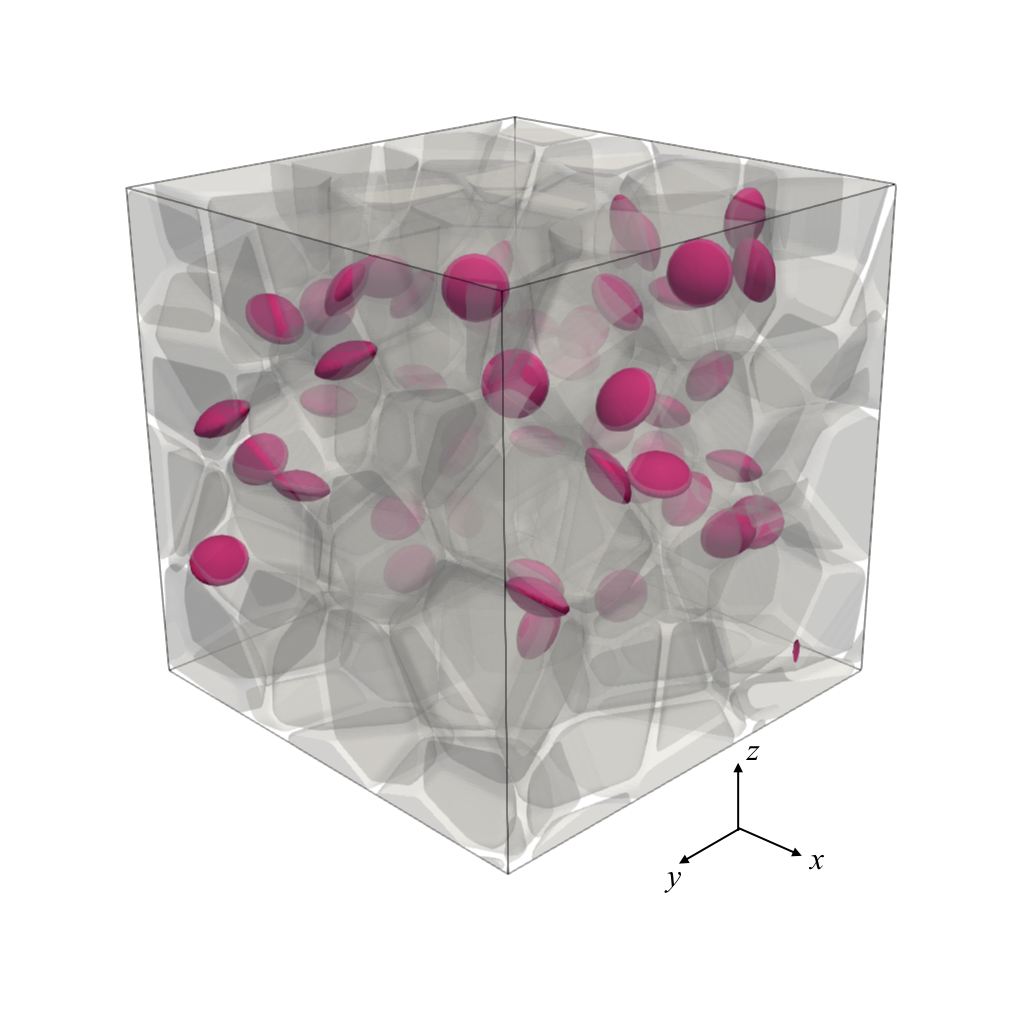
\includegraphics[width=\textwidth]{Chapter3/figures/b50_ini_new}
    \caption{}
    \label{b50_ini}
  \end{subfigure}
  \begin{subfigure}{0.32\textwidth}
    \centering
    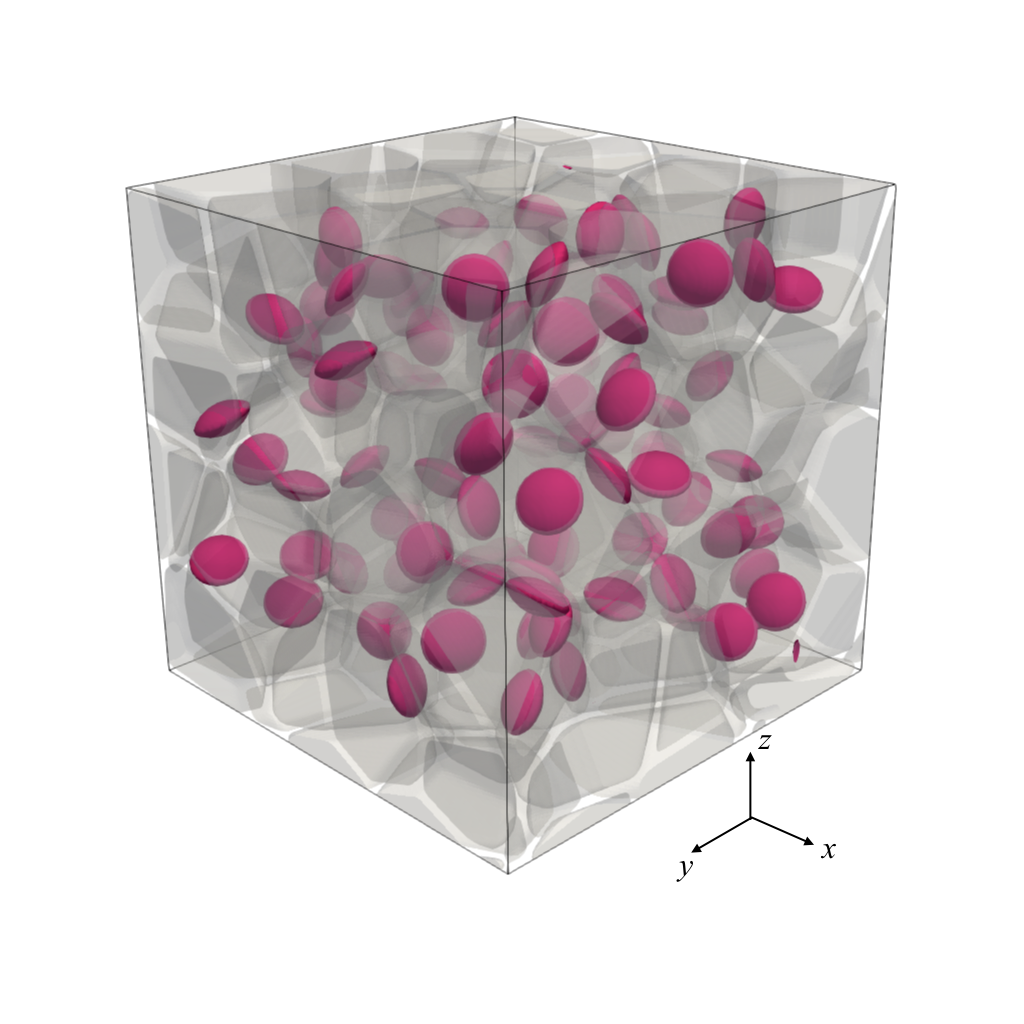
\includegraphics[width=\textwidth]{Chapter3/figures/b100_ini_new}
    \caption{}
    \label{b100_ini}
  \end{subfigure}
  \begin{subfigure}{0.32\textwidth}
    \centering
    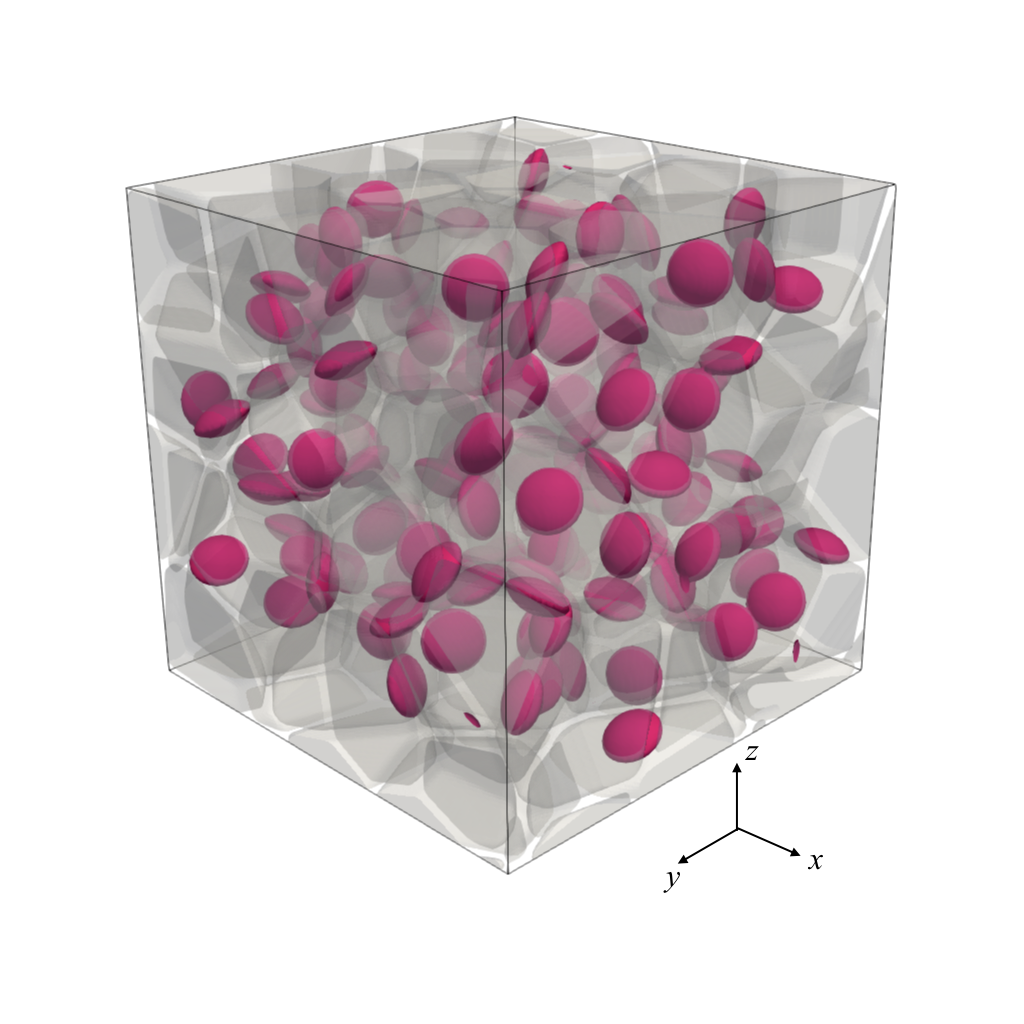
\includegraphics[width=\textwidth]{Chapter3/figures/b150_ini_new}
    \caption{}
    \label{b150_ini}
  \end{subfigure}
  \begin{subfigure}{0.32\textwidth}
    \centering
    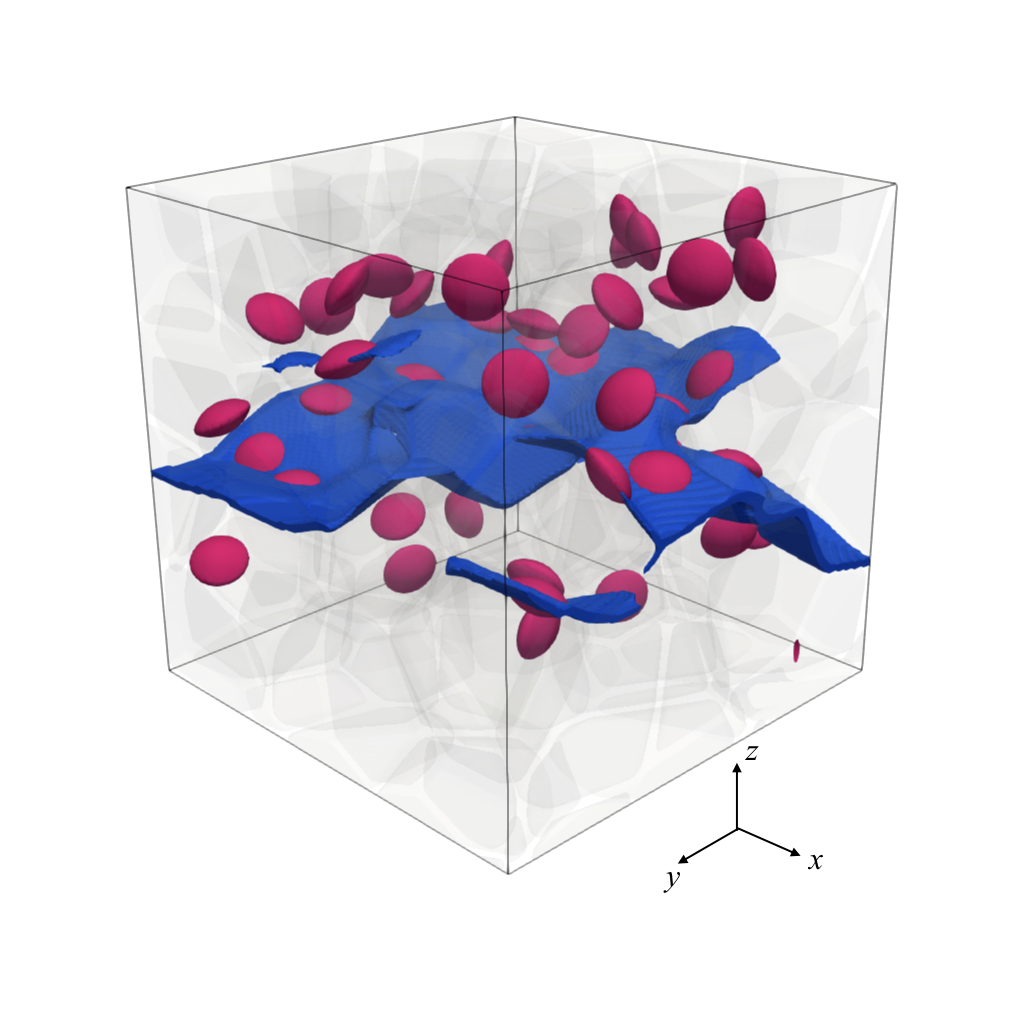
\includegraphics[width=\textwidth]{Chapter3/figures/b50_end}
    \caption{}
    \label{b50_end}
  \end{subfigure}
  \begin{subfigure}{0.32\textwidth}
    \centering
    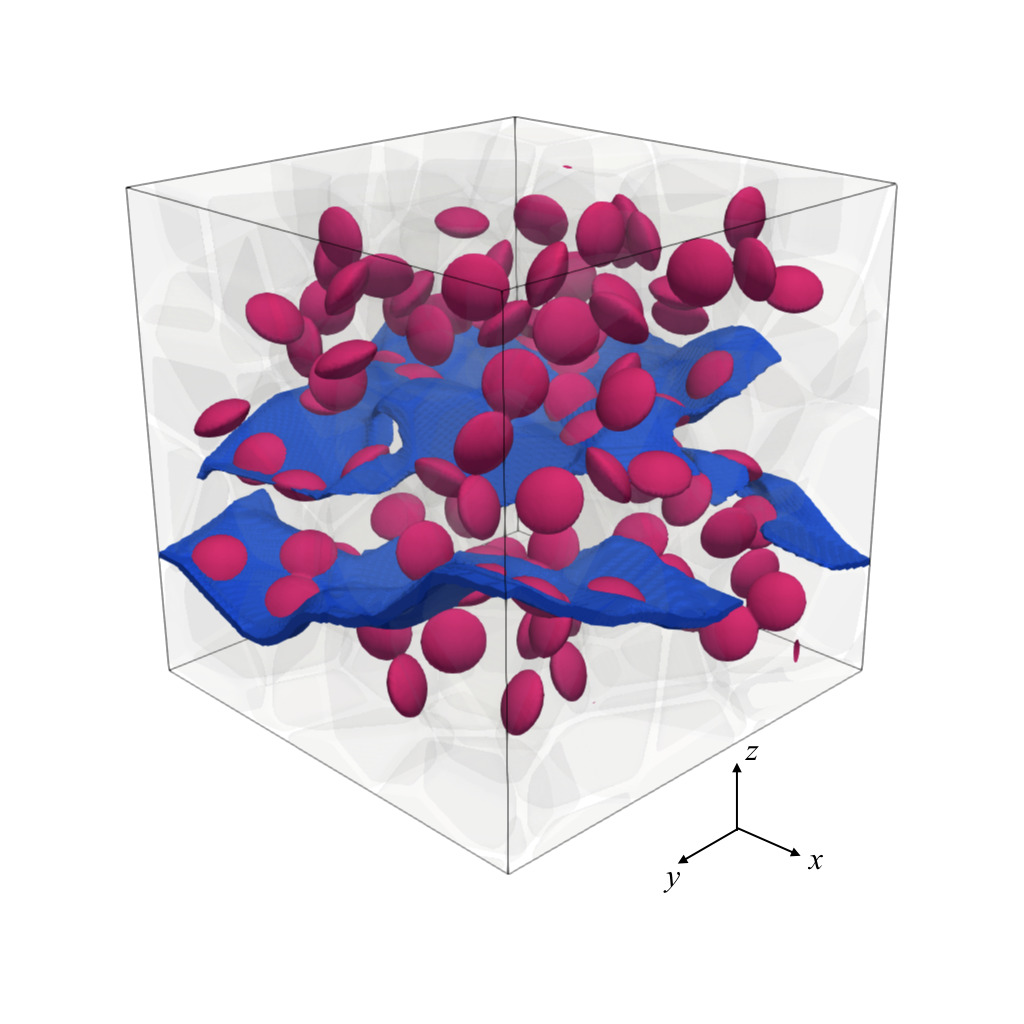
\includegraphics[width=\textwidth]{Chapter3/figures/b100_end}
    \caption{}
    \label{b100_end}
  \end{subfigure}
  \begin{subfigure}{0.32\textwidth}
    \centering
    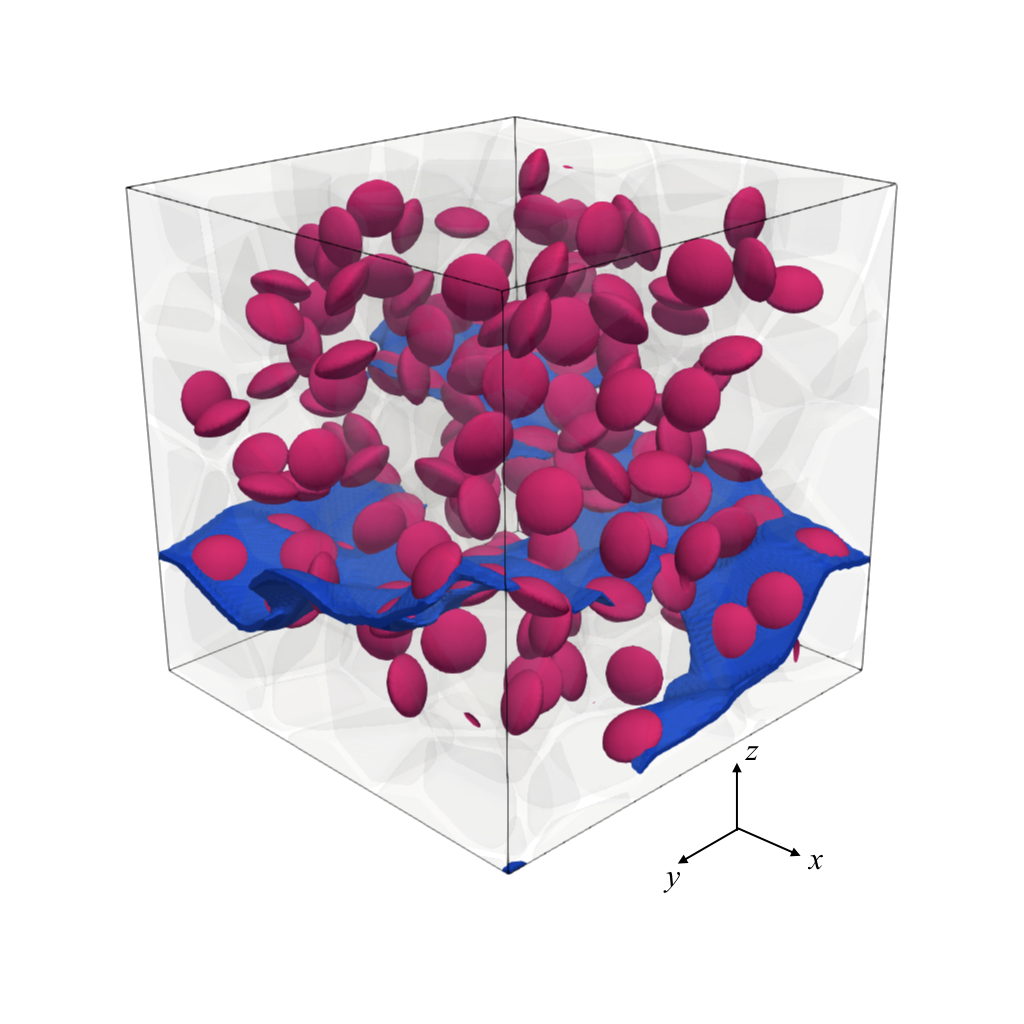
\includegraphics[width=\textwidth]{Chapter3/figures/b150_end}
    \caption{}
    \label{b150_end}
  \end{subfigure}
  \caption{ (a-c) Initial configuration of REVs with an average grain size of \SI{9.4}{\micro\meter}. (d-f) Final configuration (crack surfaces highlighted in blue) for REVs. Different porosity values are considered: (a, d) $2.02\%$, (b, e) $4.04\%$, (c, f) $6.06\%$. }
  \label{ini_final_porosity}
\end{figure}

\begin{figure}[!htb]
  \centering
  \begin{tikzpicture}
    \begin{axis}[
        width=0.8\textwidth,
        height=0.4\textwidth,
        xlabel=Strain,ylabel=Stress (MPa),
        xmin=0,
        xmax=0.0025,
        ymin=0,
        ymax=700,
        legend style={
            at={(0.02,0.98)},
            anchor=north west,
            nodes={scale=0.8, transform shape},
            draw=none,
            fill=none
          },
        legend cell align={left},
        every axis plot/.append style={line width=1pt}
      ]
      \addplot +[mark=none,color=black,solid] table[x expr=\thisrowno{2}/40,y=ave_stress_top] {Chapter3/data/b50_out.csv};
      \addplot +[mark=none,color=black,dashed] table[x expr=\thisrowno{2}/40,y=ave_stress_top] {Chapter3/data/b100_out.csv};
      \addplot +[mark=none,color=black,dotted] table[x expr=\thisrowno{2}/40,y=ave_stress_top] {Chapter3/data/b150_out.csv};
      \legend{Porosity 2.02\% (50 bubbles),Porosity 4.04\% (100 bubbles),Porosity 6.06\% (150 bubbles)}
    \end{axis}
  \end{tikzpicture}
  \caption{Comparison of stress-strain curves for different porosity values.}
  \label{fig_porosity}
\end{figure}

It is worth noting that cracks keep propagating after initiation without any increase in the applied stress, which suggests that a snap-back is likely to take place after crack initiation and a mixed force-displacement control is necessary to follow the actual stress-strain curve without loss of information. However, we argue that the a simple displacement control suffices to obtain the critical fracture strength -- the maximum stress value along the stress-strain curve. From \Cref{fig_porosity}, we conclude that an increase in porosity leads to a higher probability of crack initiation at lower stress state and consequently a decrease in the critical fracture strength.

To describe the porosity, average gas bubble and grain size effect on fracture strength, an exponential functional form obtained from biaxial flexure test has been reported in \cite{oguma_1982}:
\begin{align}
  \dfrac{\sigma_c}{\sigma_0} = \exp(-a \times \text{porosity})
\end{align}
The critical fracture strength is normalized with respect to $\sigma_0$. To benchmark with experiments, $\sigma_0$ is obtained by substituting the average grain and bubble size of \SI{9.4}{\micro\meter} and \SI{5.2}{\micro\meter}. To give proper error bounds on our numerical predictions, five trial calculations were performed on five different realizations of the spatial distribution of bubbles for each porosity level. The fracture strength values obtained from 15 realizations of 3 porosity levels are summarized in \Cref{fs15}. The fitted $\sigma_0$ is \SI{198}{\mega\pascal}, \SI{693}{\mega\pascal} and \SI{697.8}{\mega\pascal} and the coefficient $a$ is 0.057, 0.14 and 0.04, for experiment, 2D simulations and 3D simulations, respectively.
A comparison of the experimental model, previous 2D simulations \cite{pritam_2016} and current 3D simulations is shown in \Cref{fig_rfit_porosity}. In particular, the $95\%$ confidence interval for the 3D simulations is shown in stripes. It shows that the 3D simulation has significant improvement towards the prediction of the dependence of the critical fracture strength on porosity. It is worth mentioning that the difference between simulation predictions of $\sigma_0$ and experimental values could be due to the fact that the transgranular fracture observed in experiments \cite{evans_1969} has not been incorporated into the current numerical model.

\begin{table}[!htb]
  \centering
  \caption{Summary of fracture strength obtained from 15 realizations of 3 porosity values. R denotes the realization index.}
  \begin{tabular}{*6c}
    \toprule
    Porosity (\%) & \multicolumn{5}{c}{Critical fracture strength (\SI{}{\mega\pascal})}                                 \\
    \midrule
                  & R1                                                                   & R2    & R3    & R4    & R5    \\
    \midrule
    2.02          & 631.4                                                                & 657.4 & 645.6 & 663.4 & 630.7 \\
    4.04          & 609.8                                                                & 555.6 & 605.5 & 611.2 & 589.2 \\
    6.06          & 540.0                                                                & 530.8 & 557.0 & 563.2 & 567.9 \\
    \bottomrule
  \end{tabular}
  \label{fs15}
\end{table}

\begin{figure}[!htb]
  \centering
  \begin{tikzpicture}
    \begin{axis}[
        width=0.8\textwidth,
        height=0.4\textwidth,
        xlabel=Porosity (\%),ylabel=Normalized fracture strength,
        xmin=0,
        xmax=10,
        ymin=0,
        ymax=1.2,
        legend style={at={(0.05,0.05)},anchor=south west},
        legend style={nodes={scale=0.8, transform shape}},
        legend cell align={left},
        every axis plot/.append style={line width=1pt}
      ]
      % plot the confidence interval band
      \addplot [name path=upper,draw=none,domain=0:10,forget plot] {727/697.8*exp(-0.02925*x)};
      \addplot [name path=lower,draw=none,domain=0:10,forget plot] {668.5/697.8*exp(-0.04959*x)};
      \tikzfillbetween[of=upper and lower]{pattern=north west lines};
      % experiment
      \addplot +[mark=none,color=black,solid,domain=0:10] {exp(-0.057*x)};
      % 3D
      \addplot +[mark=none,color=black,dashed,domain=0:10] {exp(-0.03942*x)};
      % 2D
      \addplot +[mark=none,color=black,dotted,domain=0:10] {exp(-0.14*x)};
      \legend{Experiment (Oguma et. al.),3D simulation (fitted curve), 2D simulation (fitted curve)}
    \end{axis}
  \end{tikzpicture}
  \caption{Variation in normalized fracture strength with changing porosity. In the current chapter, five trial calculations were performed for each porosity level, and each calculation was based on one realization of the spatial distribution of bubbles. The 95\% confidence interval is shown in stripes.}
  \label{fig_rfit_porosity}
\end{figure}

%%%%%%%%%%%%%%%%%%%%%%%%%%%%%%%%%%%%%%%%%%%%%%%%%%%%%%%%%%%%%%%%%%%%%%%%%%%%%%%%%%%%%%%%%%%
%%%%%%%%%%%%%%%%%%%%%%%%%%%%%%%%%%%%%%%%%%%%%%%%%%%%%%%%%%%%%%%%%%%%%%%%%%%%%%%%%%%%%%%%%%%
%%%%%%%%%%%%%%%%%%%%%%%%%%%%%%%%%%%%%%%%%%%%%%%%%%%%%%%%%%%%%%%%%%%%%%%%%%%%%%%%%%%%%%%%%%%
%%%%%%%%%%%%%%%%%%%%%%%%%%%%%%%%%%%%%%%%%%%%%%%%%%%%%%%%%%%%%%%%%%%%%%%%%%%%%%%%%%%%%%%%%%%
%%%%%%%%%%%%%%%%%%%%%%%%%%%%%%%%%%%%%%%%%%%%%%%%%%%%%%%%%%%%%%%%%%%%%%%%%%%%%%%%%%%%%%%%%%%
%%%%%%%%%%%%%%%%%%%%%%%%%%%%%%%%%%%%%%%%%%%%%%%%%%%%%%%%%%%%%%%%%%%%%%%%%%%%%%%%%%%%%%%%%%%
%%%%%%%%%%%%%%%%%%%%%%%%%%%%%%%%%%%%%%%%%%%%%%%%%%%%%%%%%%%%%%%%%%%%%%%%%%%%%%%%%%%%%%%%%%%
%%%%%%%%%%%%%%%%%%%%%%%%%%%%%%%%%%%%%%%%%%%%%%%%%%%%%%%%%%%%%%%%%%%%%%%%%%%%%%%%%%%%%%%%%%%
%%%%%%%%%%%%%%%%%%%%%%%%%%%%%%%%%%%%%%%%%%%%%%%%%%%%%%%%%%%%%%%%%%%%%%%%%%%%%%%%%%%%%%%%%%%
%%%%%%%%%%%%%%%%%%%%%%%%%%%%%%%%%%%%%%%%%%%%%%%%%%%%%%%%%%%%%%%%%%%%%%%%%%%%%%%%%%%%%%%%%%%
\subsection{High burnup structure fragmentation}

Next, we adopt the quasi-brittle fracture model to simulate fission-gas-induced intergranular fracture of UO$_2$ HBS. A two-dimensional REV with side length $L = \SI{3}{\micro\meter}$ is considered, and plane-strain conditions are assumed to hold. The material properties and model parameters are summarized in \Cref{table: HBS material properties}. The critical fracture energy of UO$_2$ is taken to be \SI{0.022}{\milli\joule\per\cubic\milli\meter} \cite{oguma_1982}.
Due to the lack of experimental data, the fracture toughness $\Gc^g$ is assumed to be \SI{1.2e-6}{\milli\joule\per\cubic\milli\meter} and the Griffith's characteristic length $l_\text{ch} = \dfrac{\Gc}{2\psi_c} \approx \SI{22.78}{\nano\meter}$. The domain is uniformly discretized with \texttt{QUAD4} elements with element size of $\SI{0.005}{\micro\meter}$.

\begin{table}[!htb]
  \centering
  \caption{Parameters and material properties used in the fission-gas-induced HBS fracture simulations.}
  \label{table: HBS material properties}
  \begin{tabular}{ r c c c c }
    \toprule
    \textbf{Property}                 & \textbf{Symbol} & \textbf{Value} & \textbf{Unit}                             & \textbf{Reference} \\
    \midrule
    Young's modulus                   & $E$             & 385            & \SI{}{\giga\pascal}                       & \cite{govers_2007} \\
    Critical fracture energy          & $\psi_c$        & 0.022          & \SI{}{\milli\joule\per\cubic\milli\meter} & \cite{oguma_1982}   \\
    Grain boundary fracture toughness & $\Gc^g$         & \SI{1.2e-6}{}  & \SI{}{\milli\joule\per\cubic\milli\meter} &                    \\
    Grain fracture toughness          & $\Gc^b$         & \SI{1.2e-5}{}  & \SI{}{\milli\joule\per\cubic\milli\meter} &                    \\
    Phase-field regularization length & $l$             & 0.01           & \SI{}{\micro\meter}                       &                    \\
    \bottomrule
  \end{tabular}
\end{table}

%%%%%%%%%%%%%%%%%%%%%%%%%%%%%%%%%%%%%%%%%%%%%%%%%%%%%%%%%%%%%%%%%%%%%%%%%%%%%%%%%%%%%%%%%%%
%%%%%%%%%%%%%%%%%%%%%%%%%%%%%%%%%%%%%%%%%%%%%%%%%%%%%%%%%%%%%%%%%%%%%%%%%%%%%%%%%%%%%%%%%%%
%%%%%%%%%%%%%%%%%%%%%%%%%%%%%%%%%%%%%%%%%%%%%%%%%%%%%%%%%%%%%%%%%%%%%%%%%%%%%%%%%%%%%%%%%%%
%%%%%%%%%%%%%%%%%%%%%%%%%%%%%%%%%%%%%%%%%%%%%%%%%%%%%%%%%%%%%%%%%%%%%%%%%%%%%%%%%%%%%%%%%%%
%%%%%%%%%%%%%%%%%%%%%%%%%%%%%%%%%%%%%%%%%%%%%%%%%%%%%%%%%%%%%%%%%%%%%%%%%%%%%%%%%%%%%%%%%%%
%%%%%%%%%%%%%%%%%%%%%%%%%%%%%%%%%%%%%%%%%%%%%%%%%%%%%%%%%%%%%%%%%%%%%%%%%%%%%%%%%%%%%%%%%%%
%%%%%%%%%%%%%%%%%%%%%%%%%%%%%%%%%%%%%%%%%%%%%%%%%%%%%%%%%%%%%%%%%%%%%%%%%%%%%%%%%%%%%%%%%%%
%%%%%%%%%%%%%%%%%%%%%%%%%%%%%%%%%%%%%%%%%%%%%%%%%%%%%%%%%%%%%%%%%%%%%%%%%%%%%%%%%%%%%%%%%%%
%%%%%%%%%%%%%%%%%%%%%%%%%%%%%%%%%%%%%%%%%%%%%%%%%%%%%%%%%%%%%%%%%%%%%%%%%%%%%%%%%%%%%%%%%%%
%%%%%%%%%%%%%%%%%%%%%%%%%%%%%%%%%%%%%%%%%%%%%%%%%%%%%%%%%%%%%%%%%%%%%%%%%%%%%%%%%%%%%%%%%%%
\subsubsection{LOCA pressure transients}

We begin by investigating gas-pressure-induced fracture during LOCA-driven temperature transients. During a LOCA transient, temperatures in the fuel rod increase rapidly, leading to increased pressure in the gas contained within the bubbles. The temperature as a function of time at the edge of a representative pellet for each rod is obtained from simulation of the Studsvik Rod 196 experiment \cite{STUDSVIK} using the engineering-scale fuel performance code BISON \cite{WILLIAMSON2020}. The temperature transient is used as an input to the Kim-Kim-Suzuki (KKS) phase-field model \cite{Aagesen2020} to determine the pressure as a function of time. In the KKS model, the gas pressure is assumed to be \SI{100}{\mega\pascal} during steady-state reactor operation at \SI{700}{\kelvin}. The Studsvik experiment is initialized with a fixed temperature $T = \SI{572.6}{\kelvin}$ at the outer surface prior to the transient, resulting in a decrease in the pressure from \SI{100}{\mega\pascal} to below \SI{80}{\mega\pascal}. The pressure is assumed to be known in the quasi-brittle fracture model to simulate crack nucleation and propagation in the surrounding regions of the individual bubbles.

Two bubble radii (\SI{0.25}{\micro\meter} and \SI{0.5}{\micro\meter}) are considered, and no loading is applied on the exterior. The resulting fracture patterns are shown in \Cref{fig:r25}. With the smaller bubble, two cracks propagate from the bubble towards the outer surface. With a larger bubble, only one major crack propagates to the free surface, and other minor cracks are arrested. Cracks nucleate when tensile stress on the bubble-matrix interface reaches the critical fracture strength. The critical pressures are \SI{120.17}{\mega\pascal} and \SI{89.69}{\mega\pascal} for the small and large bubbles, respectively. The critical pressure is significantly lower for the larger bubble.

\begin{figure}[htb!]
  \centering
  \begin{subfigure}[t]{0.32\linewidth}
    \centering
    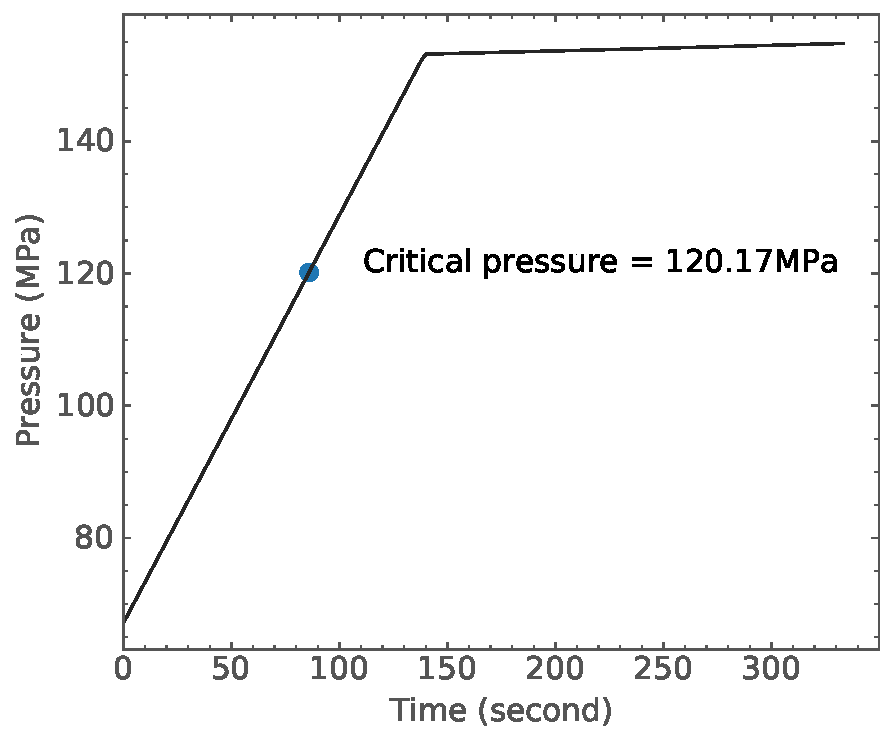
\includegraphics[width=\linewidth]{Chapter3/figures/bubble_pressure_r0.25_ext0_rod196}
    \caption{}
  \end{subfigure}
  \begin{subfigure}[t]{0.32\linewidth}
    \centering
    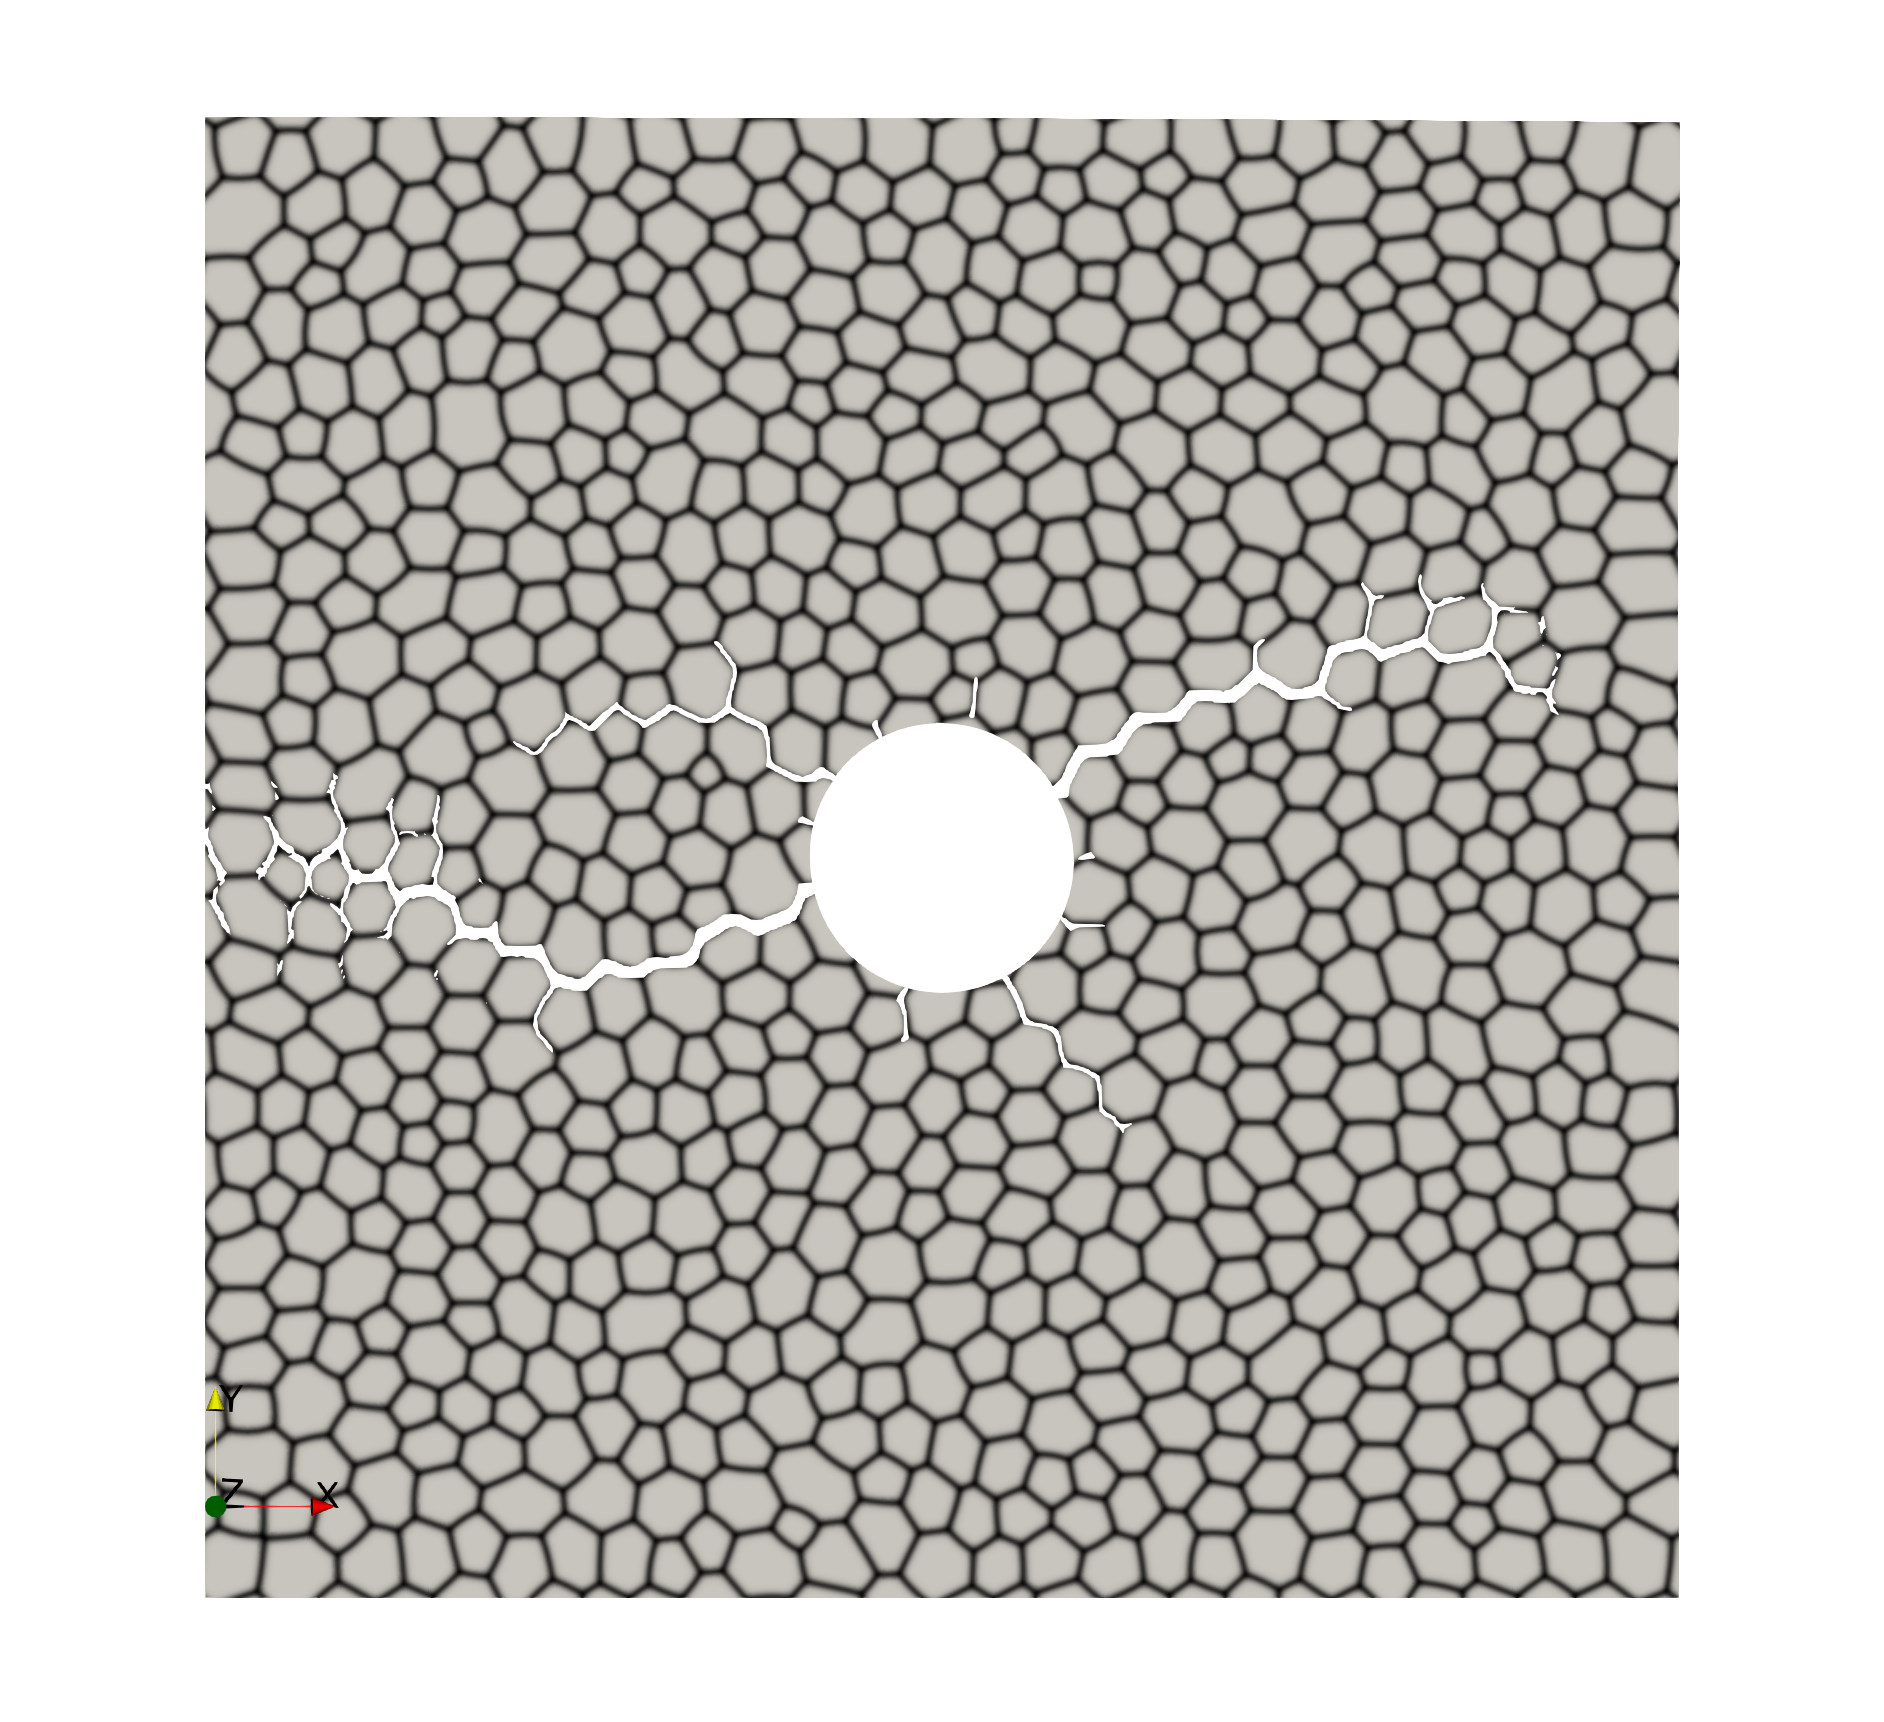
\includegraphics[width=\linewidth]{Chapter3/figures/r25_ext0}
    \caption{}
  \end{subfigure}
  \begin{subfigure}[t]{0.32\linewidth}
    \centering
    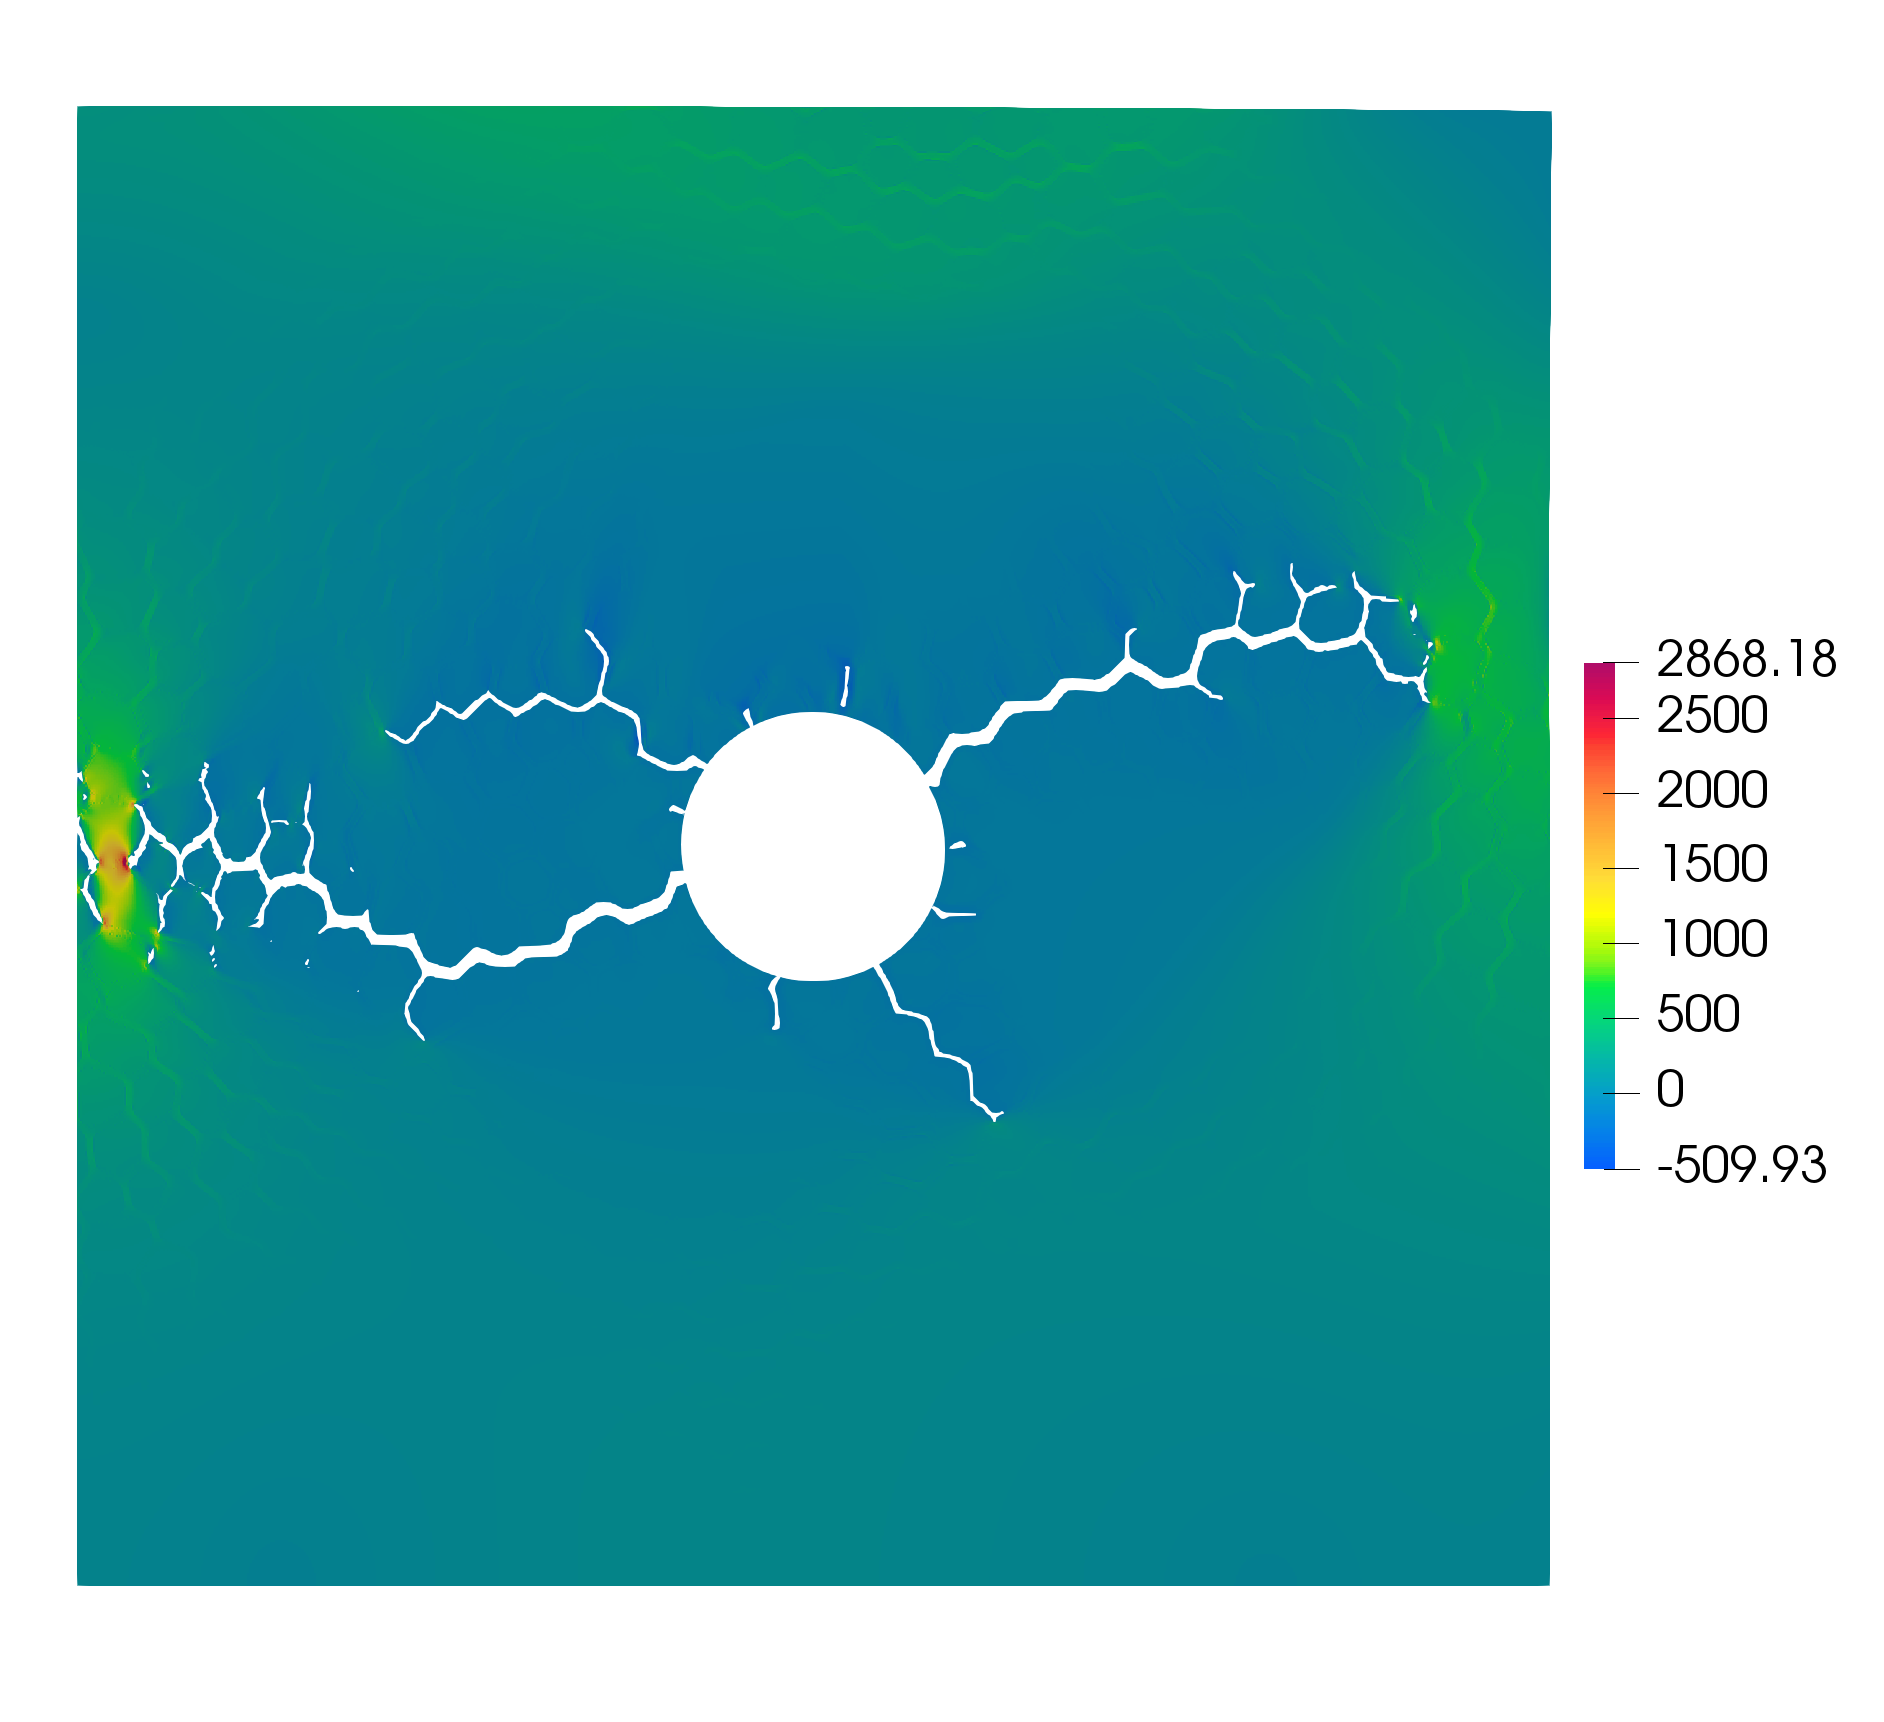
\includegraphics[width=\linewidth]{Chapter3/figures/r25_ext0_stress}
    \caption{}
  \end{subfigure}\\
  \begin{subfigure}[t]{0.32\linewidth}
    \centering
    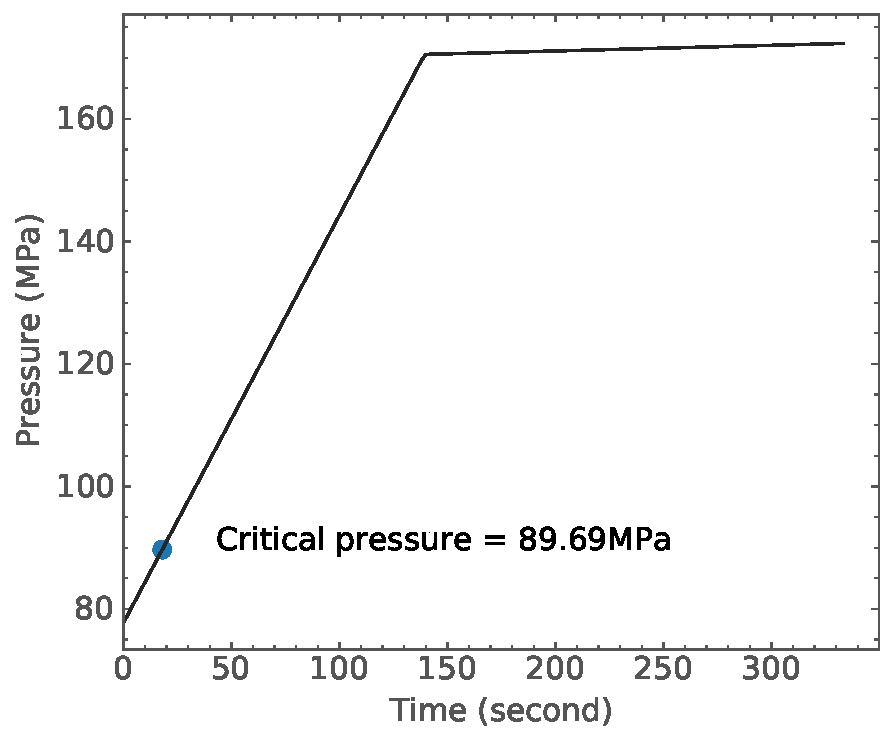
\includegraphics[width=\linewidth]{Chapter3/figures/bubble_pressure_r0.5_ext0_rod196}
    \caption{}
  \end{subfigure}
  \begin{subfigure}[t]{0.32\linewidth}
    \centering
    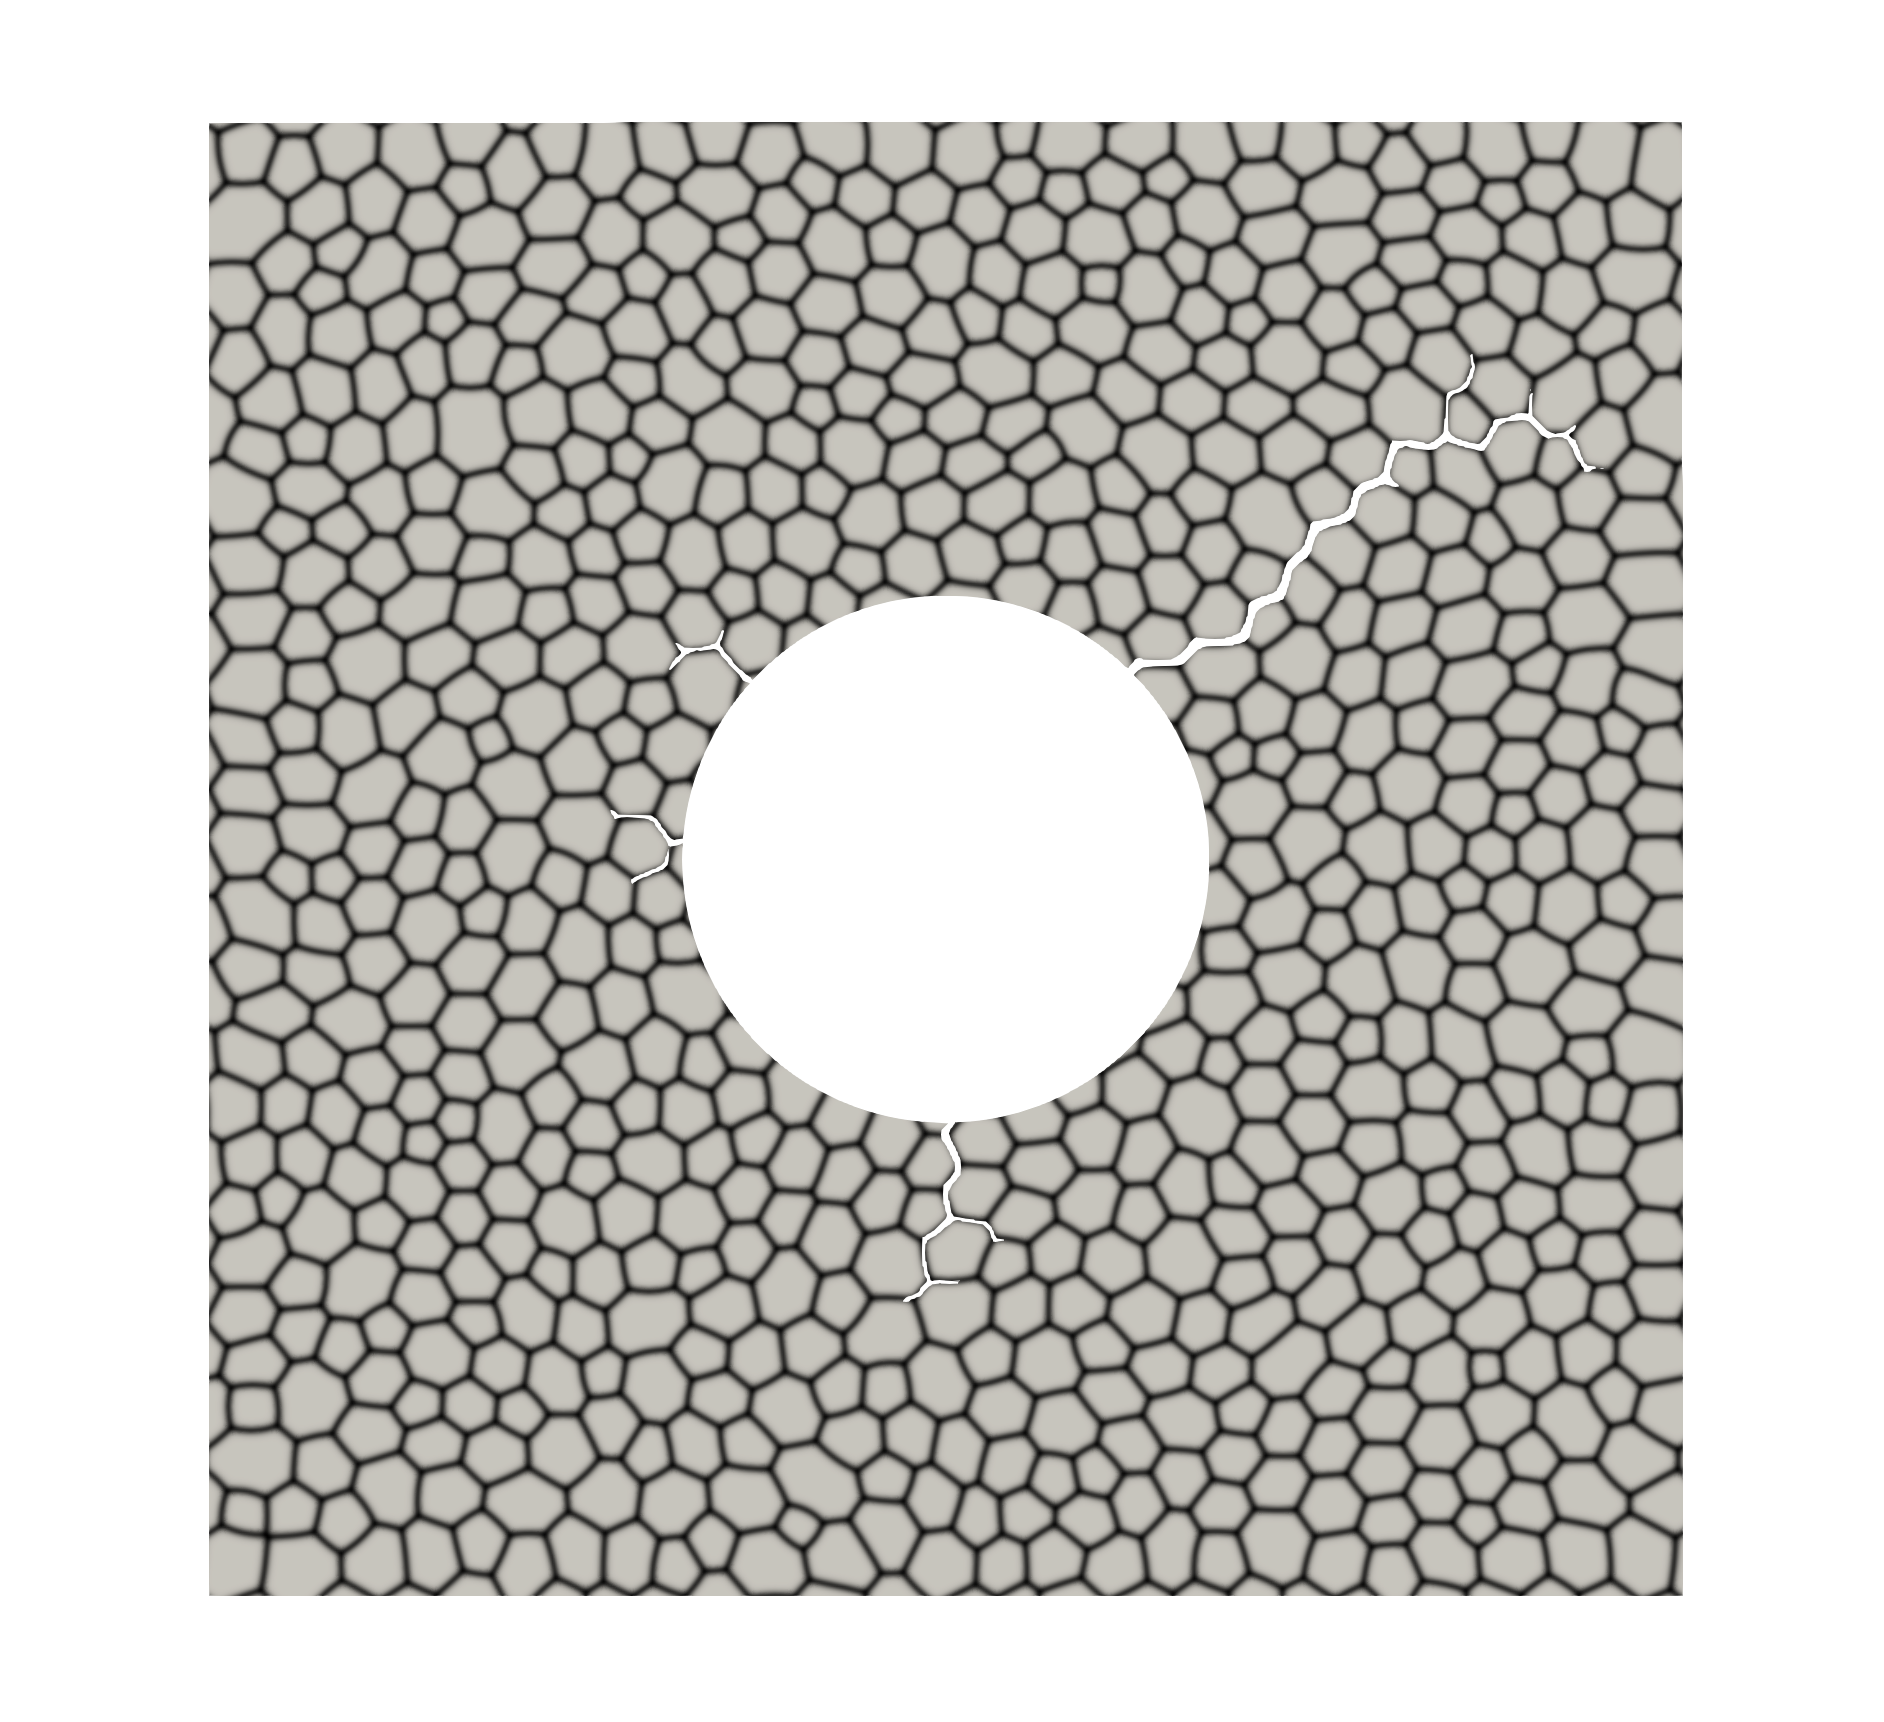
\includegraphics[width=\linewidth]{Chapter3/figures/r5_ext0}
    \caption{}
  \end{subfigure}
  \begin{subfigure}[t]{0.32\linewidth}
    \centering
    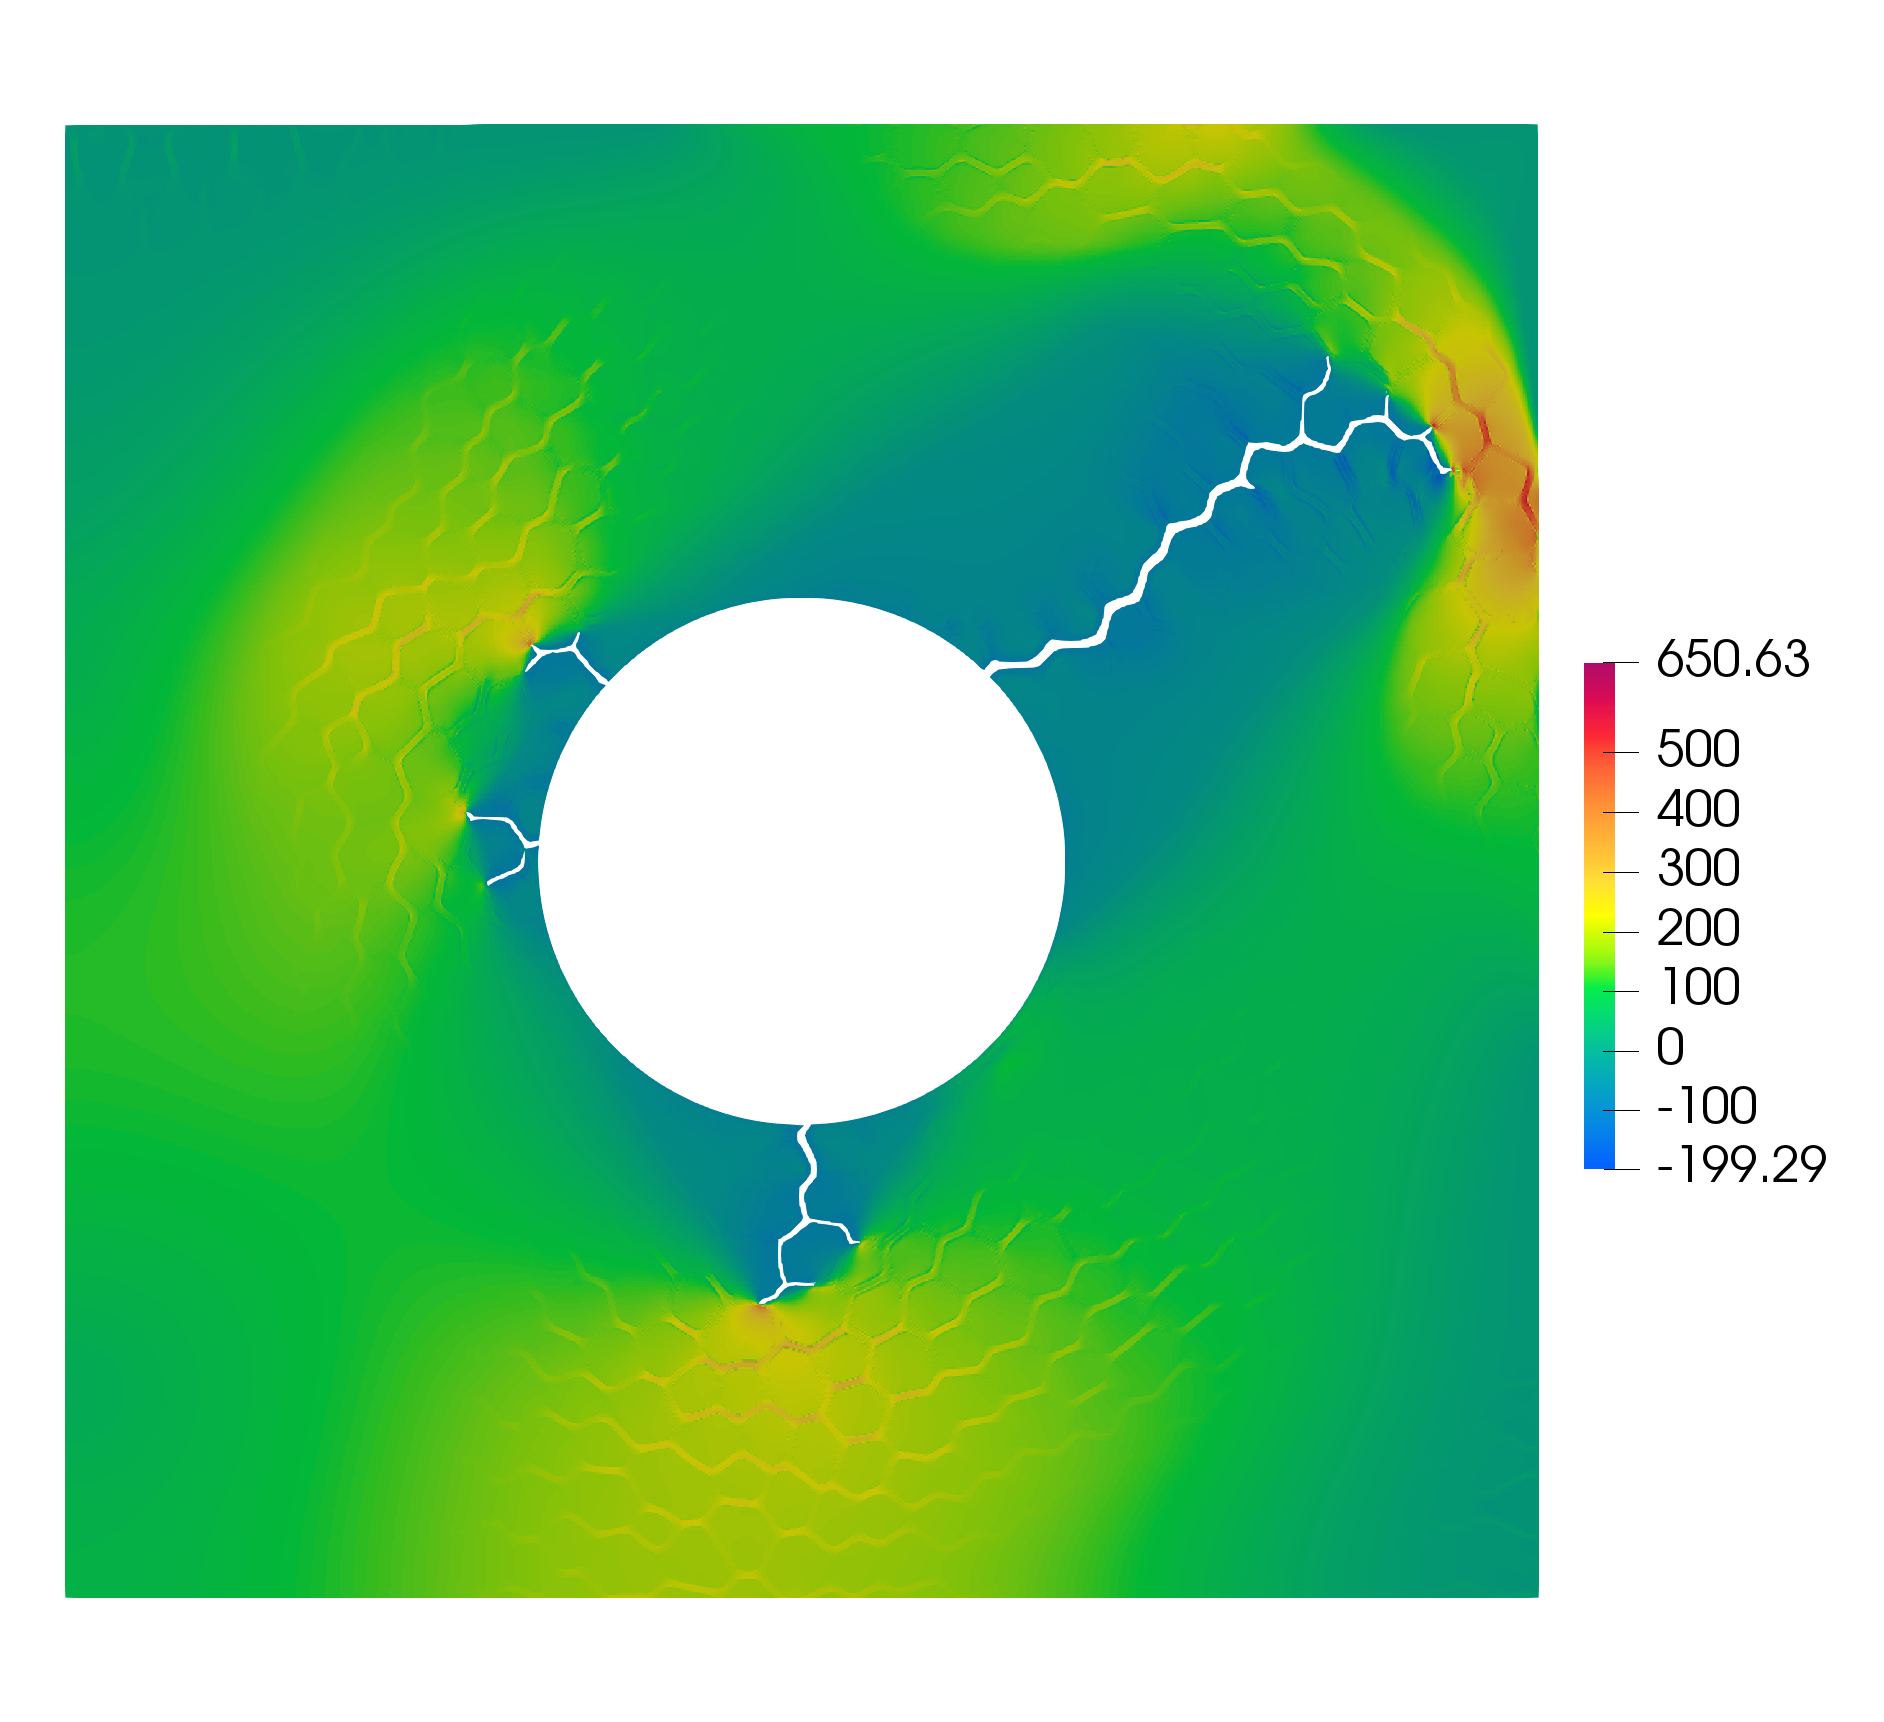
\includegraphics[width=\linewidth]{Chapter3/figures/r5_ext0_stress}
    \caption{}
  \end{subfigure}
  \caption{Results for (a-c) the small bubble with radius \SI{0.25}{\micro\meter} and (d-f) the large bubble with radius \SI{0.25}{\micro\meter} (a, d) Pressure history. (b, e) Crack paths superimposed on the voronoi structure. (c, f) Contour plot of the maximum principal stress.}
  \label{fig:r25}
\end{figure}

In a fuel pellet system, external pressure can arise from fuel-cladding mechanical interaction. To study the effect of external pressure, different external pressures are applied on the top and right boundaries.  The results from using three different external pressures, 0, \SI{30}{\mega\pascal}, \SI{60}{\mega\pascal}, are shown in \Cref{fig:compare_external_pressure}. The critical pressure is significantly higher for larger external pressure values, while there is no qualitative change in the crack pattern.

\begin{figure}[htb!]
  \centering
  \begin{subfigure}[t]{0.32\linewidth}
    \centering
    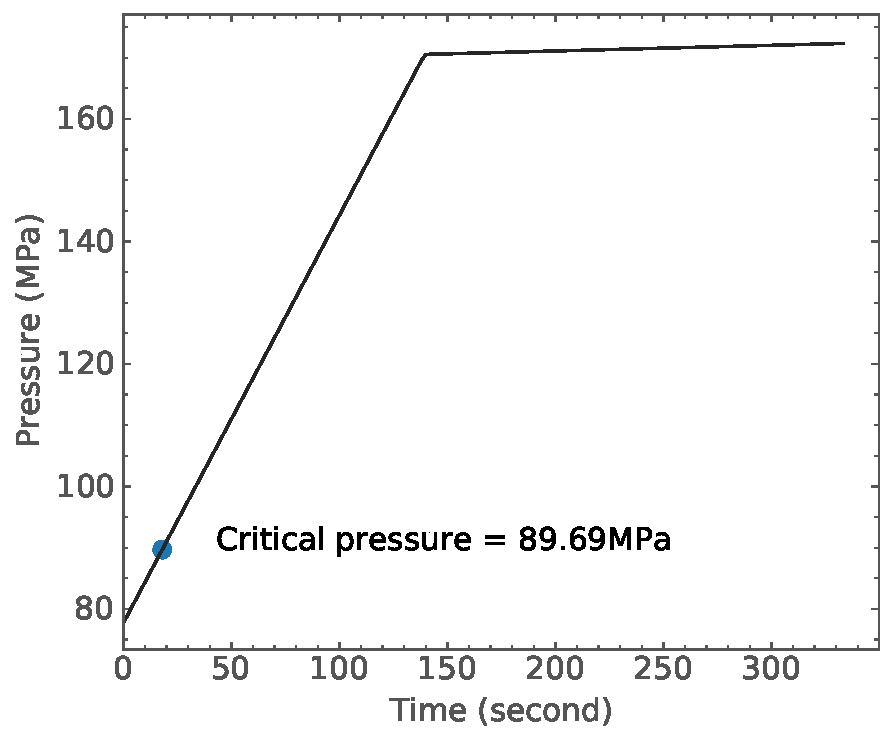
\includegraphics[width=\linewidth]{Chapter3/figures/bubble_pressure_r0.5_ext0_rod196}
    \caption{}
  \end{subfigure}
  \begin{subfigure}[t]{0.32\linewidth}
    \centering
    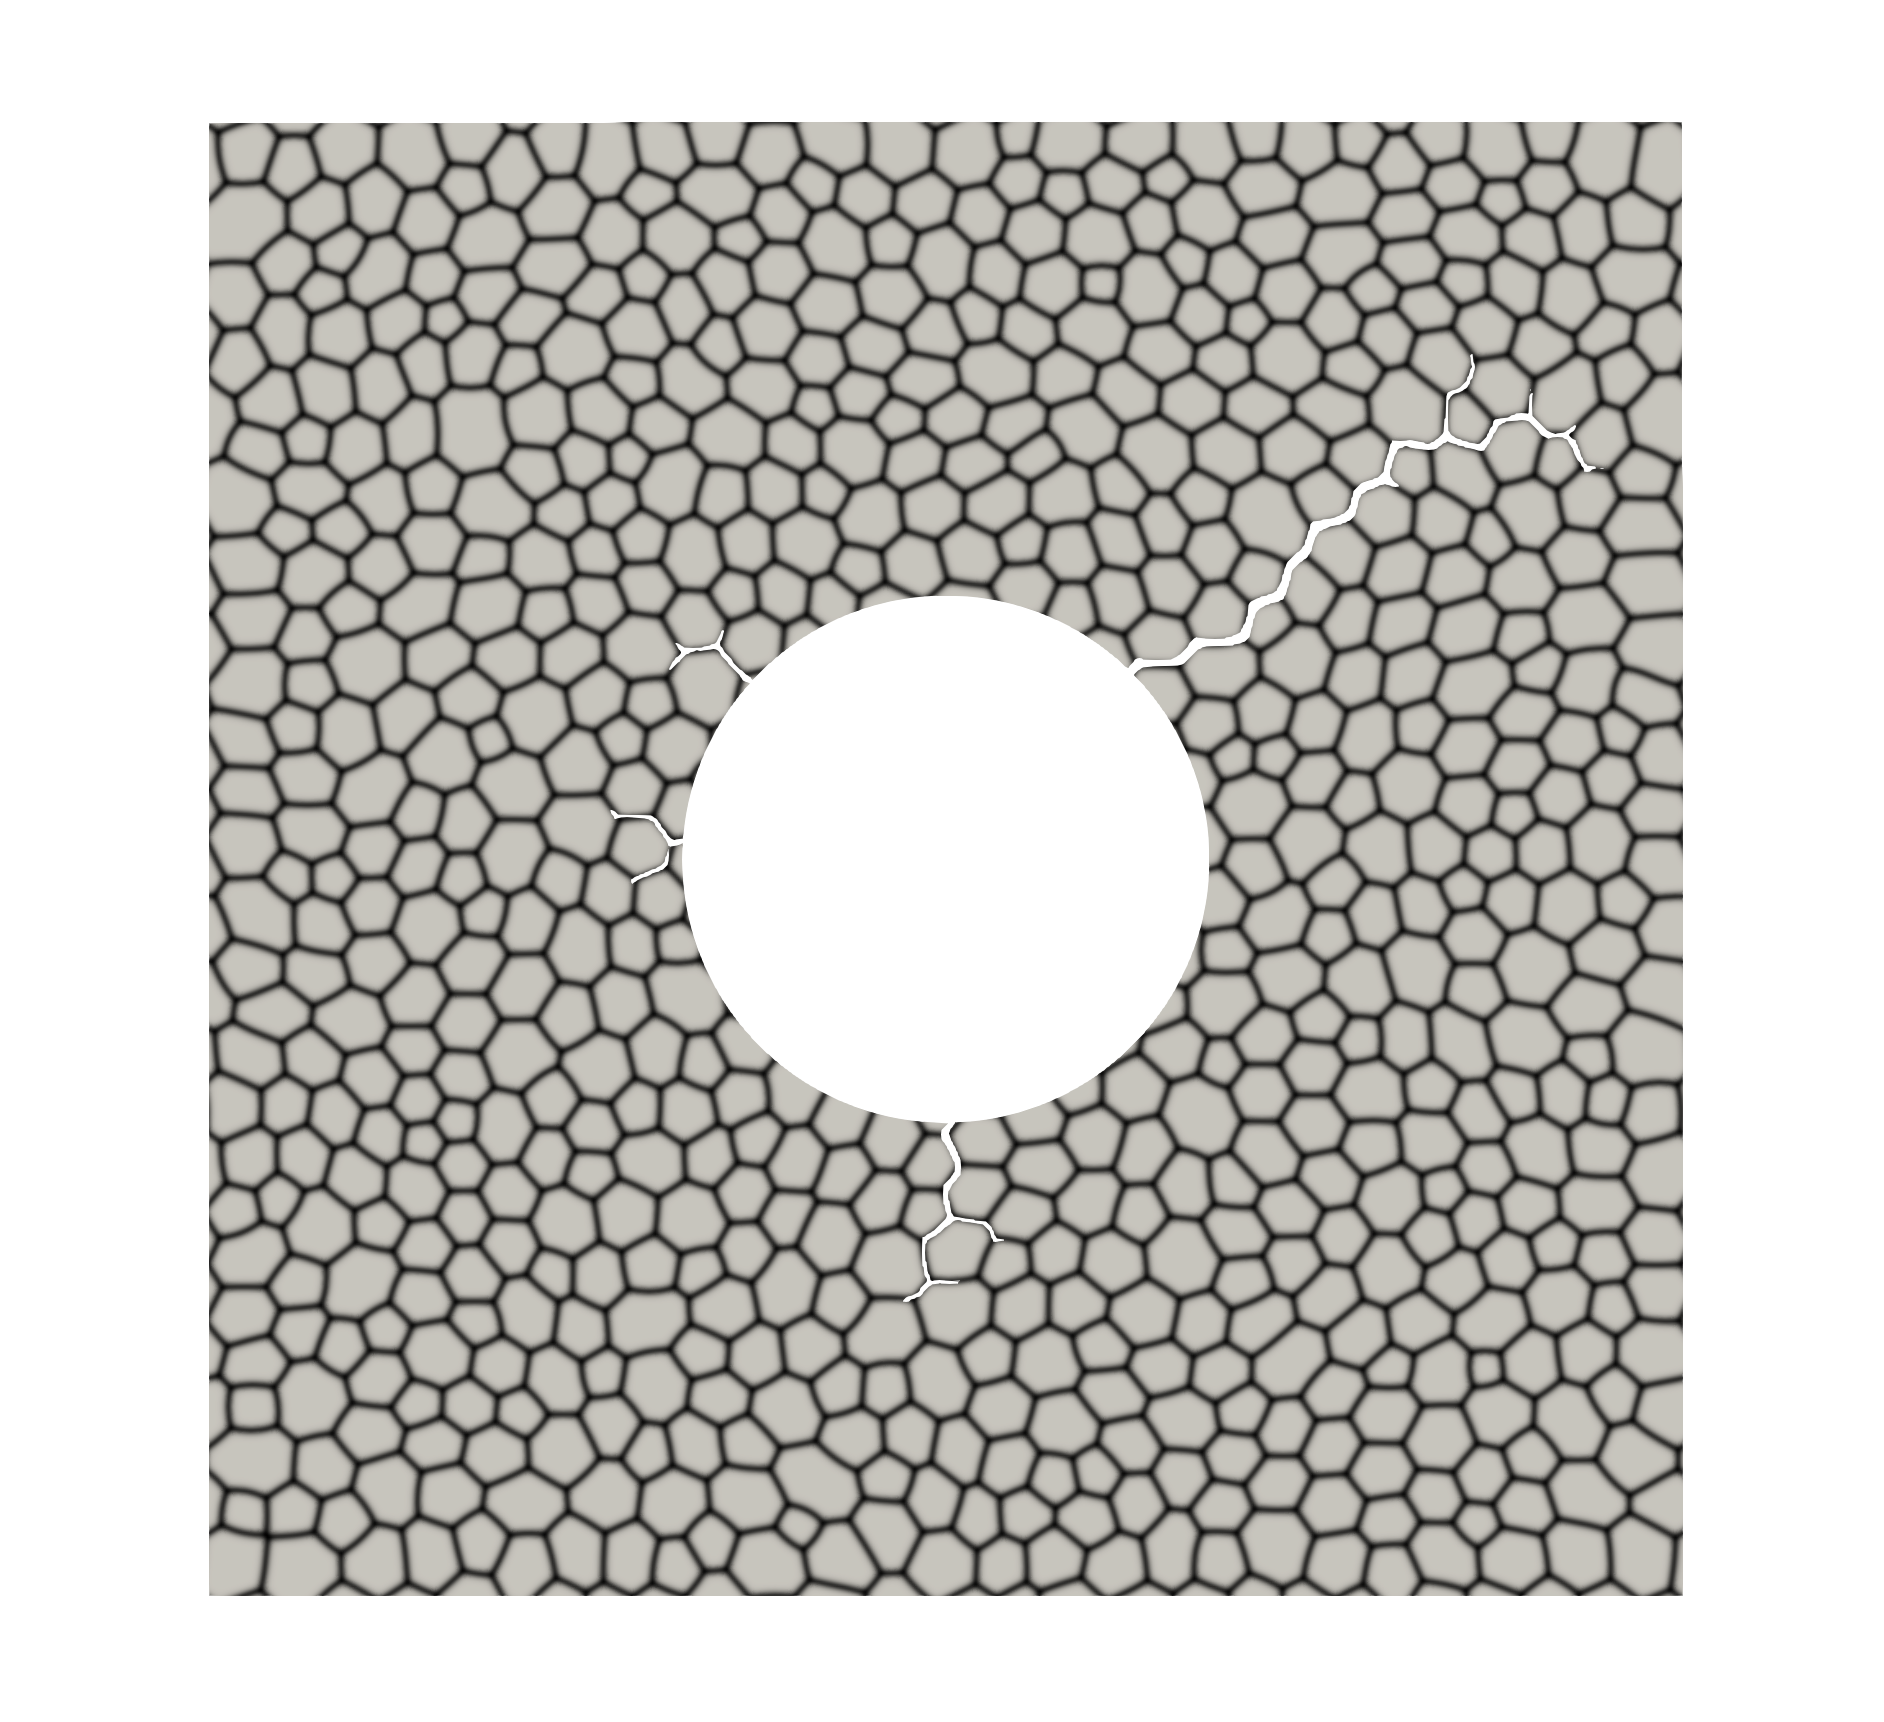
\includegraphics[width=\linewidth]{Chapter3/figures/r5_ext0}
    \caption{}
  \end{subfigure}
  \begin{subfigure}[t]{0.32\linewidth}
    \centering
    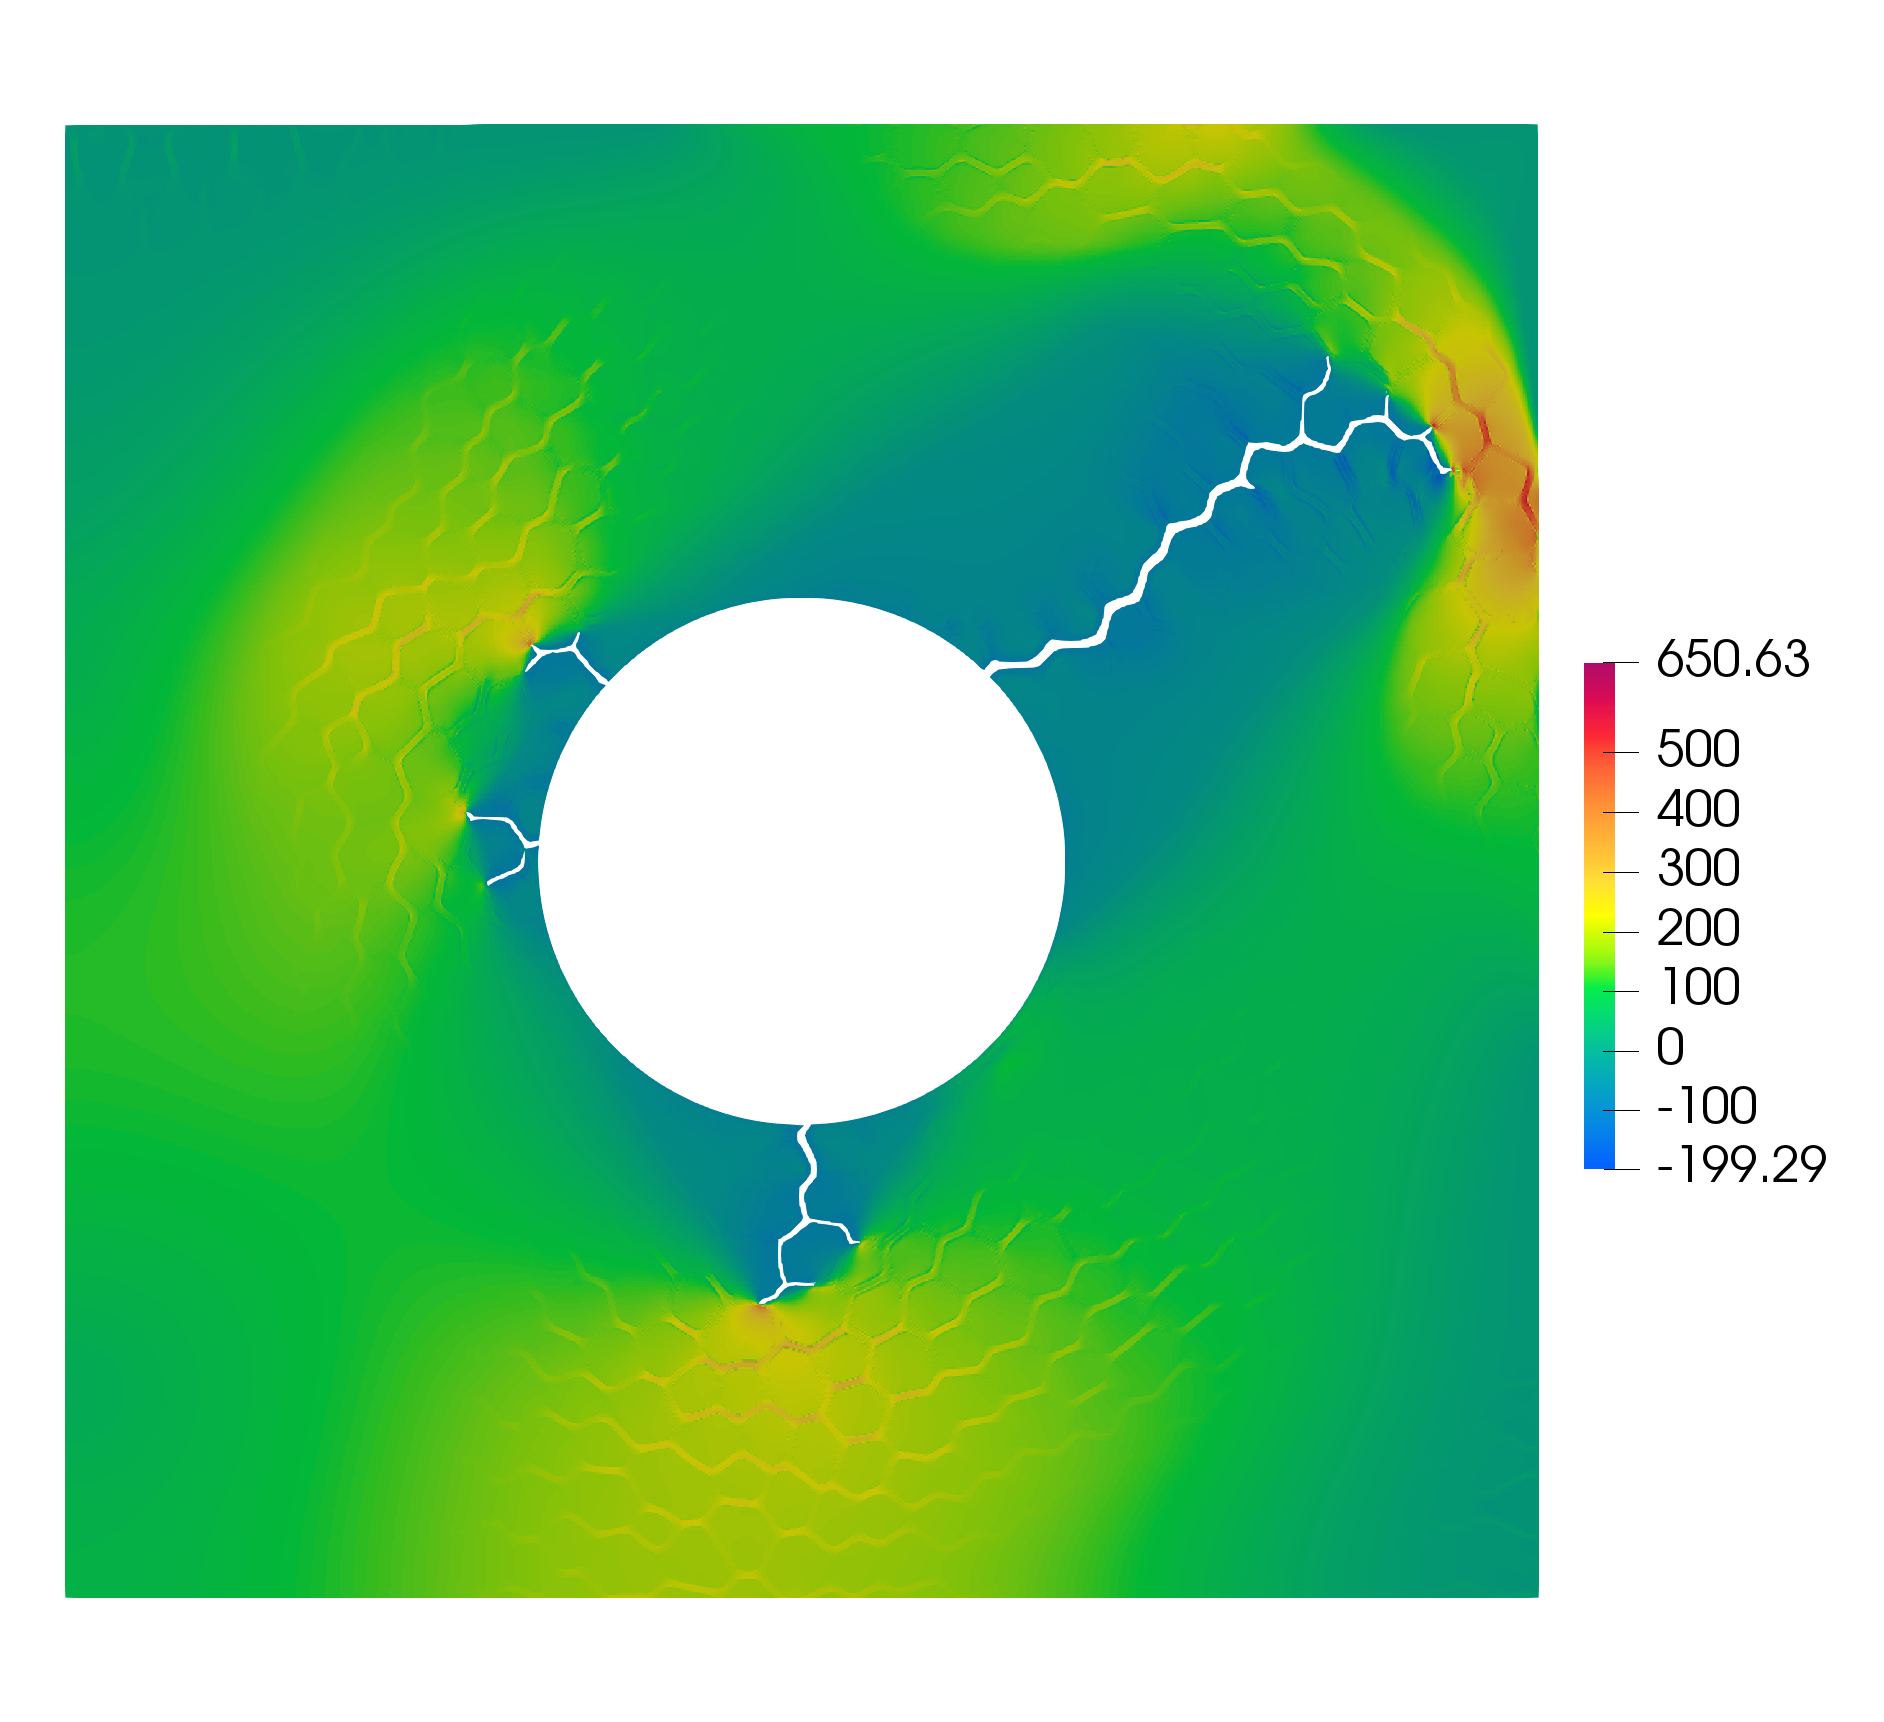
\includegraphics[width=\linewidth]{Chapter3/figures/r5_ext0_stress}
    \caption{}
  \end{subfigure}\\
  \begin{subfigure}[t]{0.32\linewidth}
    \centering
    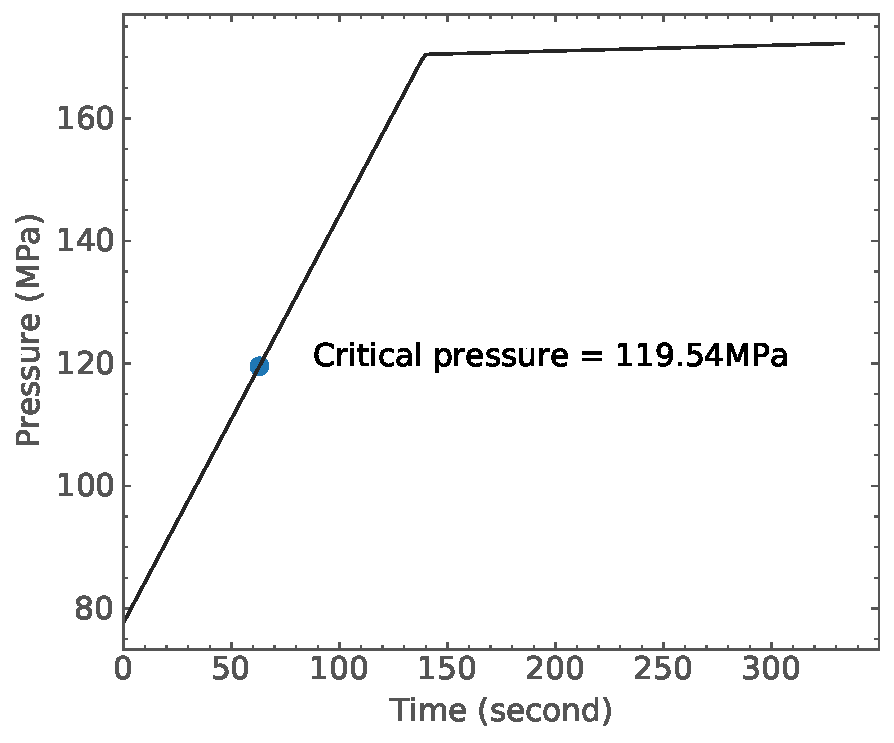
\includegraphics[width=\linewidth]{Chapter3/figures/bubble_pressure_r0.5_ext30_rod196}
    \caption{}
  \end{subfigure}
  \begin{subfigure}[t]{0.32\linewidth}
    \centering
    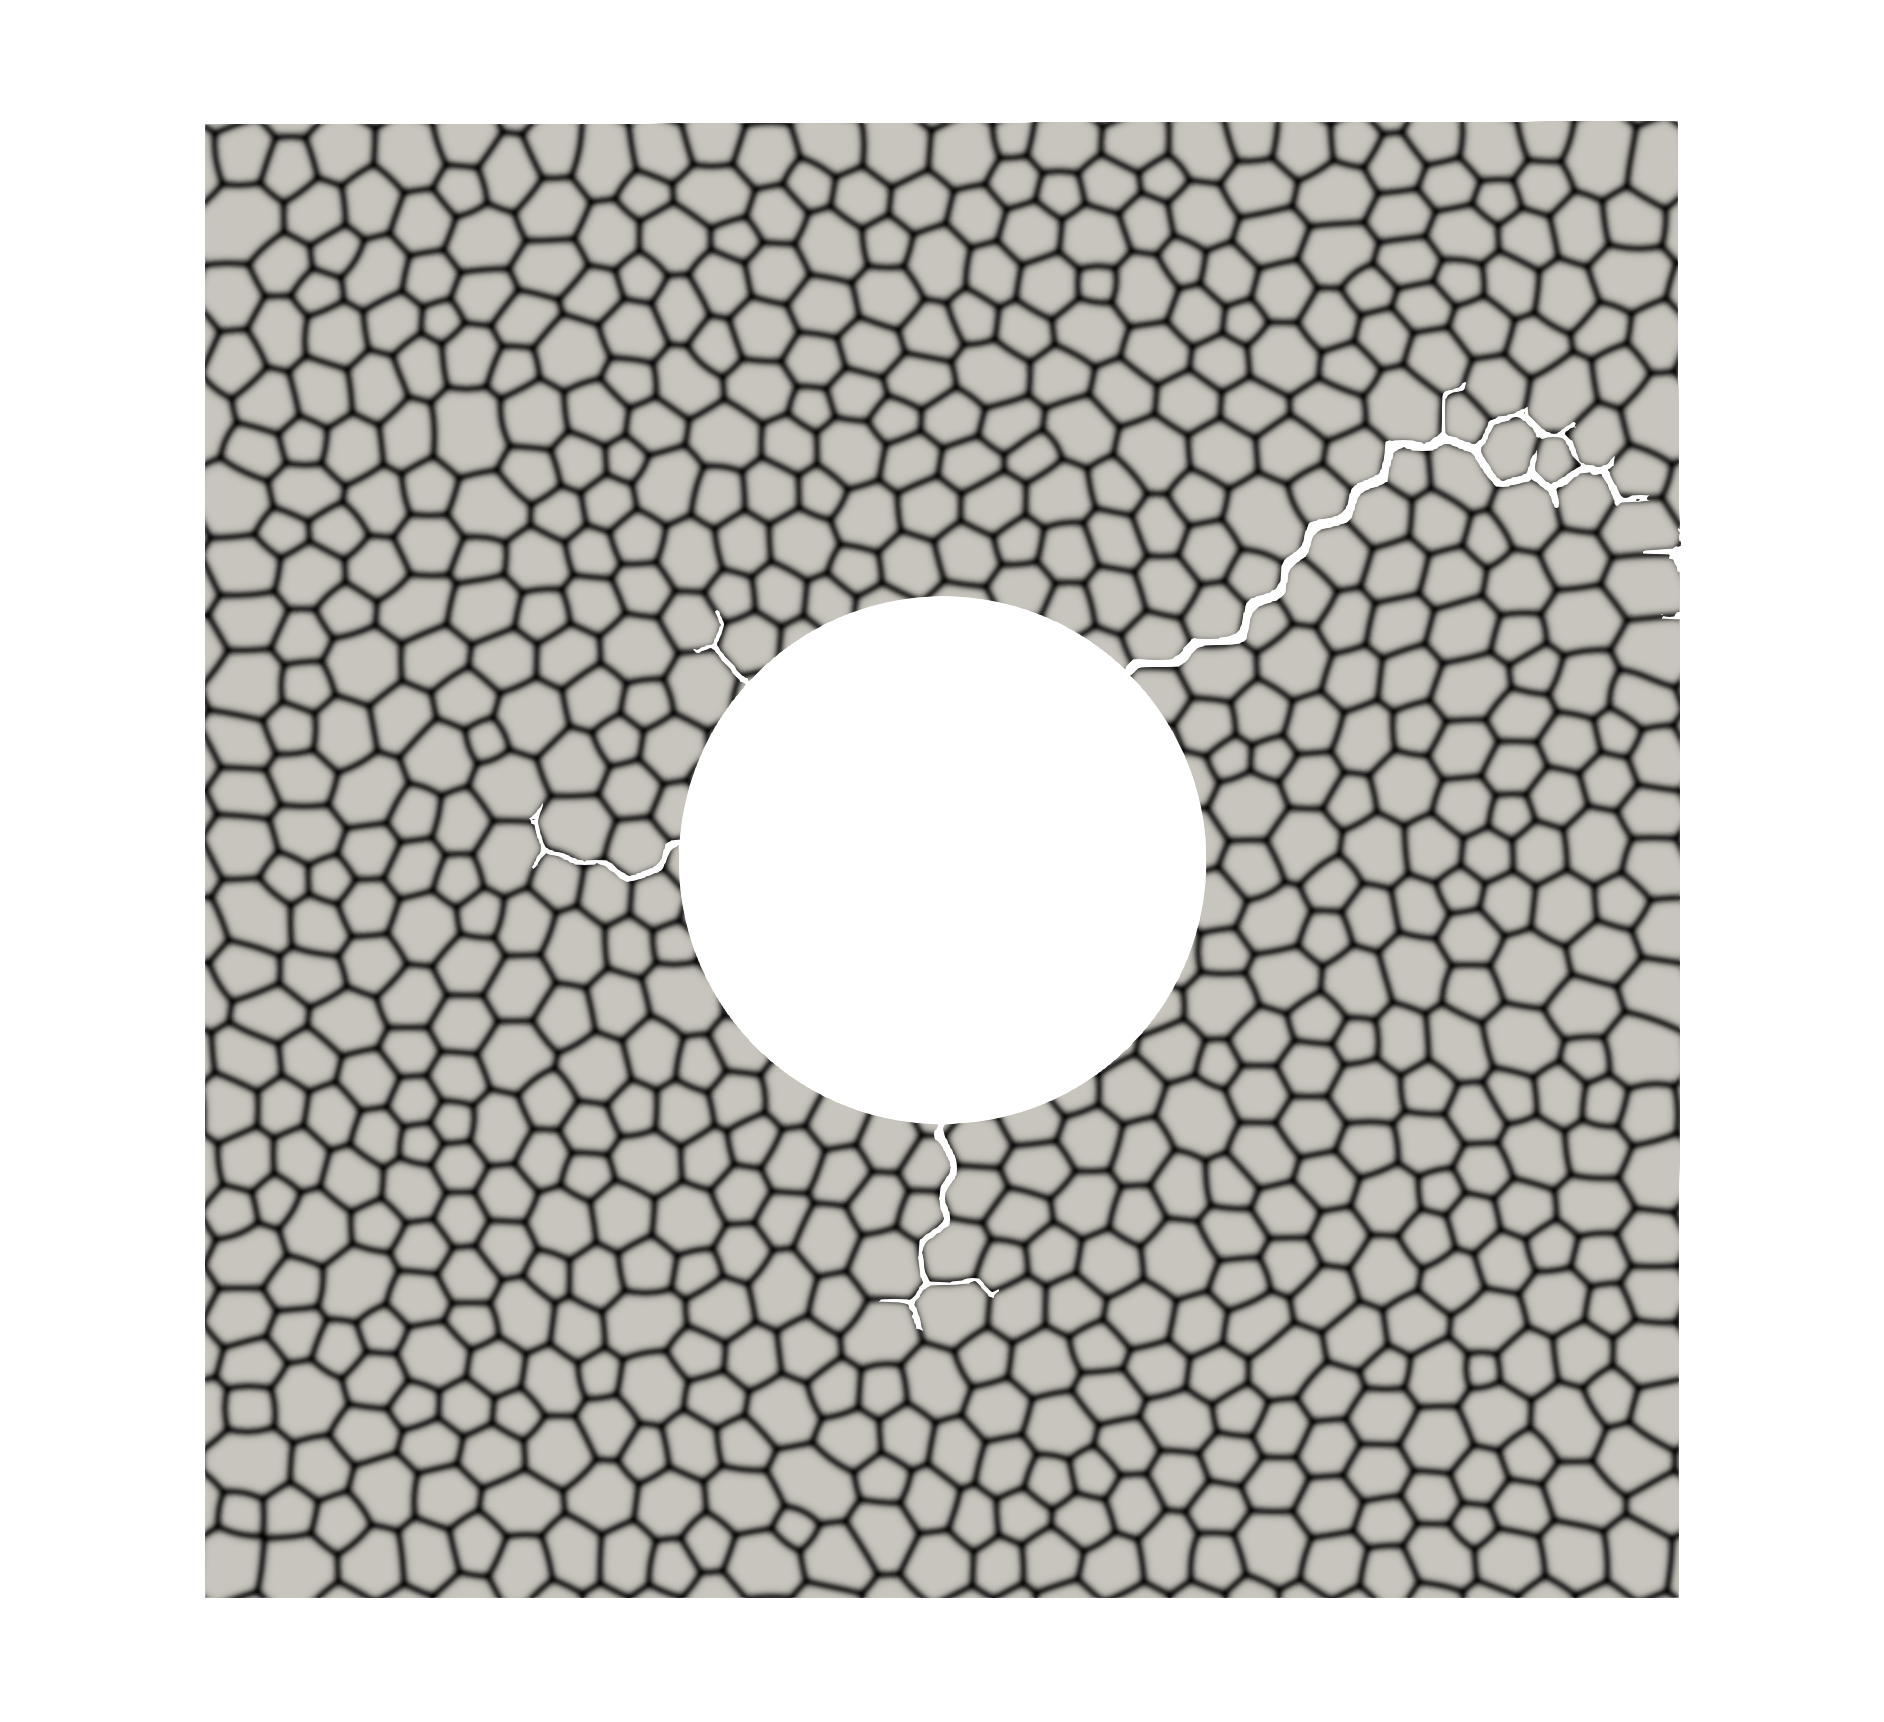
\includegraphics[width=\linewidth]{Chapter3/figures/r5_ext30}
    \caption{}
  \end{subfigure}
  \begin{subfigure}[t]{0.32\linewidth}
    \centering
    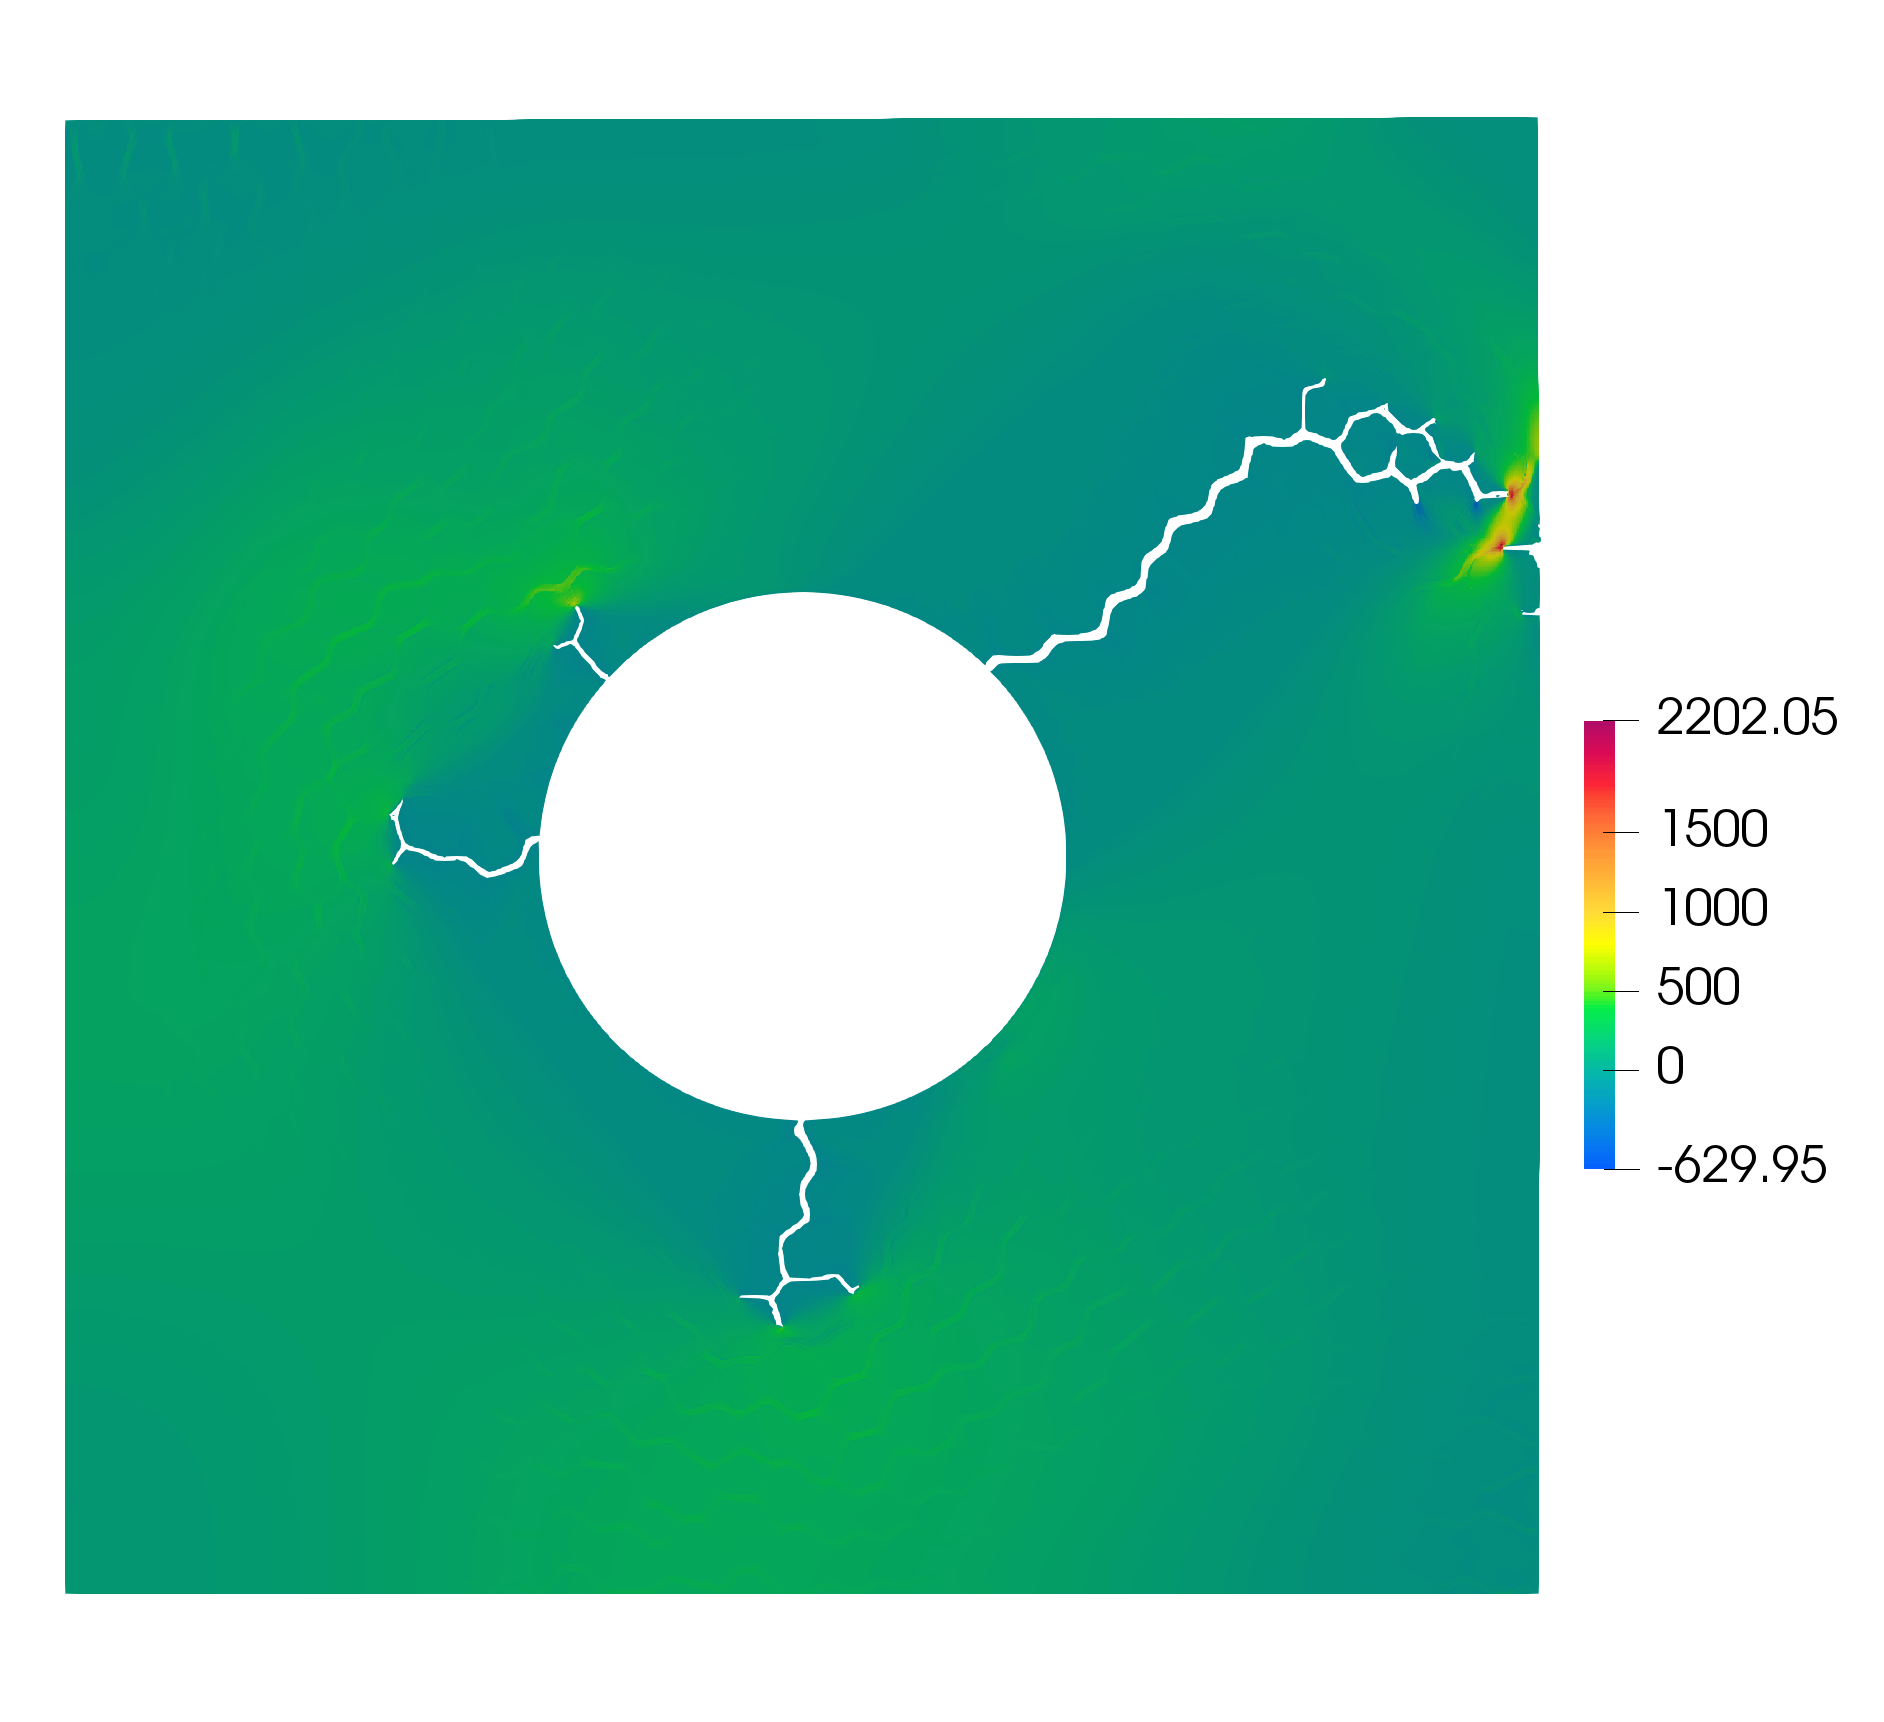
\includegraphics[width=\linewidth]{Chapter3/figures/r5_ext30_stress}
    \caption{}
  \end{subfigure}\\
  \begin{subfigure}[t]{0.32\linewidth}
    \centering
    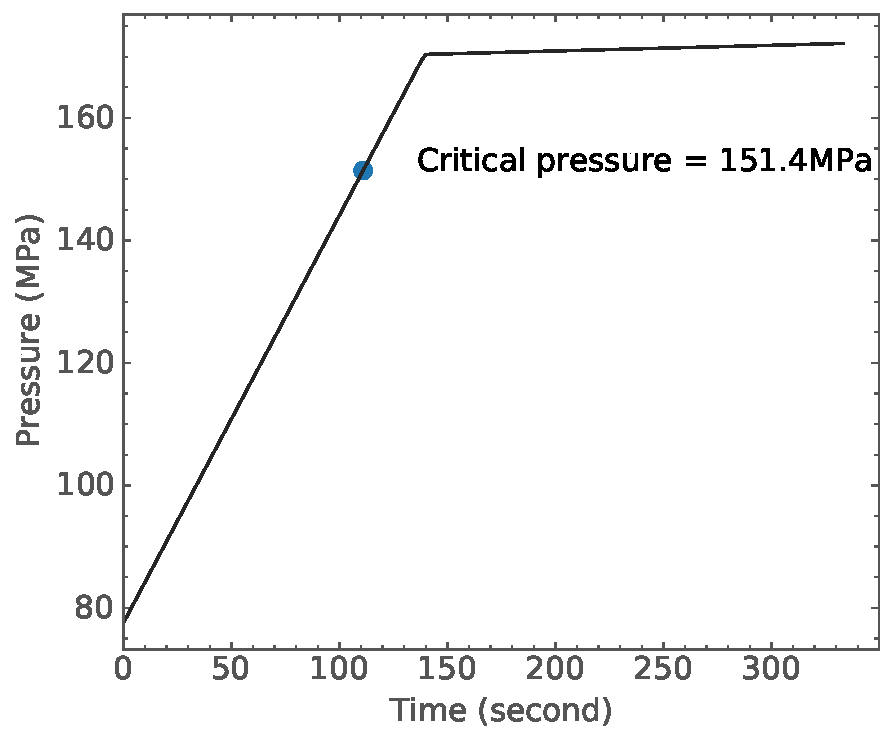
\includegraphics[width=\linewidth]{Chapter3/figures/bubble_pressure_r0.5_ext60_rod196}
    \caption{}
  \end{subfigure}
  \begin{subfigure}[t]{0.32\linewidth}
    \centering
    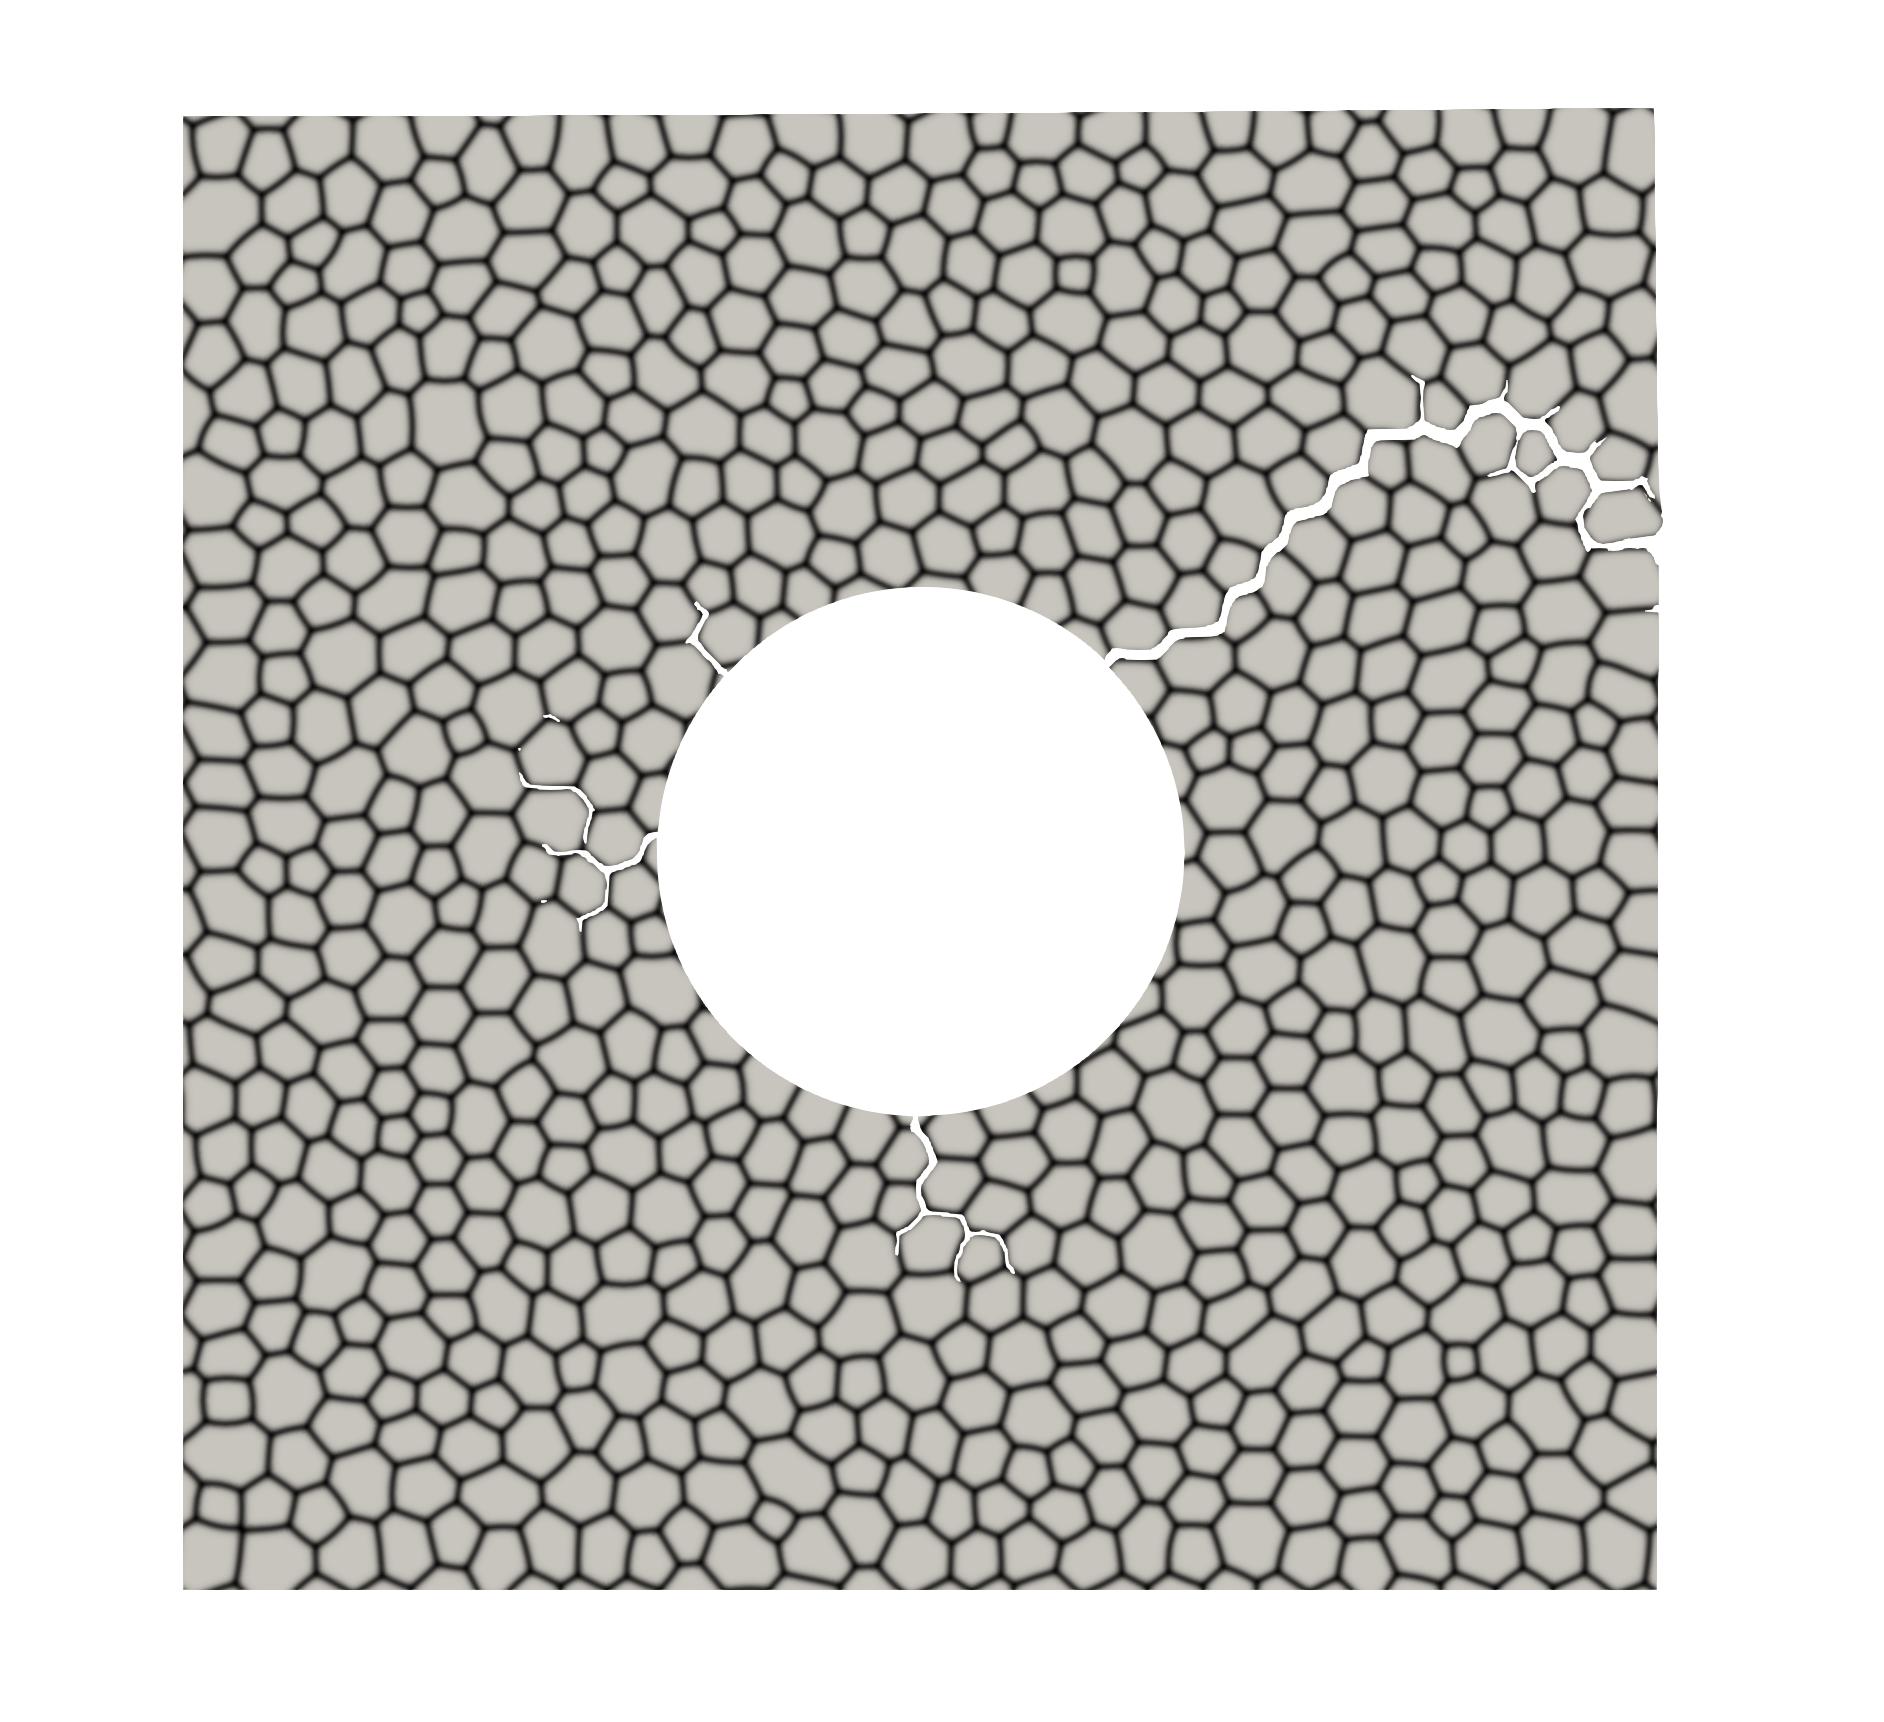
\includegraphics[width=\linewidth]{Chapter3/figures/r5_ext60}
    \caption{}
  \end{subfigure}
  \begin{subfigure}[t]{0.32\linewidth}
    \centering
    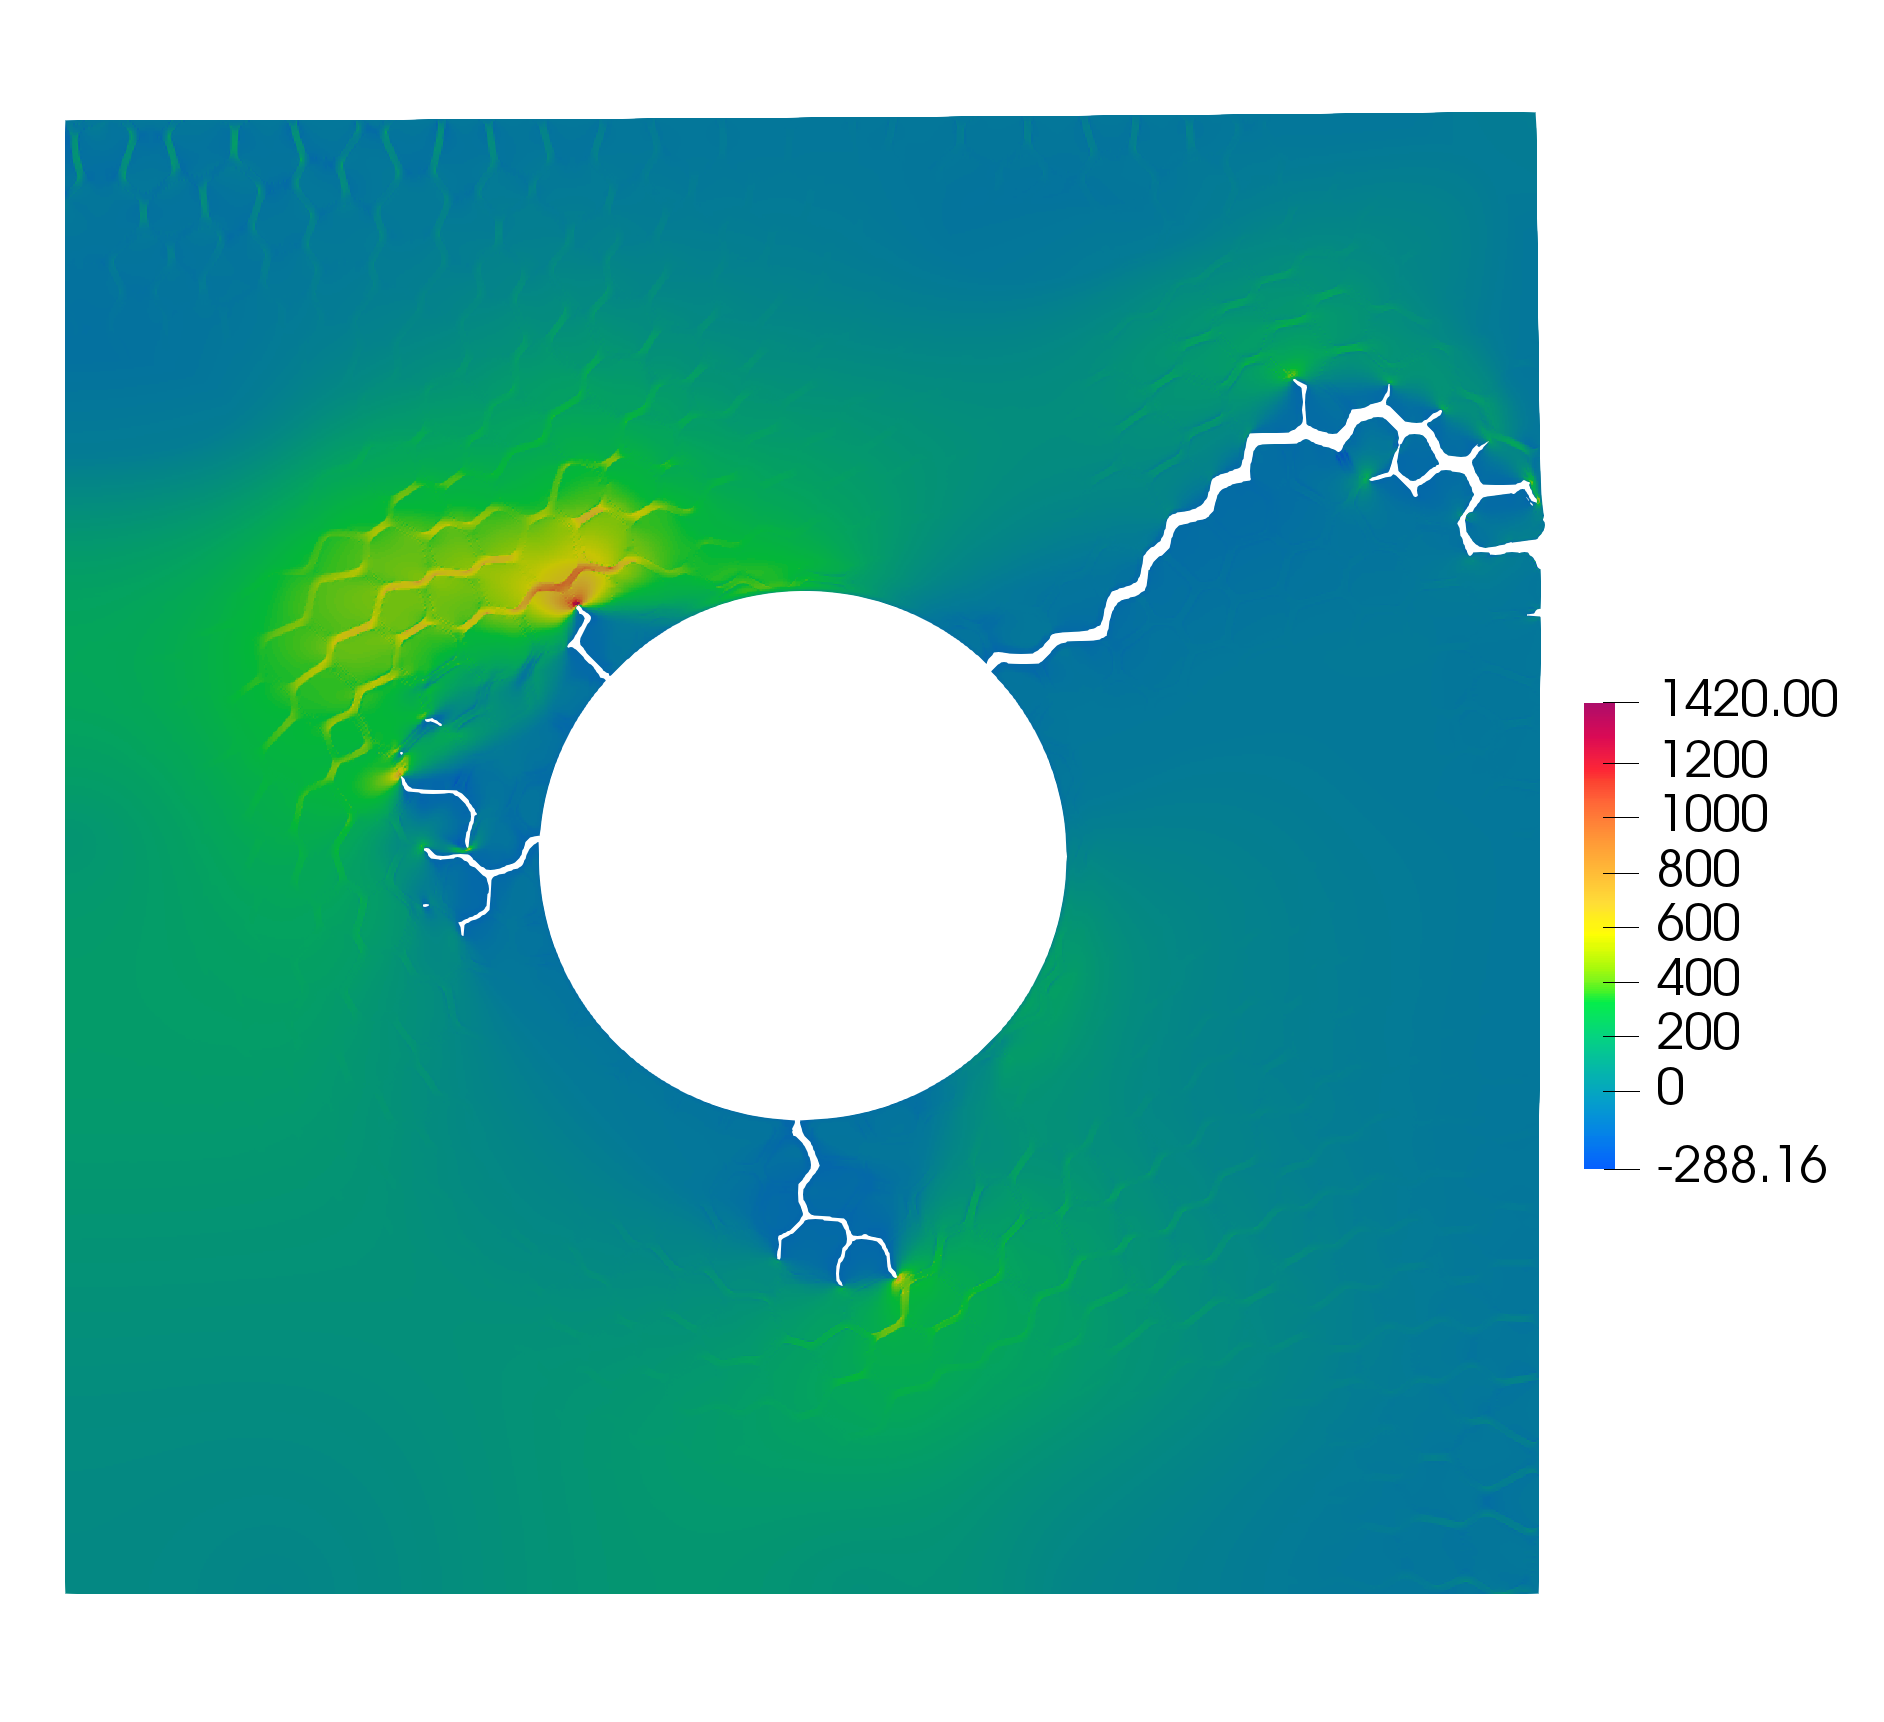
\includegraphics[width=\linewidth]{Chapter3/figures/r5_ext60_stress}
    \caption{}
  \end{subfigure}
  \caption{ Results for bubble radius \SI{0.5}{\micro\meter} and external pressure (a-c) \SI{0}{\mega\pascal}, (d-f) \SI{30}{\mega\pascal}, (g-i) \SI{60}{\mega\pascal}. (a, d, g) Pressure history. (b, e, h) Crack paths superimposed on the voronoi structure. (c, f, i) Contour plot of the maximum principal stress. }
  \label{fig:compare_external_pressure}
\end{figure}

%%%%%%%%%%%%%%%%%%%%%%%%%%%%%%%%%%%%%%%%%%%%%%%%%%%%%%%%%%%%%%%%%%%%%%%%%%%%%%%%%%%%%%%%%%%
%%%%%%%%%%%%%%%%%%%%%%%%%%%%%%%%%%%%%%%%%%%%%%%%%%%%%%%%%%%%%%%%%%%%%%%%%%%%%%%%%%%%%%%%%%%
%%%%%%%%%%%%%%%%%%%%%%%%%%%%%%%%%%%%%%%%%%%%%%%%%%%%%%%%%%%%%%%%%%%%%%%%%%%%%%%%%%%%%%%%%%%
%%%%%%%%%%%%%%%%%%%%%%%%%%%%%%%%%%%%%%%%%%%%%%%%%%%%%%%%%%%%%%%%%%%%%%%%%%%%%%%%%%%%%%%%%%%
%%%%%%%%%%%%%%%%%%%%%%%%%%%%%%%%%%%%%%%%%%%%%%%%%%%%%%%%%%%%%%%%%%%%%%%%%%%%%%%%%%%%%%%%%%%
%%%%%%%%%%%%%%%%%%%%%%%%%%%%%%%%%%%%%%%%%%%%%%%%%%%%%%%%%%%%%%%%%%%%%%%%%%%%%%%%%%%%%%%%%%%
%%%%%%%%%%%%%%%%%%%%%%%%%%%%%%%%%%%%%%%%%%%%%%%%%%%%%%%%%%%%%%%%%%%%%%%%%%%%%%%%%%%%%%%%%%%
%%%%%%%%%%%%%%%%%%%%%%%%%%%%%%%%%%%%%%%%%%%%%%%%%%%%%%%%%%%%%%%%%%%%%%%%%%%%%%%%%%%%%%%%%%%
%%%%%%%%%%%%%%%%%%%%%%%%%%%%%%%%%%%%%%%%%%%%%%%%%%%%%%%%%%%%%%%%%%%%%%%%%%%%%%%%%%%%%%%%%%%
%%%%%%%%%%%%%%%%%%%%%%%%%%%%%%%%%%%%%%%%%%%%%%%%%%%%%%%%%%%%%%%%%%%%%%%%%%%%%%%%%%%%%%%%%%%
\subsubsection{Multi-bubble interaction}

We next investigate the effect of the spatial distribution of the gas bubbles on fragment size. To that end, dimensions are expressed in dimensionless form in this section. With the origin of the coordinate system placed at the lower left corner of the REV, two cases are considered:
\begin{itemize}
  \item Two bubbles with centers at $\left( \dfrac{2}{15}L, \dfrac{7}{15}L \right)$ and $\left( \dfrac{7}{15}L, \dfrac{2}{15}L \right)$.
  \item Three bubbles with centers at $\left( \dfrac{1}{6}L, \dfrac{8}{15}L \right)$, $\left( \dfrac{8}{15}L, \dfrac{1}{6}L \right)$, and $\left( \dfrac{8}{15}L, \dfrac{8}{15}L \right)$.
\end{itemize}
All bubbles have a radius of $\dfrac{1}{12}L$. Results are shown in \Cref{fig:compare_bubble_distribution}. It is observed that the crack paths in cases involving multiple bubbles is strongly affected by the positions of the bubbles relative to each other: Cracks prefer to connect neighboring bubbles. Fully developed cracks and bubbles form a fragment at the lower-left corner in both cases. These fragments consist of multiple grains, and their sizes are affected by the spatial distribution of bubbles.

\begin{figure}[htb!]
  \centering
  \begin{subfigure}[t]{0.4\linewidth}
    \centering
    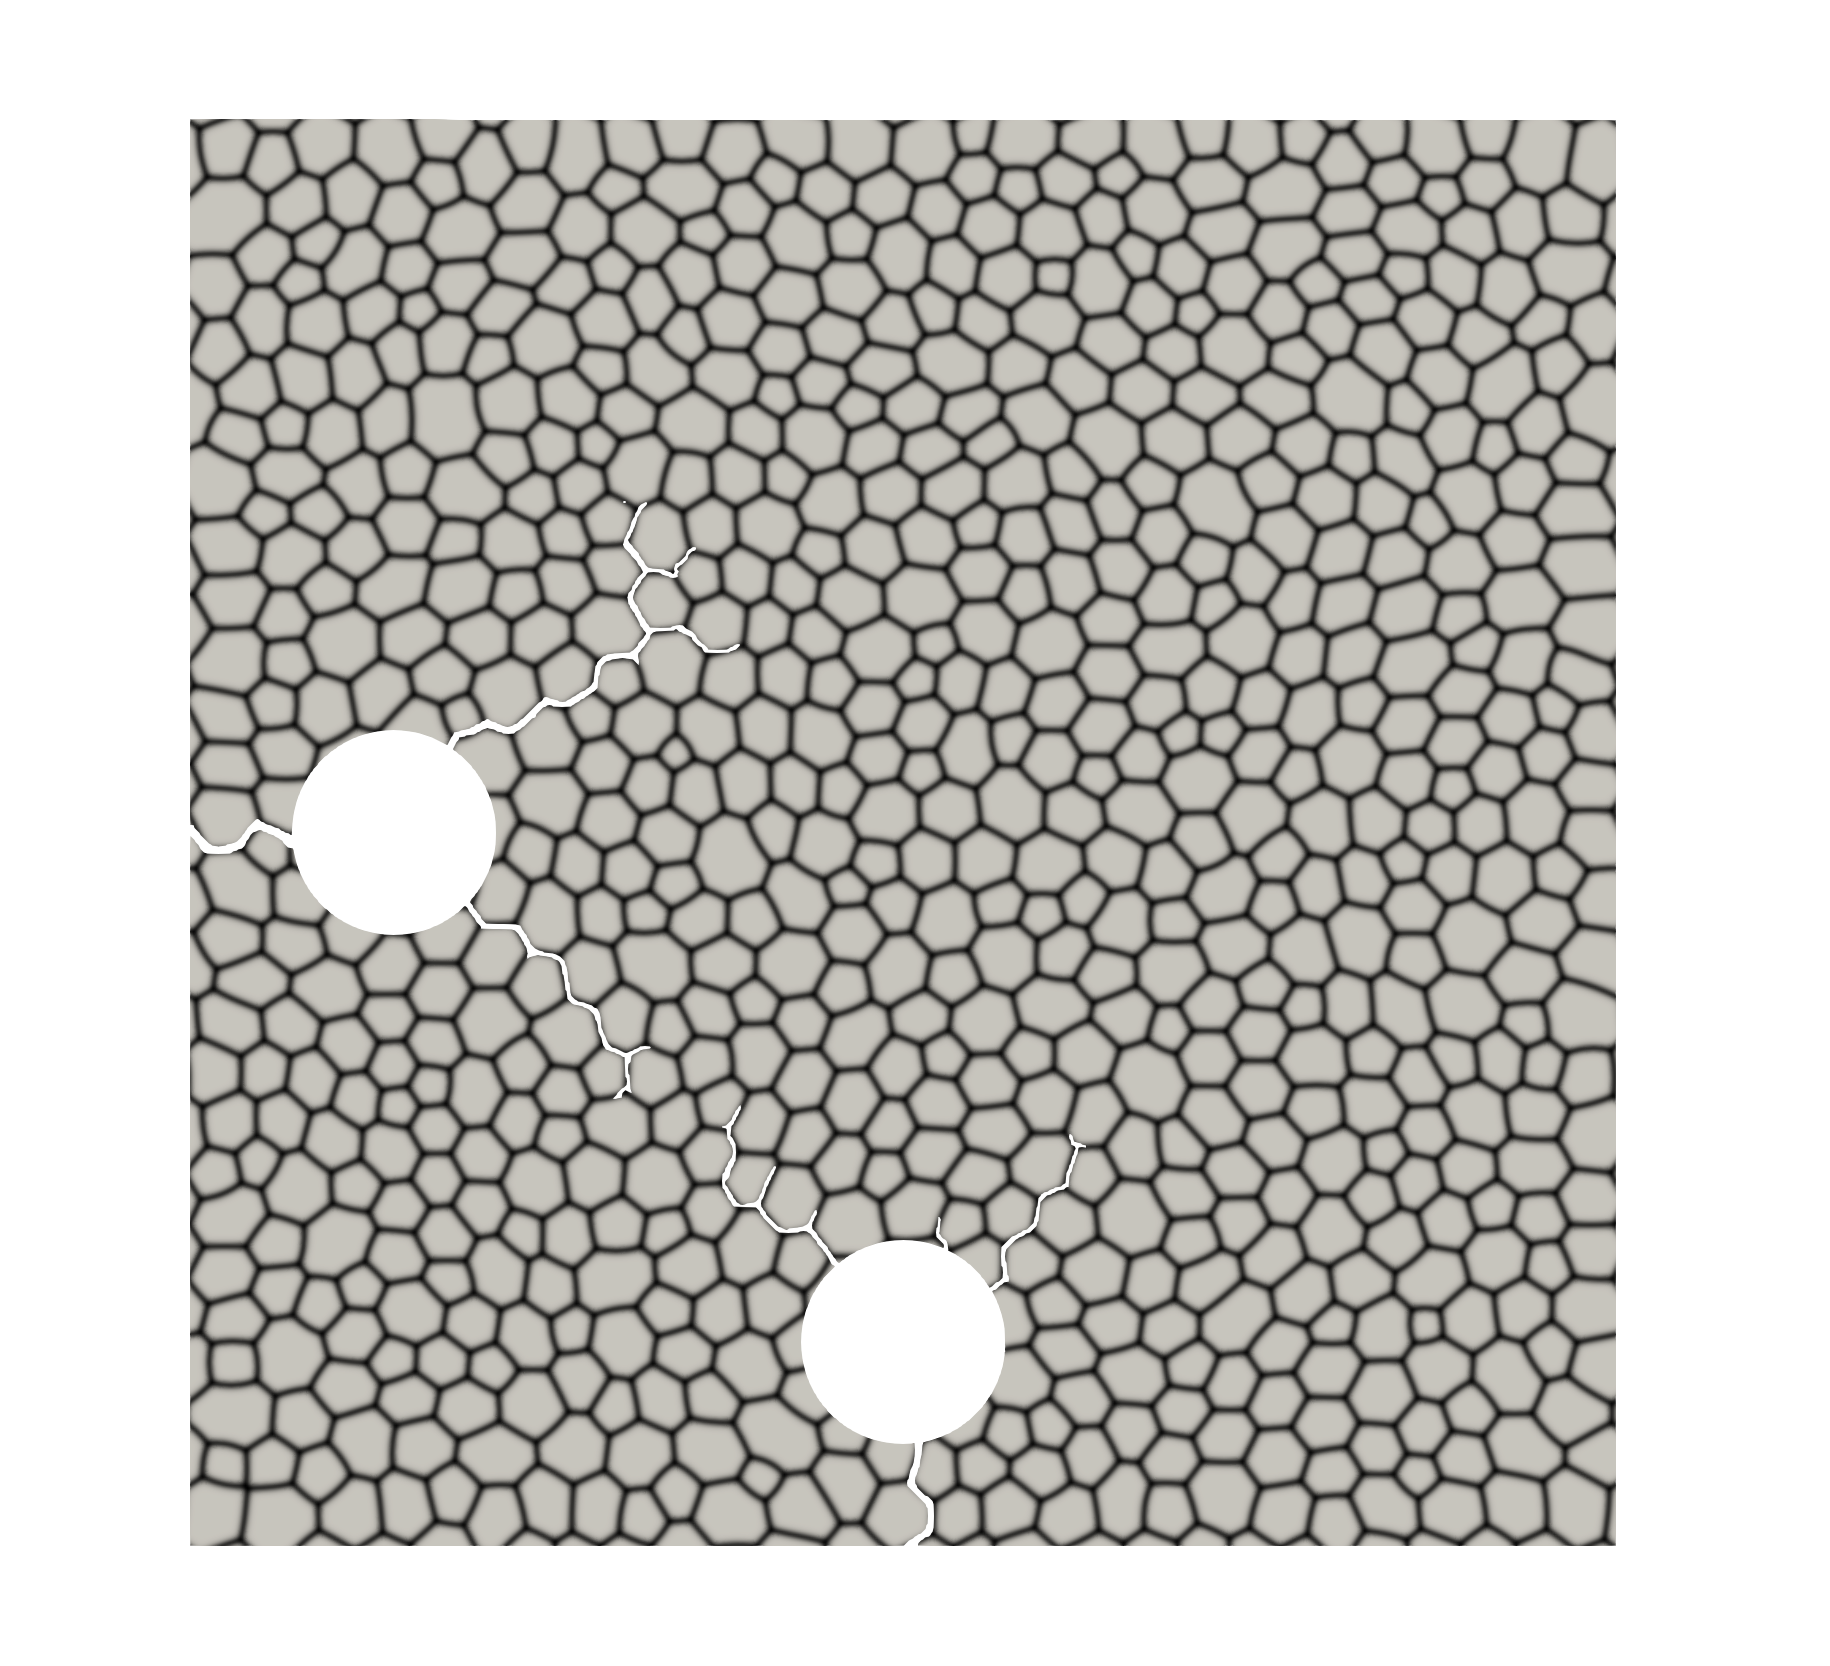
\includegraphics[width=\linewidth]{Chapter3/figures/two_bubbles_bnd}
    \caption{}
  \end{subfigure}
  \begin{subfigure}[t]{0.4\linewidth}
    \centering
    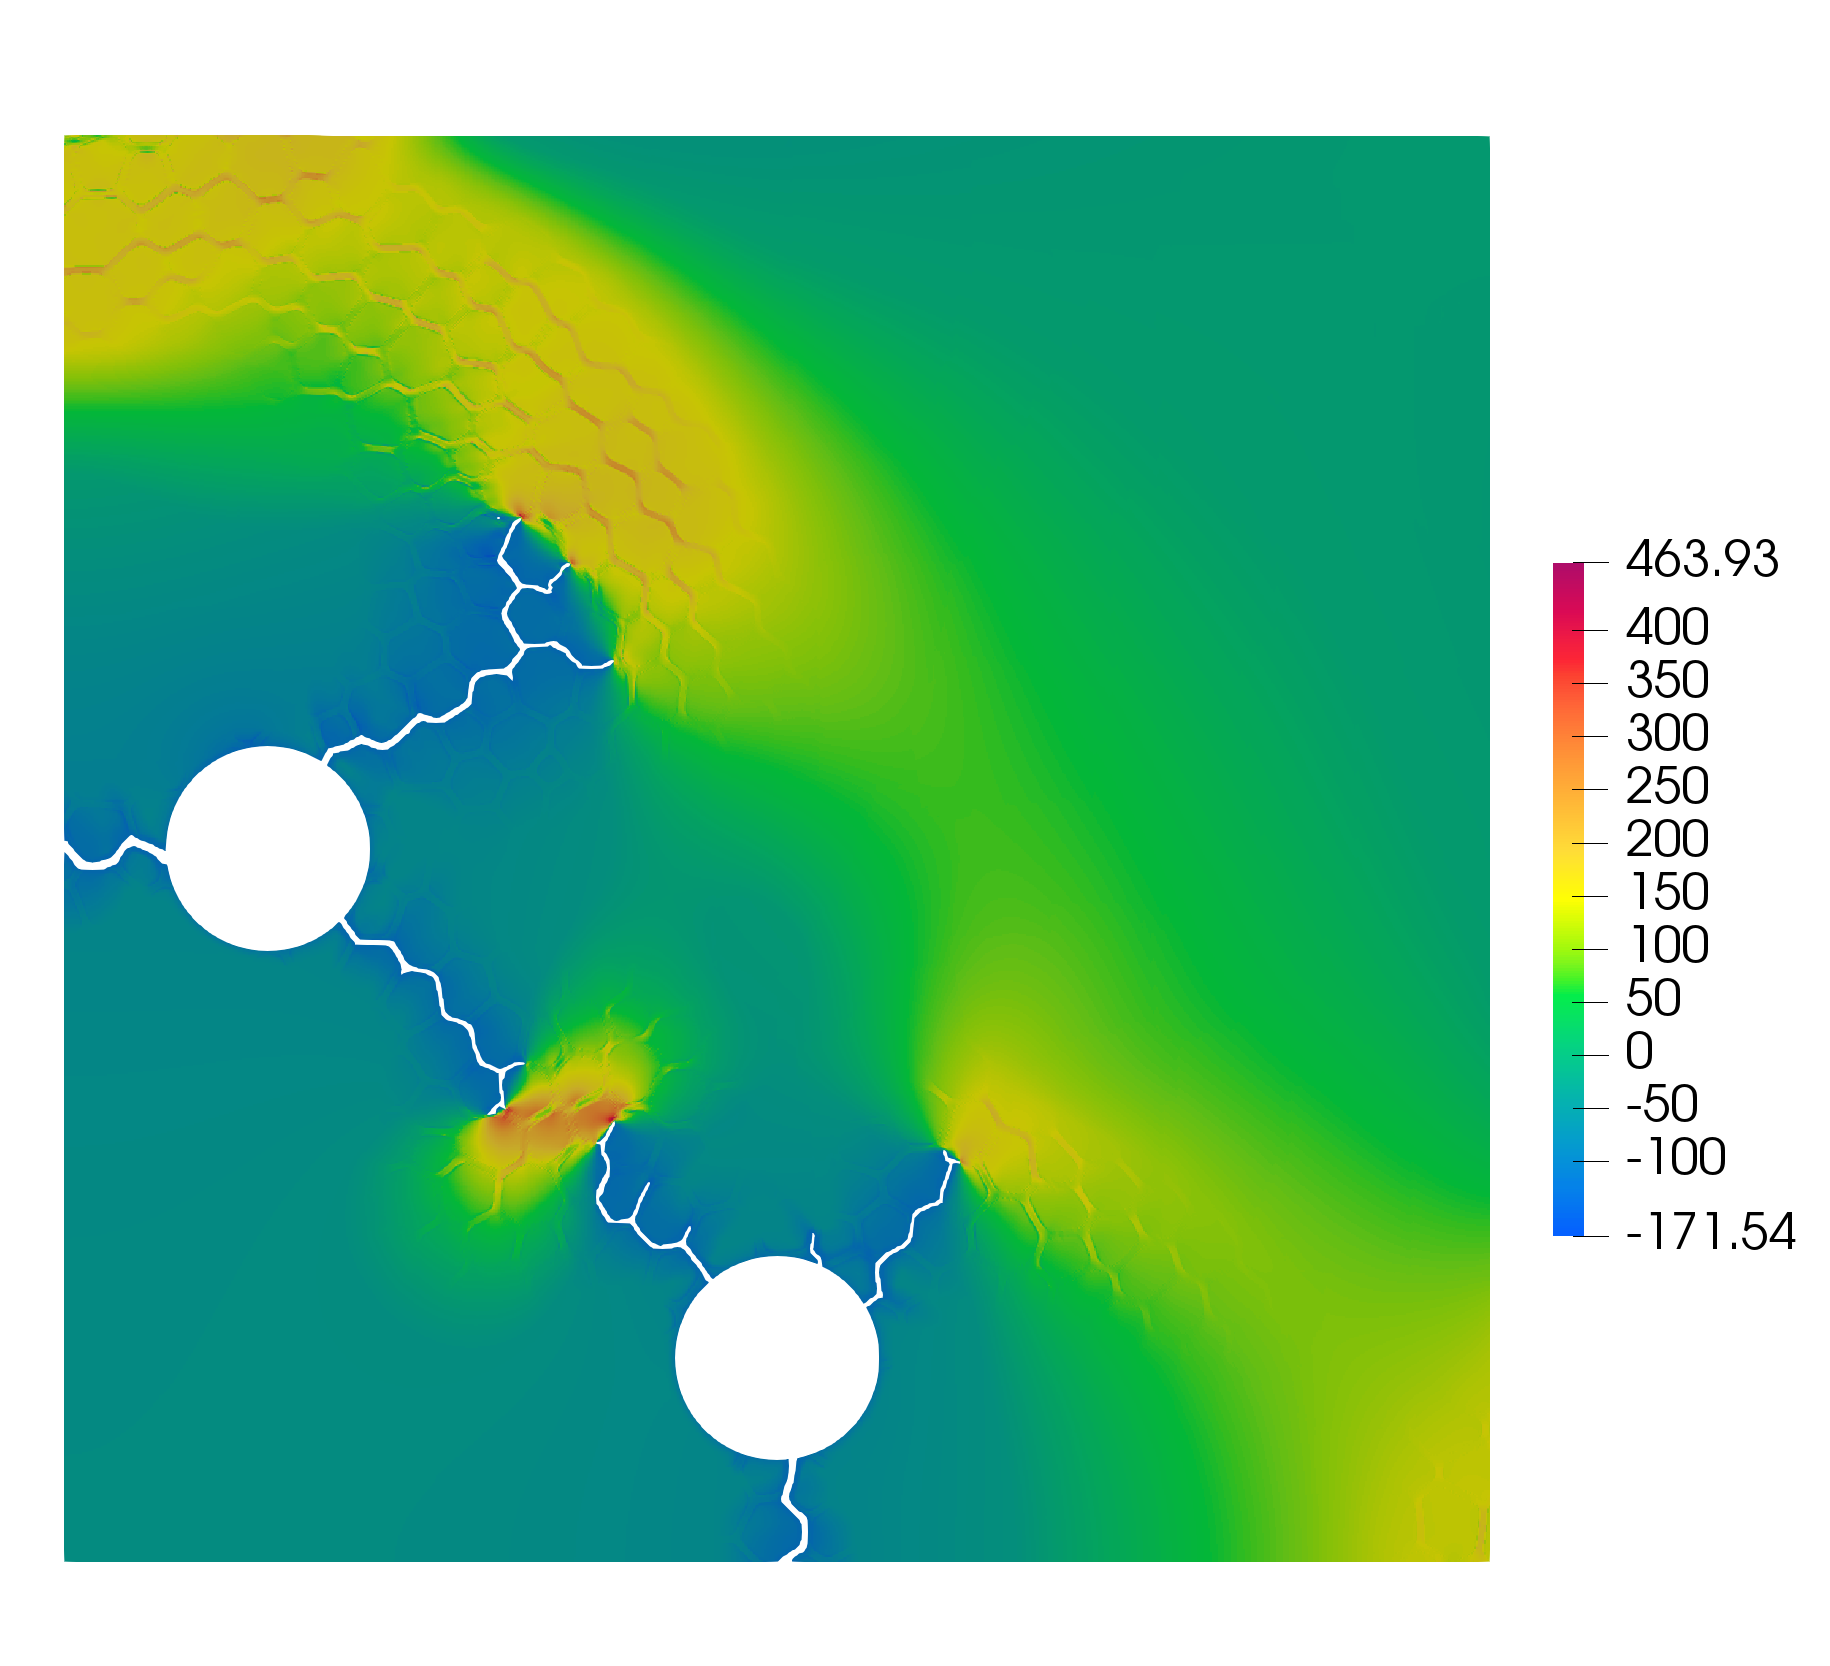
\includegraphics[width=\linewidth]{Chapter3/figures/two_bubbles_stress}
    \caption{}
  \end{subfigure} \\
  \begin{subfigure}[t]{0.4\linewidth}
    \centering
    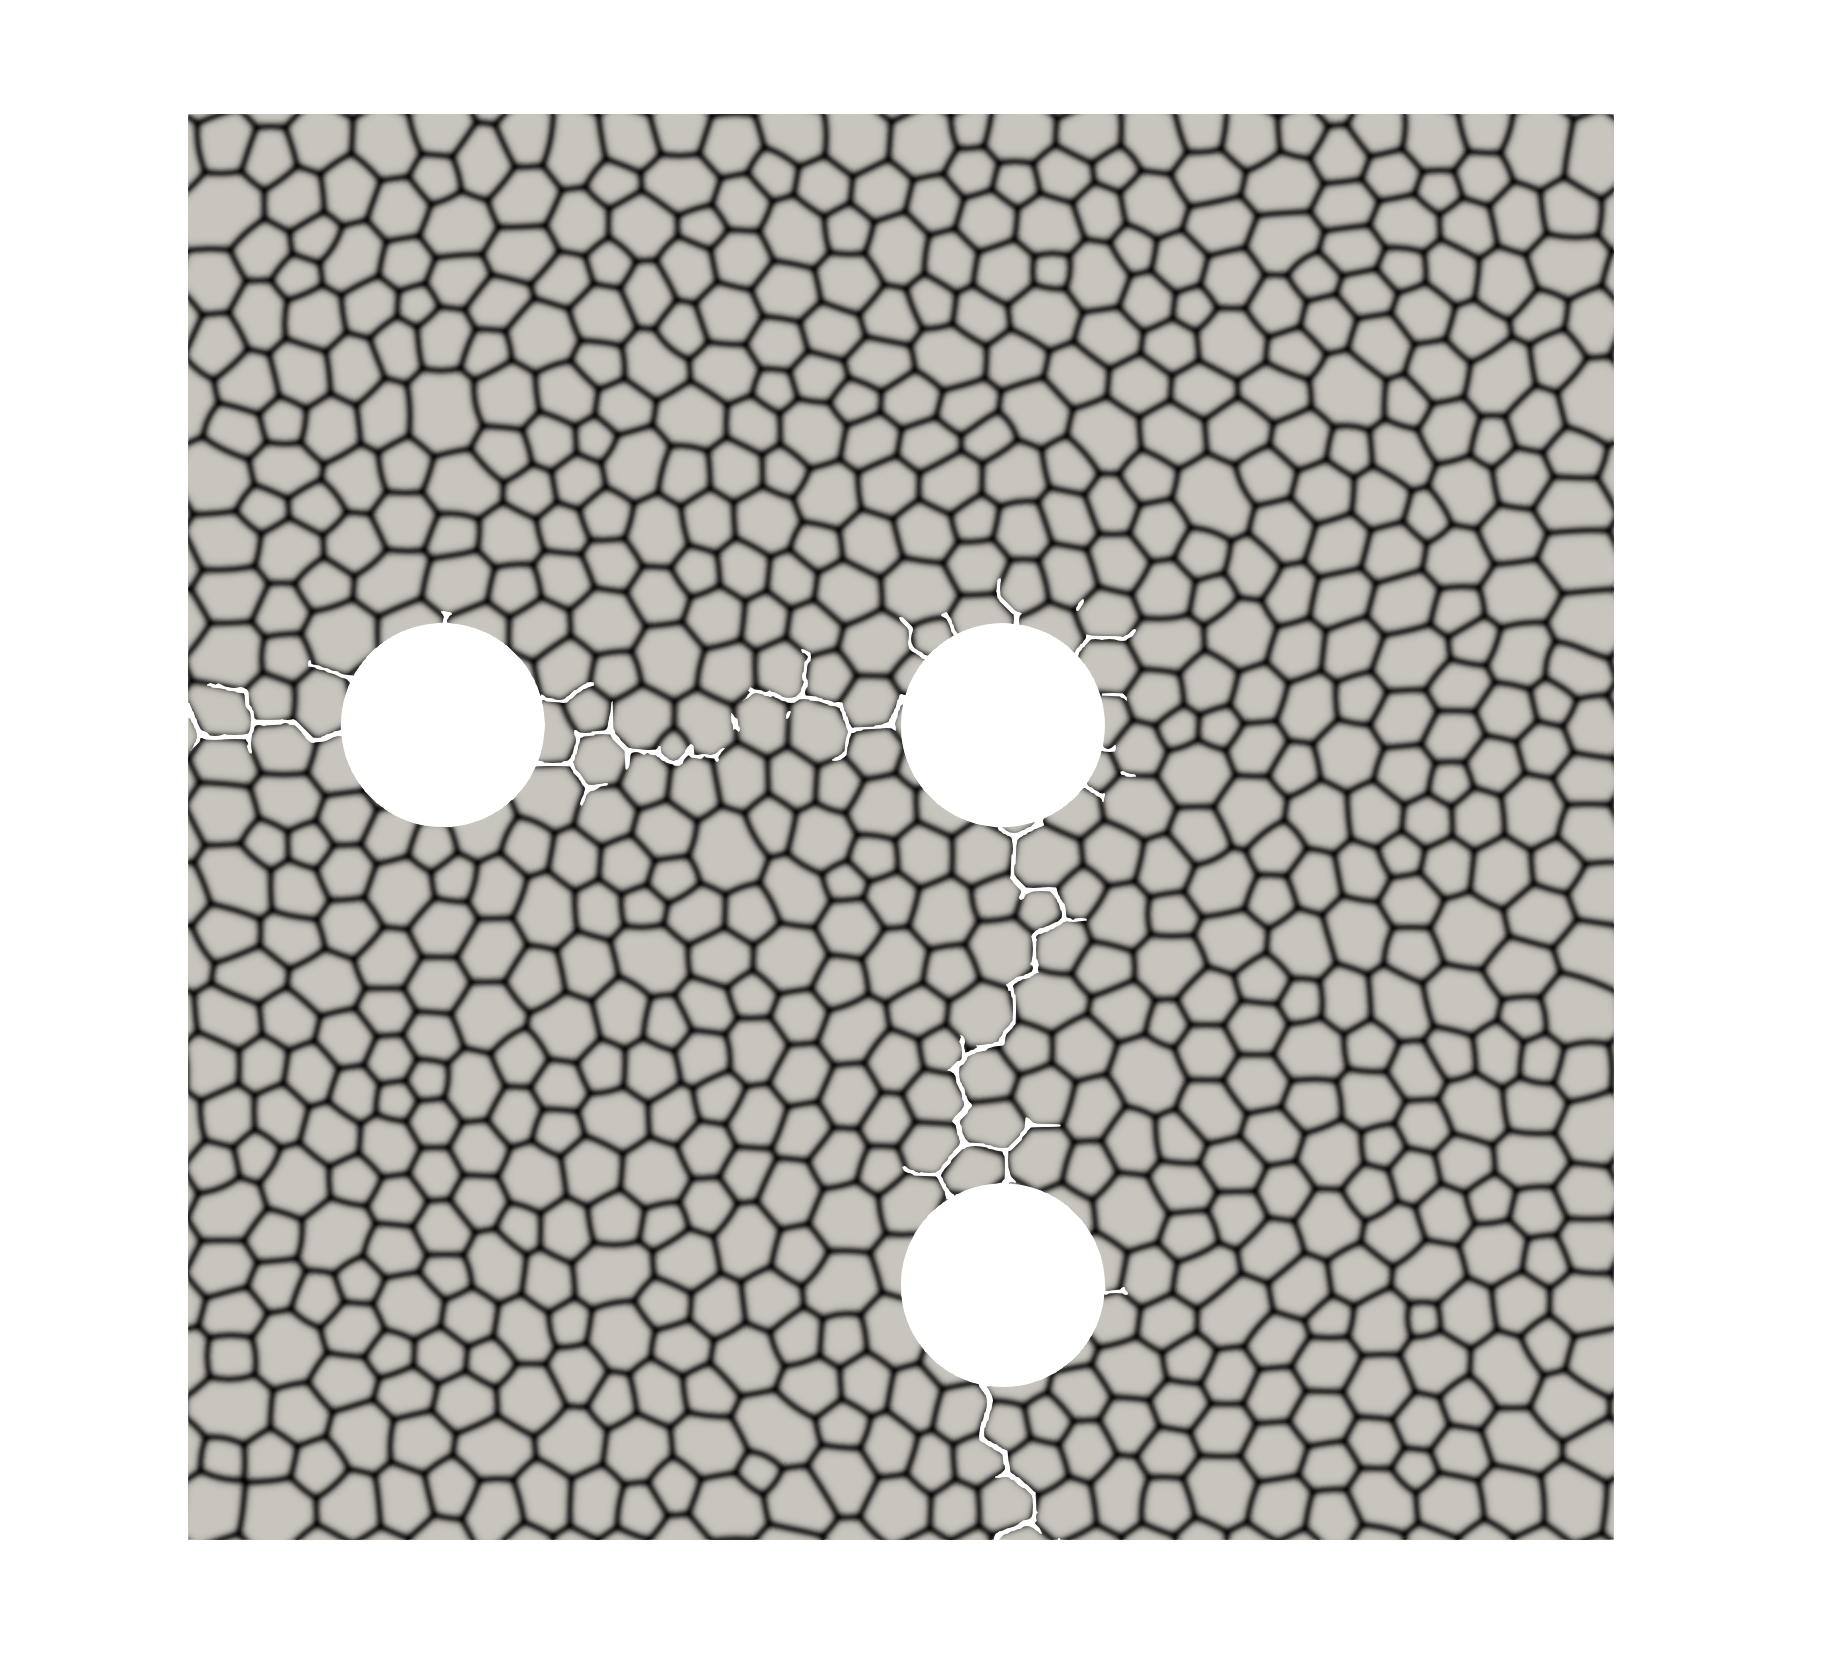
\includegraphics[width=\linewidth]{Chapter3/figures/three_bubbles_bnd}
    \caption{}
  \end{subfigure}
  \begin{subfigure}[t]{0.4\linewidth}
    \centering
    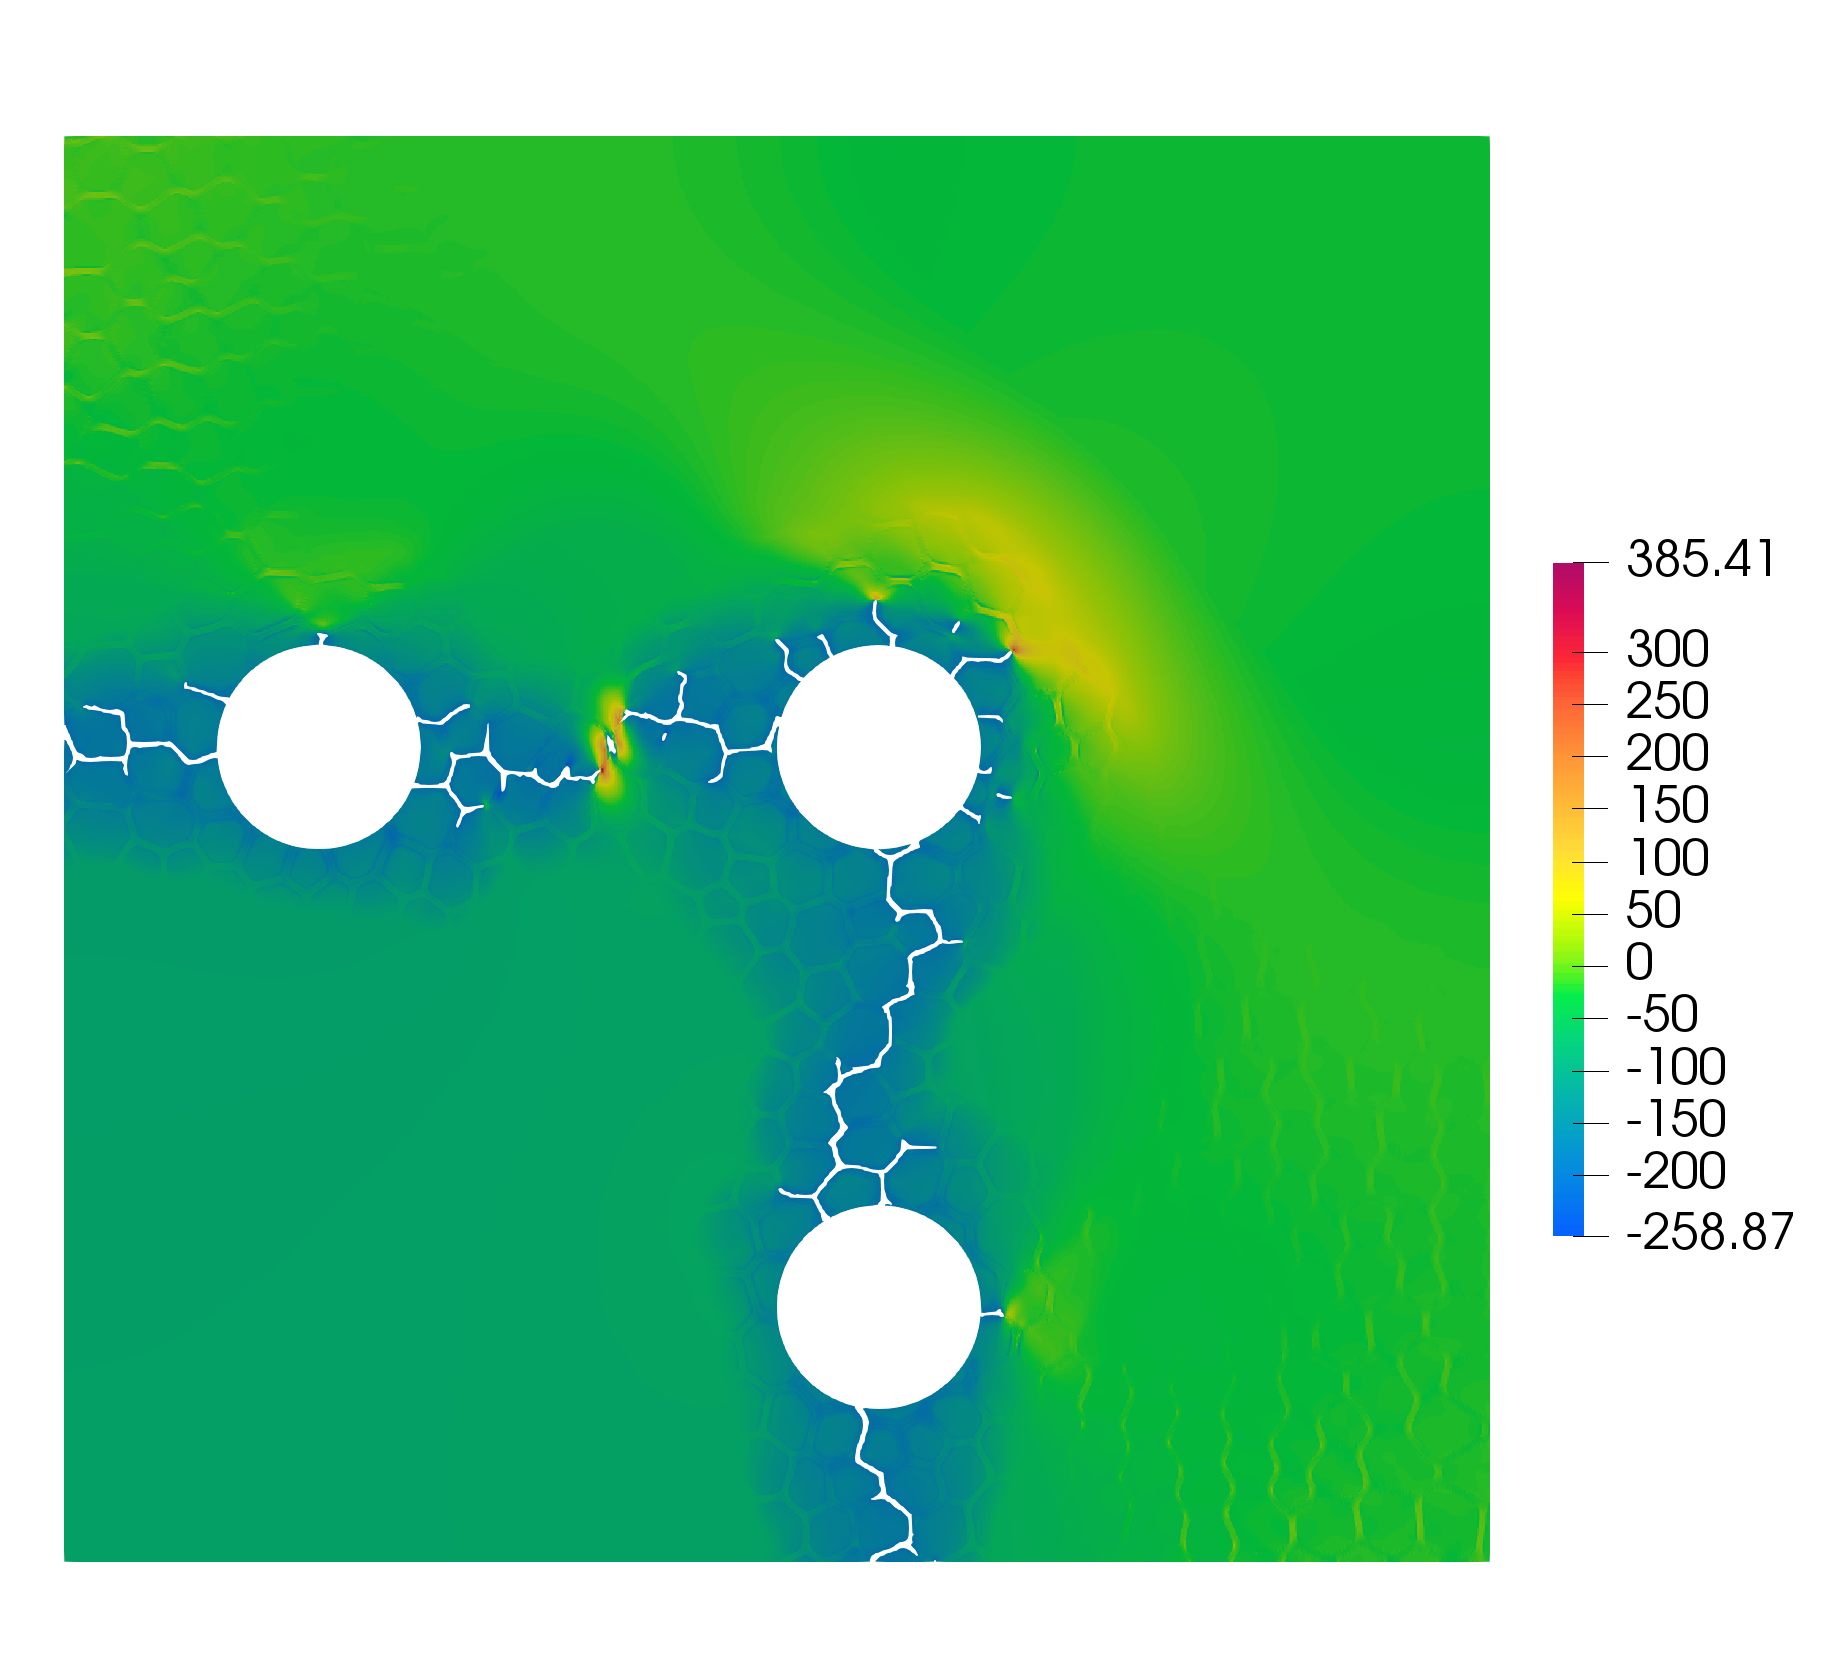
\includegraphics[width=\linewidth]{Chapter3/figures/three_bubbles_stress}
    \caption{}
  \end{subfigure}
  \caption{Results for (a-b) the two-bubble case and (c-d) the three-bubble case. (a, c) Crack paths superimposed on the voronoi structure. (b, d) Contour plot of the maximum principal stress.}
  \label{fig:compare_bubble_distribution}
\end{figure}

%%%%%%%%%%%%%%%%%%%%%%%%%%%%%%%%%%%%%%%%%%%%%%%%%%%%%%%%%%%%%%%%%%%%%%%%%%%%%%%%%%%%%%%%%%%
%%%%%%%%%%%%%%%%%%%%%%%%%%%%%%%%%%%%%%%%%%%%%%%%%%%%%%%%%%%%%%%%%%%%%%%%%%%%%%%%%%%%%%%%%%%
%%%%%%%%%%%%%%%%%%%%%%%%%%%%%%%%%%%%%%%%%%%%%%%%%%%%%%%%%%%%%%%%%%%%%%%%%%%%%%%%%%%%%%%%%%%
%%%%%%%%%%%%%%%%%%%%%%%%%%%%%%%%%%%%%%%%%%%%%%%%%%%%%%%%%%%%%%%%%%%%%%%%%%%%%%%%%%%%%%%%%%%
%%%%%%%%%%%%%%%%%%%%%%%%%%%%%%%%%%%%%%%%%%%%%%%%%%%%%%%%%%%%%%%%%%%%%%%%%%%%%%%%%%%%%%%%%%%
%%%%%%%%%%%%%%%%%%%%%%%%%%%%%%%%%%%%%%%%%%%%%%%%%%%%%%%%%%%%%%%%%%%%%%%%%%%%%%%%%%%%%%%%%%%
%%%%%%%%%%%%%%%%%%%%%%%%%%%%%%%%%%%%%%%%%%%%%%%%%%%%%%%%%%%%%%%%%%%%%%%%%%%%%%%%%%%%%%%%%%%
%%%%%%%%%%%%%%%%%%%%%%%%%%%%%%%%%%%%%%%%%%%%%%%%%%%%%%%%%%%%%%%%%%%%%%%%%%%%%%%%%%%%%%%%%%%
%%%%%%%%%%%%%%%%%%%%%%%%%%%%%%%%%%%%%%%%%%%%%%%%%%%%%%%%%%%%%%%%%%%%%%%%%%%%%%%%%%%%%%%%%%%
%%%%%%%%%%%%%%%%%%%%%%%%%%%%%%%%%%%%%%%%%%%%%%%%%%%%%%%%%%%%%%%%%%%%%%%%%%%%%%%%%%%%%%%%%%%
\subsubsection{Partial HBS}

Lastly, we incorporate defect evolution and recrystallization into the quasi-brittle fracture model. A phase-field model is used to simulate the defect evolution and the recrystallization behavior leading to HBS formation. A detailed description of the phase-field model is available in \cite{Aagesen2020}. The quasi-brittle fracture model is applied directly on the microstructure resulting from simulations of the HBS formation process. Considering the fact that fragmentation can be observed in partially recrystallized zones, we focus on the fracture behavior of partial HBS.
Three HBS at different recrystallization stages with $25\%$, $60\%$, and $100\%$ recrystallization fraction are considered. A linearly increasing gas pressure is applied. Results are shown in \Cref{fig:partial_hbs}. In all three cases, cracks nucleate at around 60 MPa, owing to their similar defect sizes. Crack nucleation locations vary among the three cases, as more grains form around the defect during recrystallization and their intersections with the defect become possible nucleation sites. Furthermore, recrystallization changes the grain morphology, leading to different crack paths.

\begin{figure}[htb!]
  \centering
  \begin{subfigure}[t]{0.4\linewidth}
    \centering
    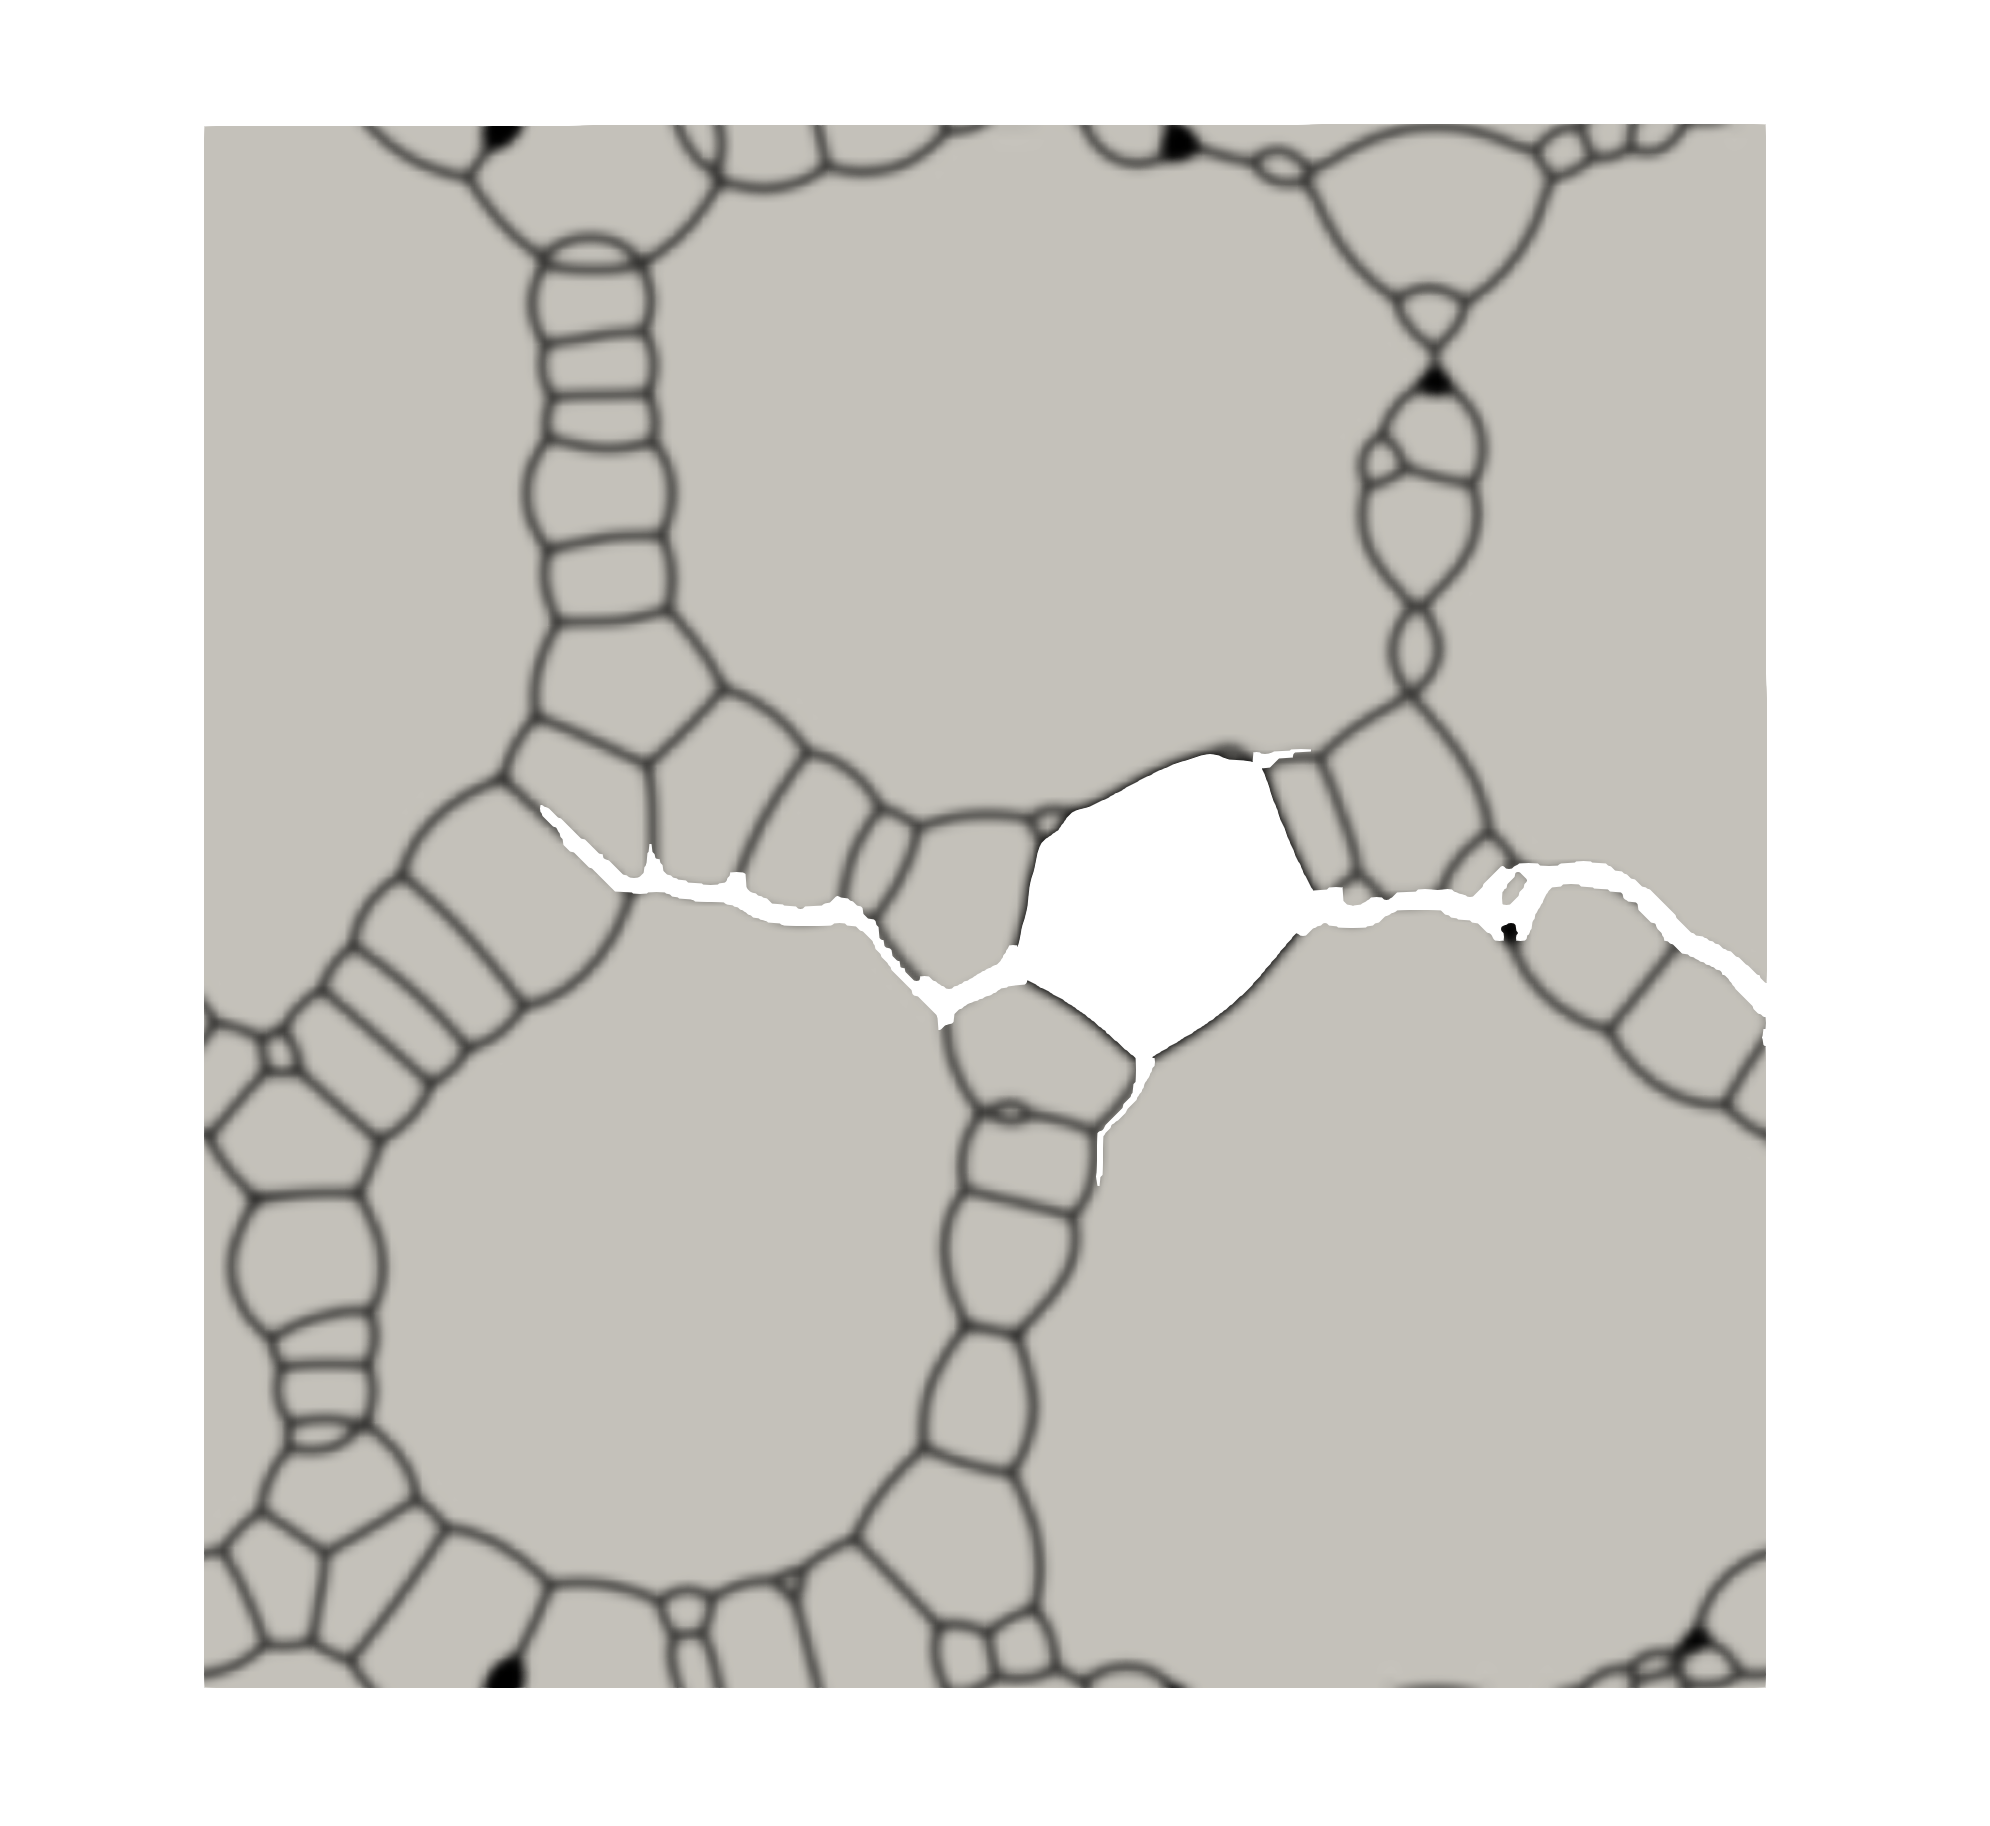
\includegraphics[width=\linewidth]{Chapter3/figures/partial_hbs_1}
    \caption{}
  \end{subfigure}
  \begin{subfigure}[t]{0.4\linewidth}
    \centering
    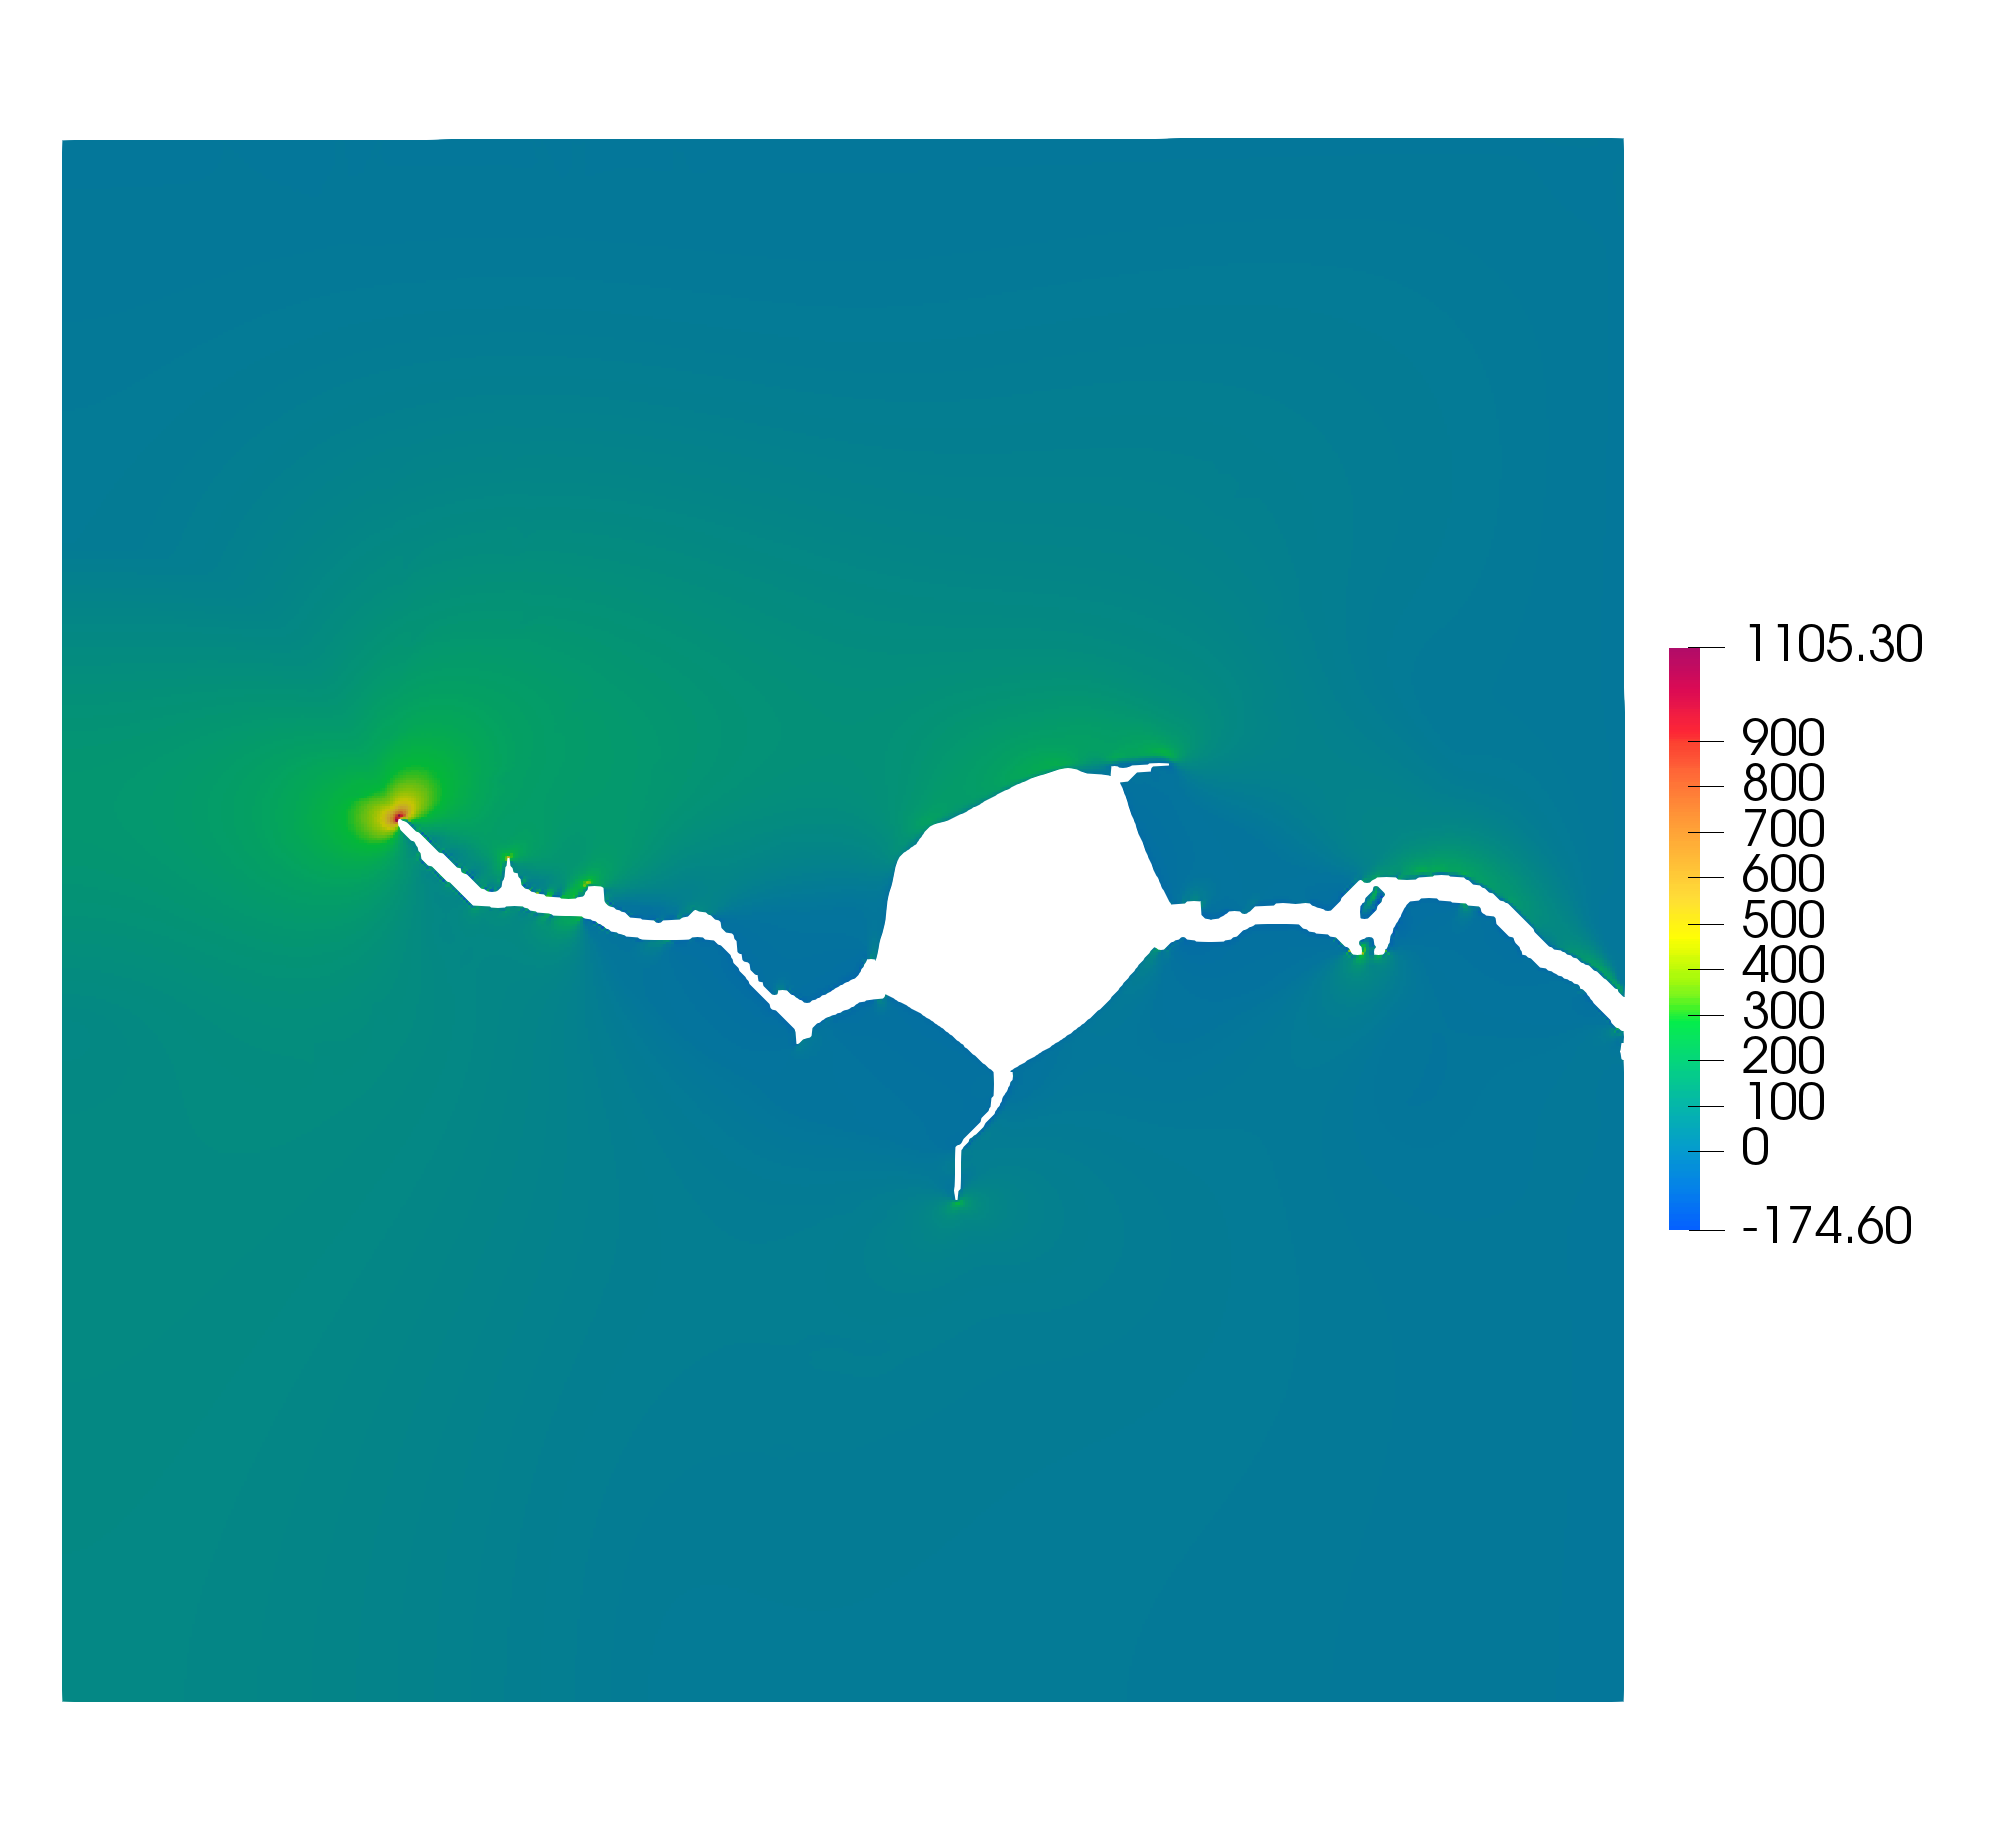
\includegraphics[width=\linewidth]{Chapter3/figures/partial_hbs_1_stress}
    \caption{}
  \end{subfigure}\\
  \begin{subfigure}[t]{0.4\linewidth}
    \centering
    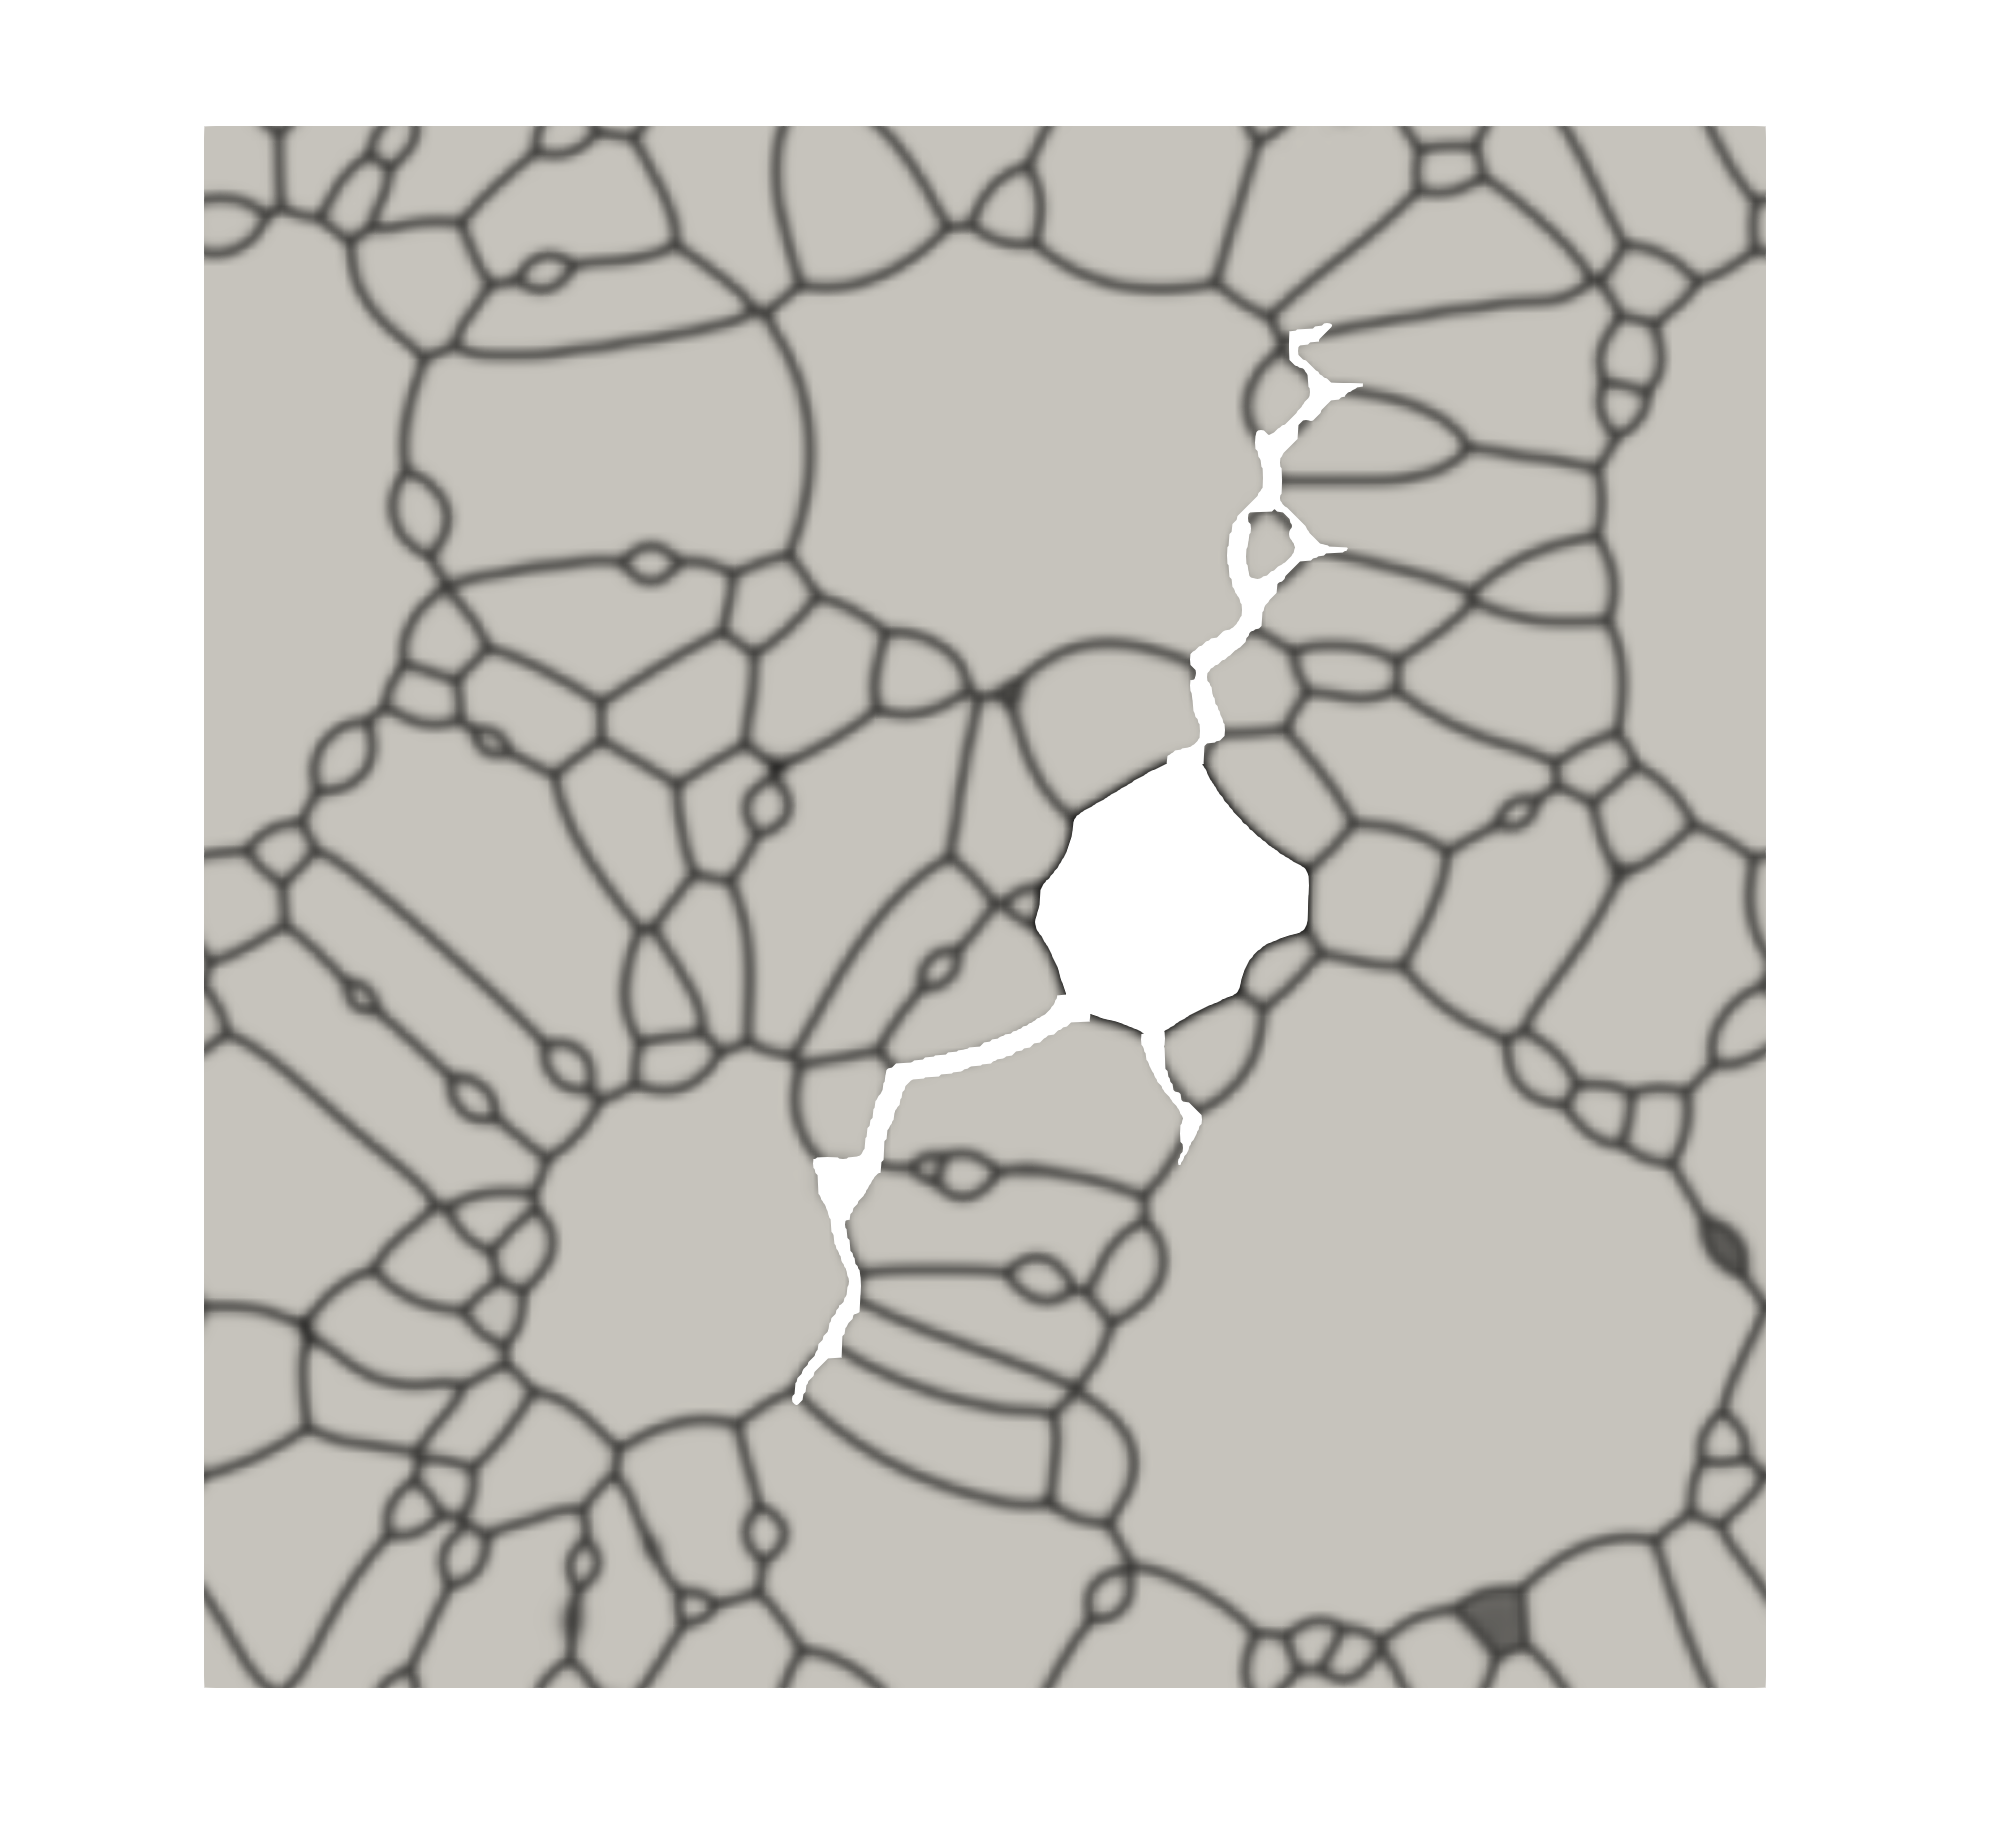
\includegraphics[width=\linewidth]{Chapter3/figures/partial_hbs_2}
    \caption{}
  \end{subfigure}
  \begin{subfigure}[t]{0.4\linewidth}
    \centering
    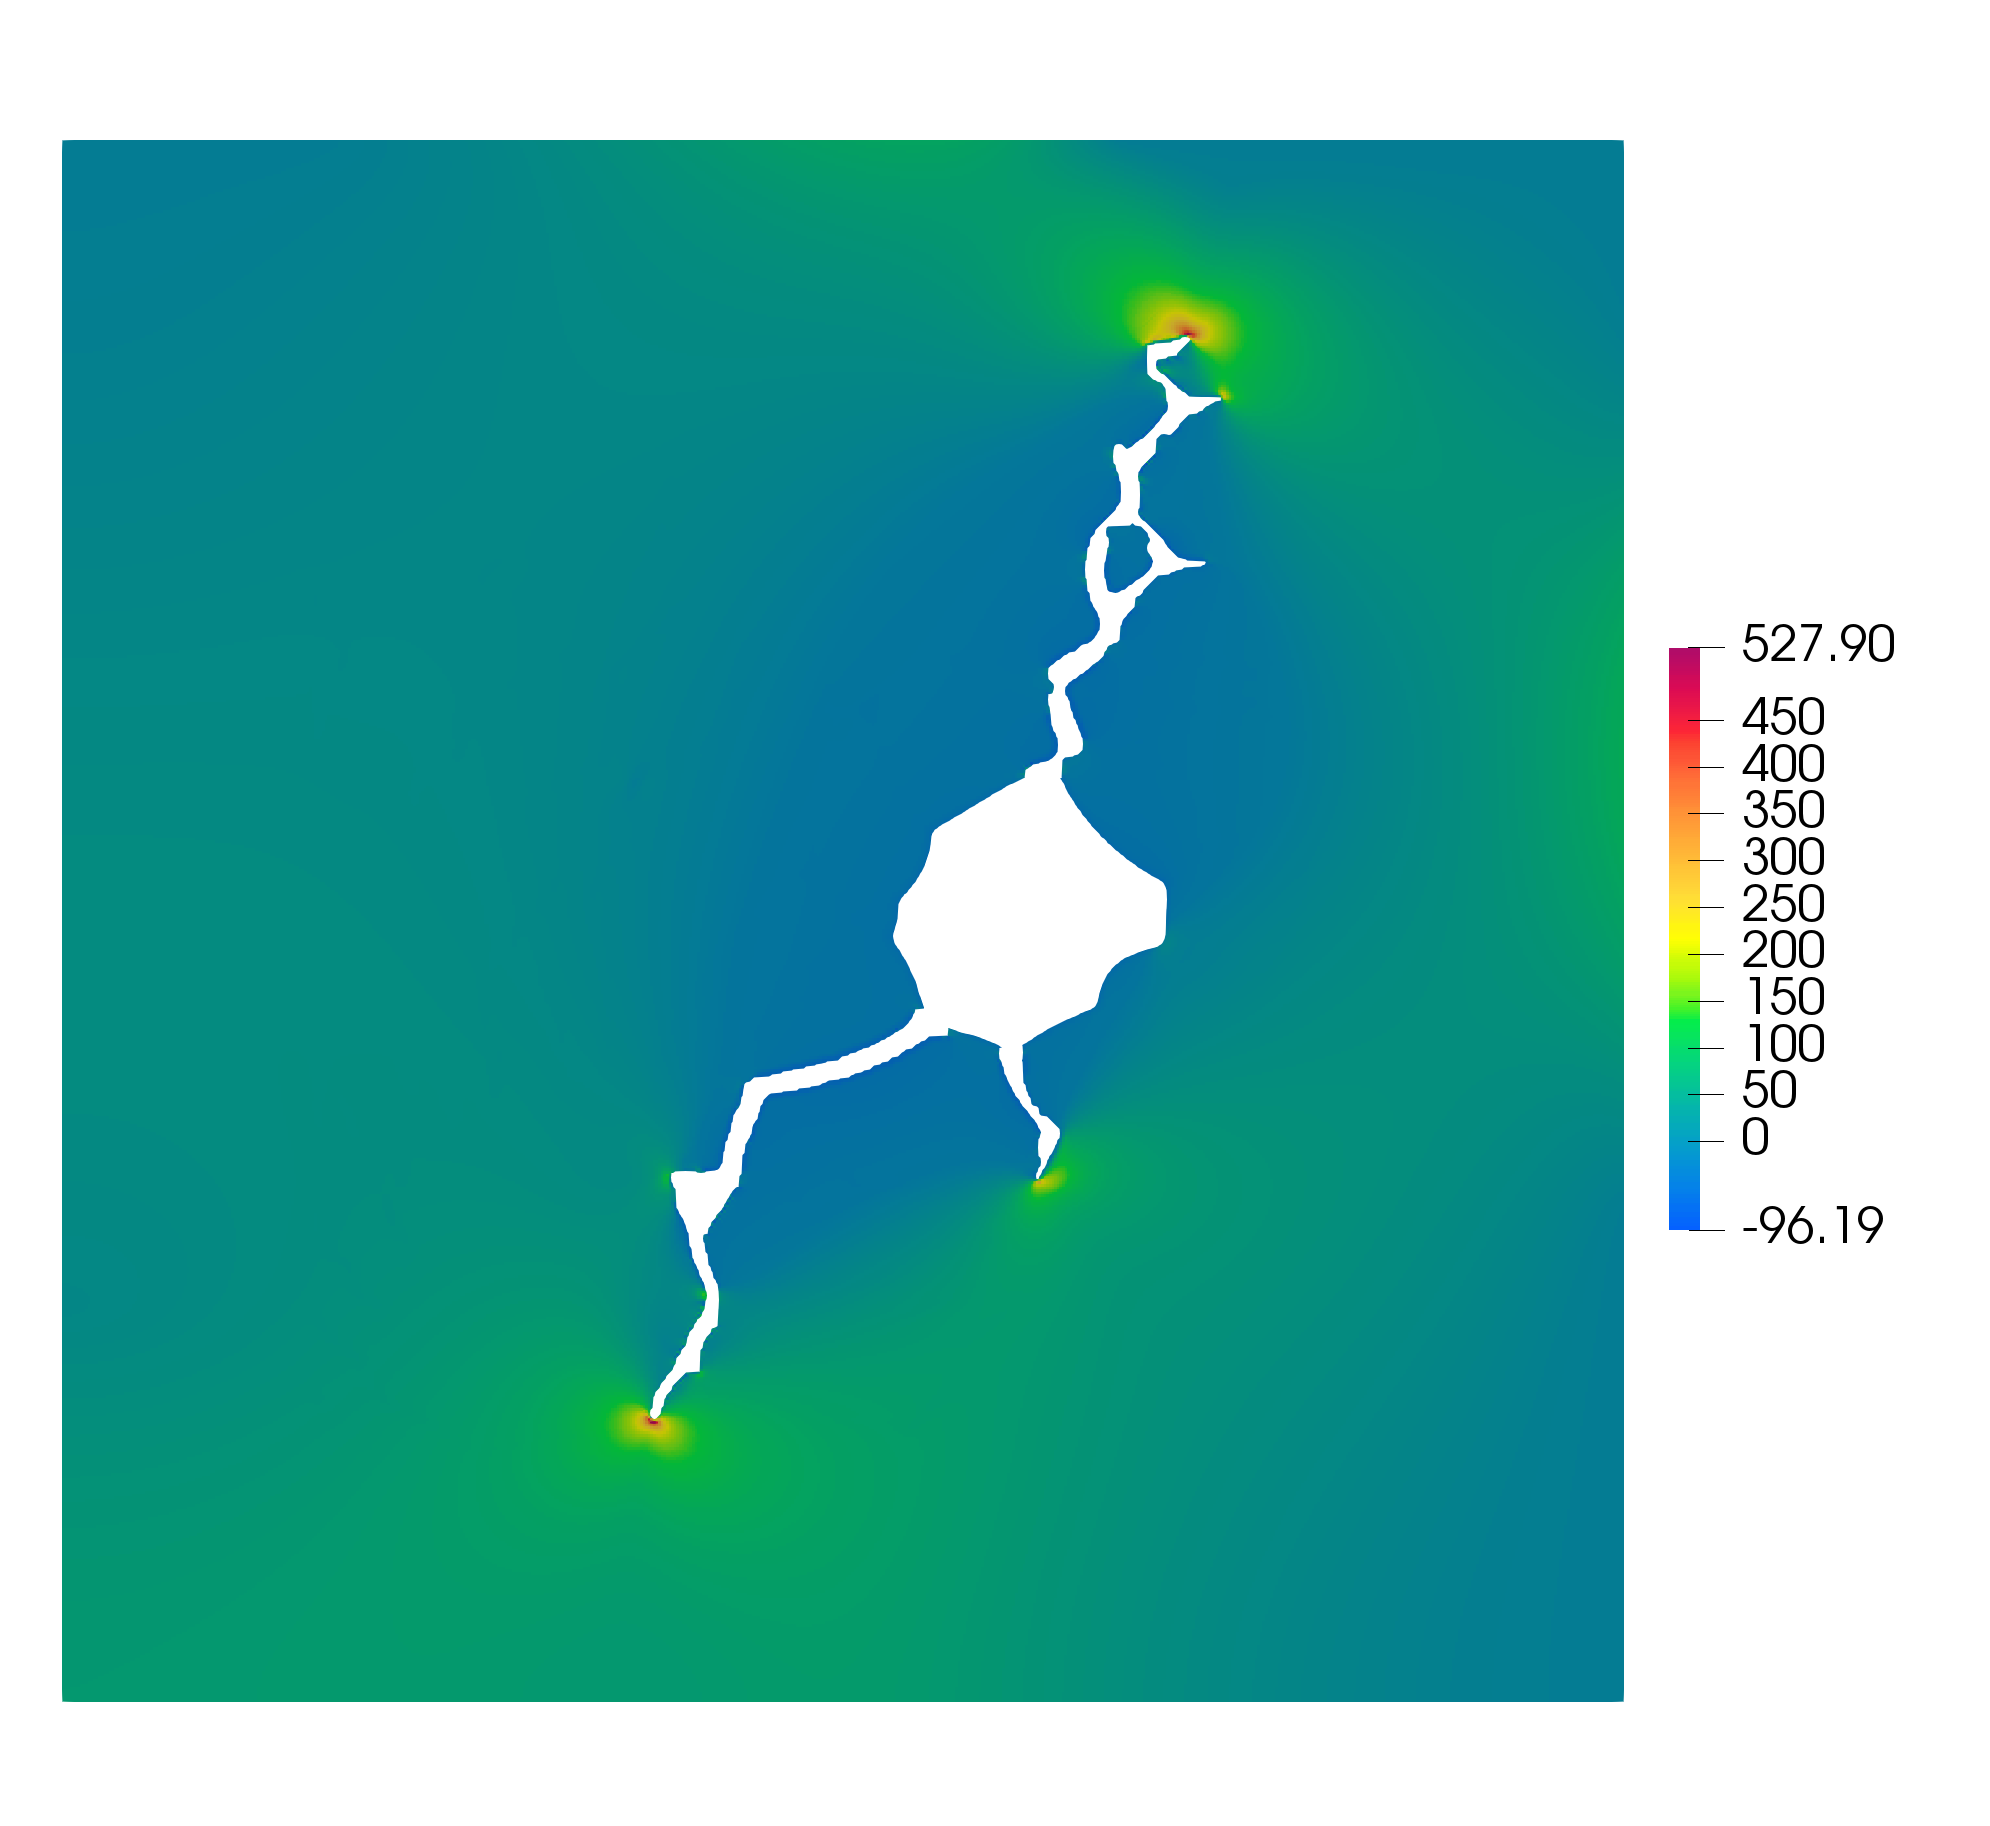
\includegraphics[width=\linewidth]{Chapter3/figures/partial_hbs_2_stress}
    \caption{}
  \end{subfigure}\\
  \begin{subfigure}[t]{0.4\linewidth}
    \centering
    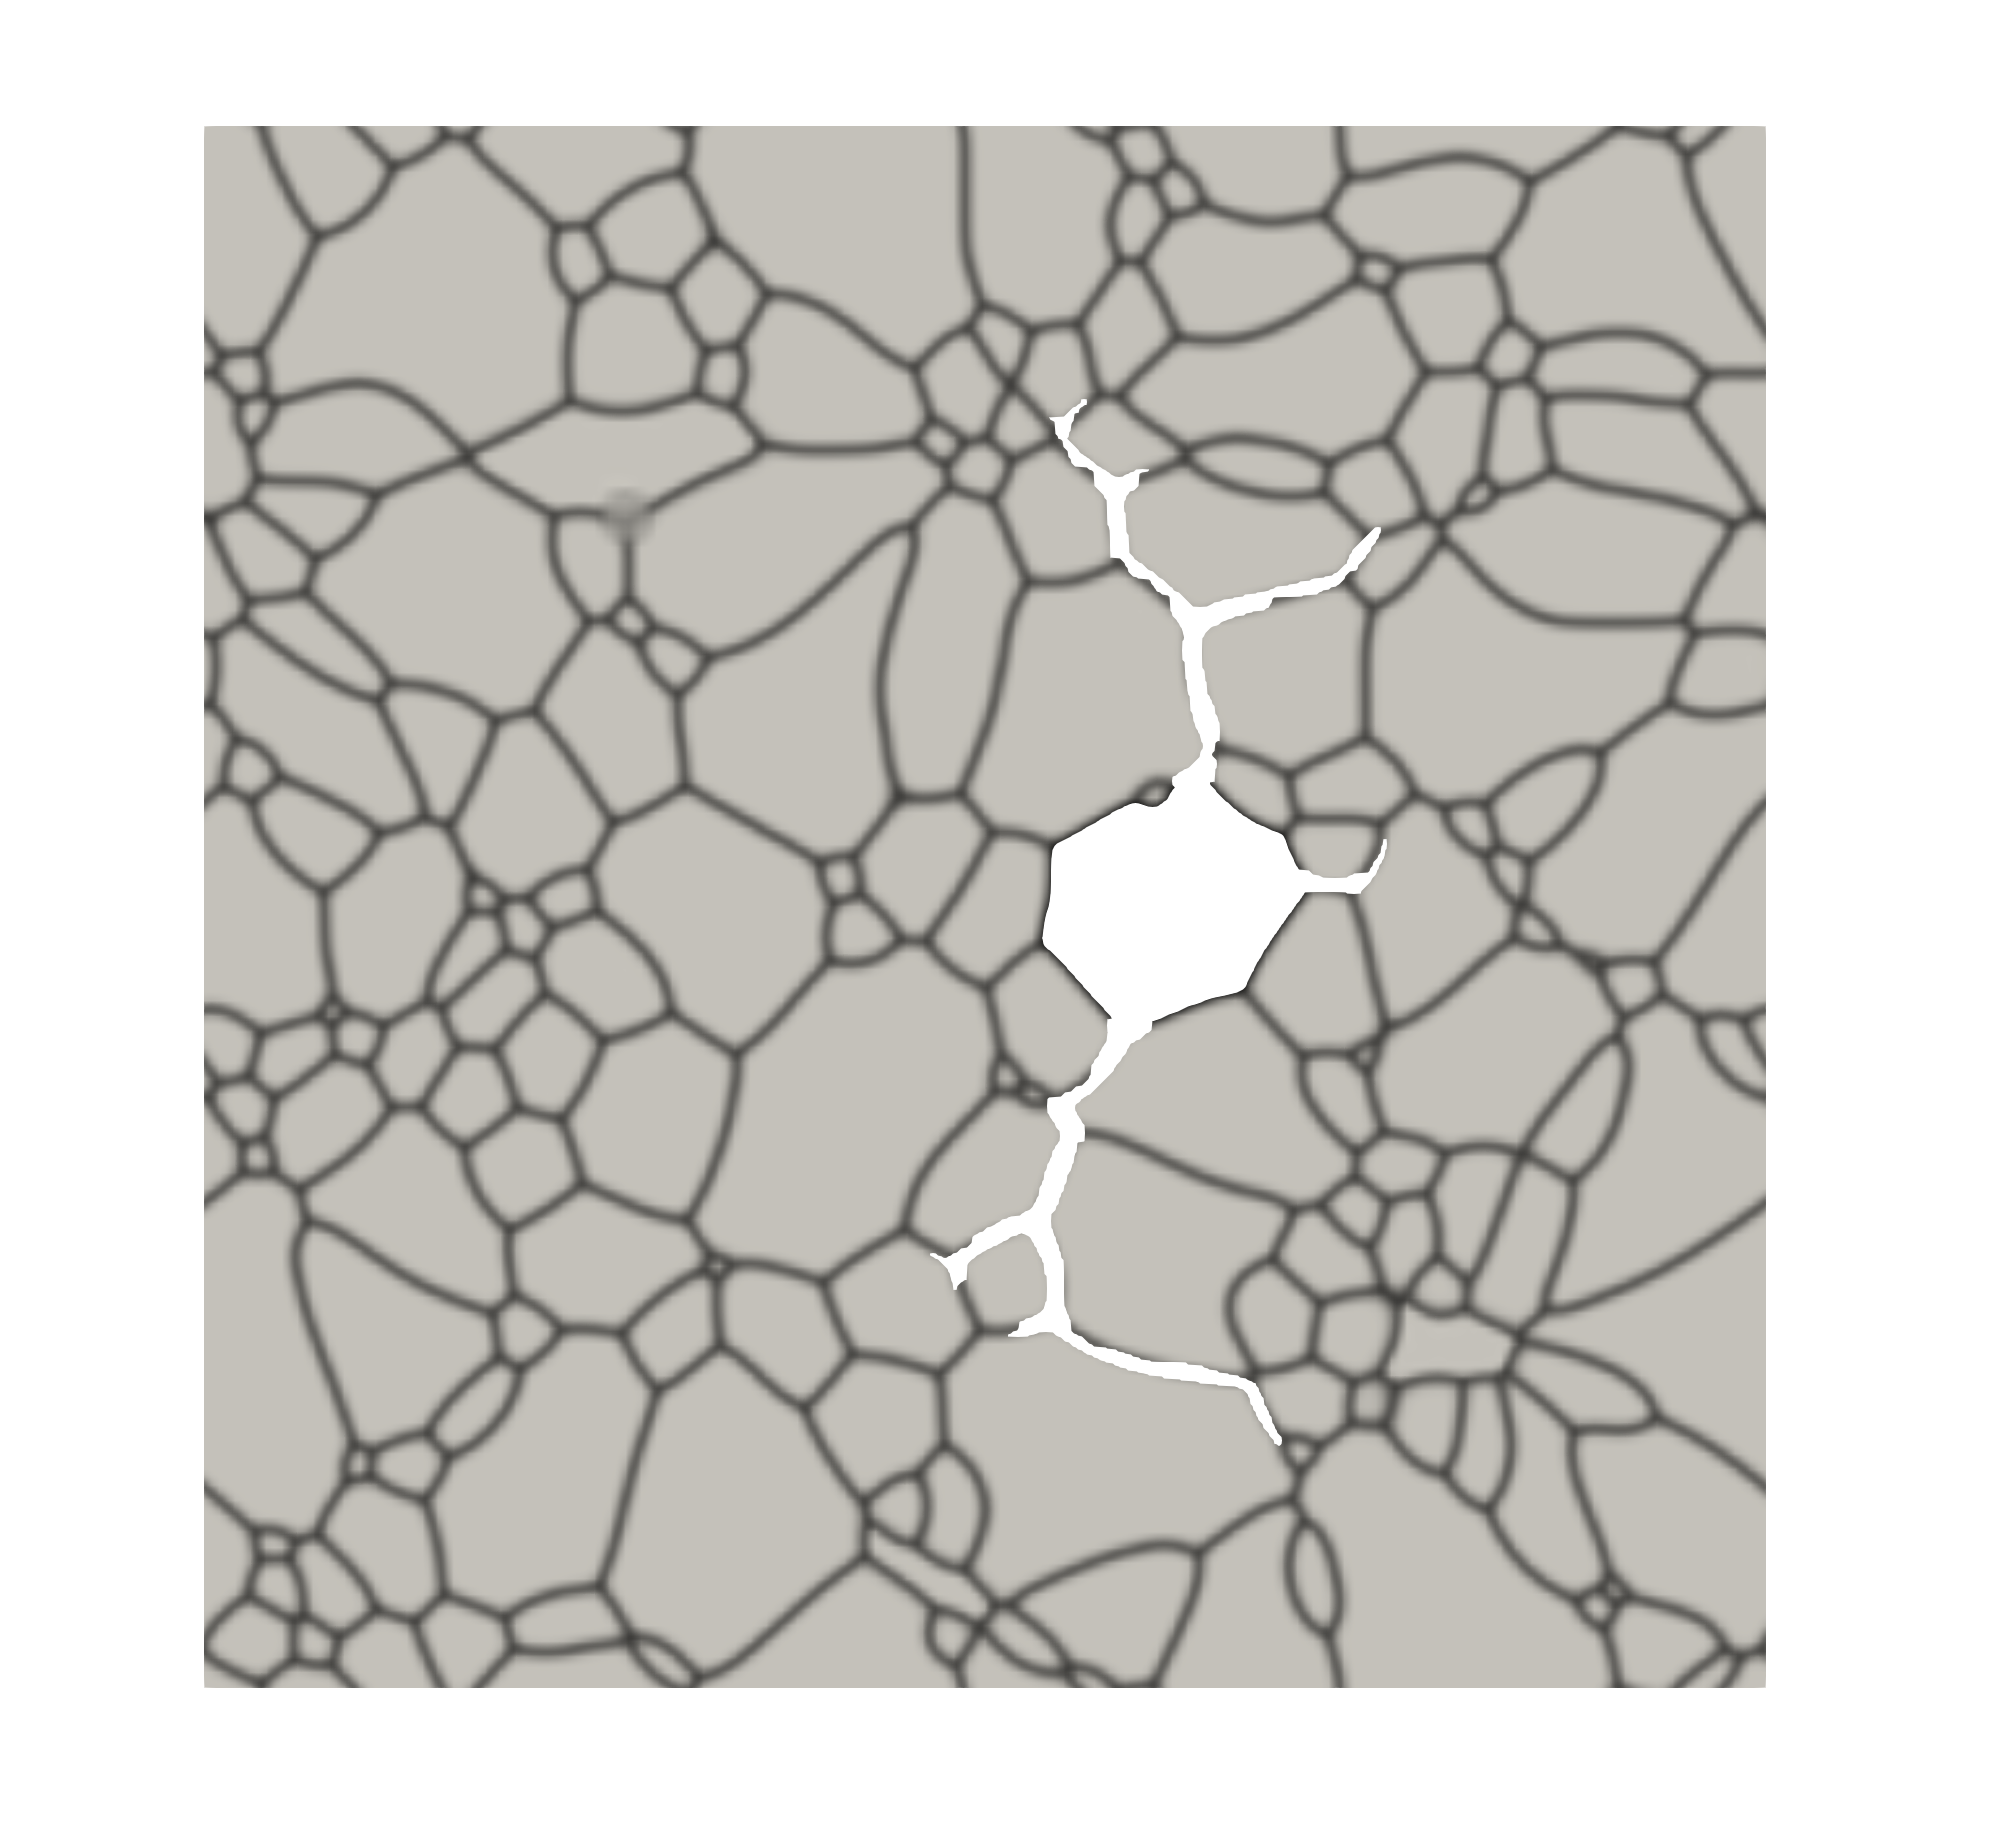
\includegraphics[width=\linewidth]{Chapter3/figures/partial_hbs_3}
    \caption{}
  \end{subfigure}
  \begin{subfigure}[t]{0.4\linewidth}
    \centering
    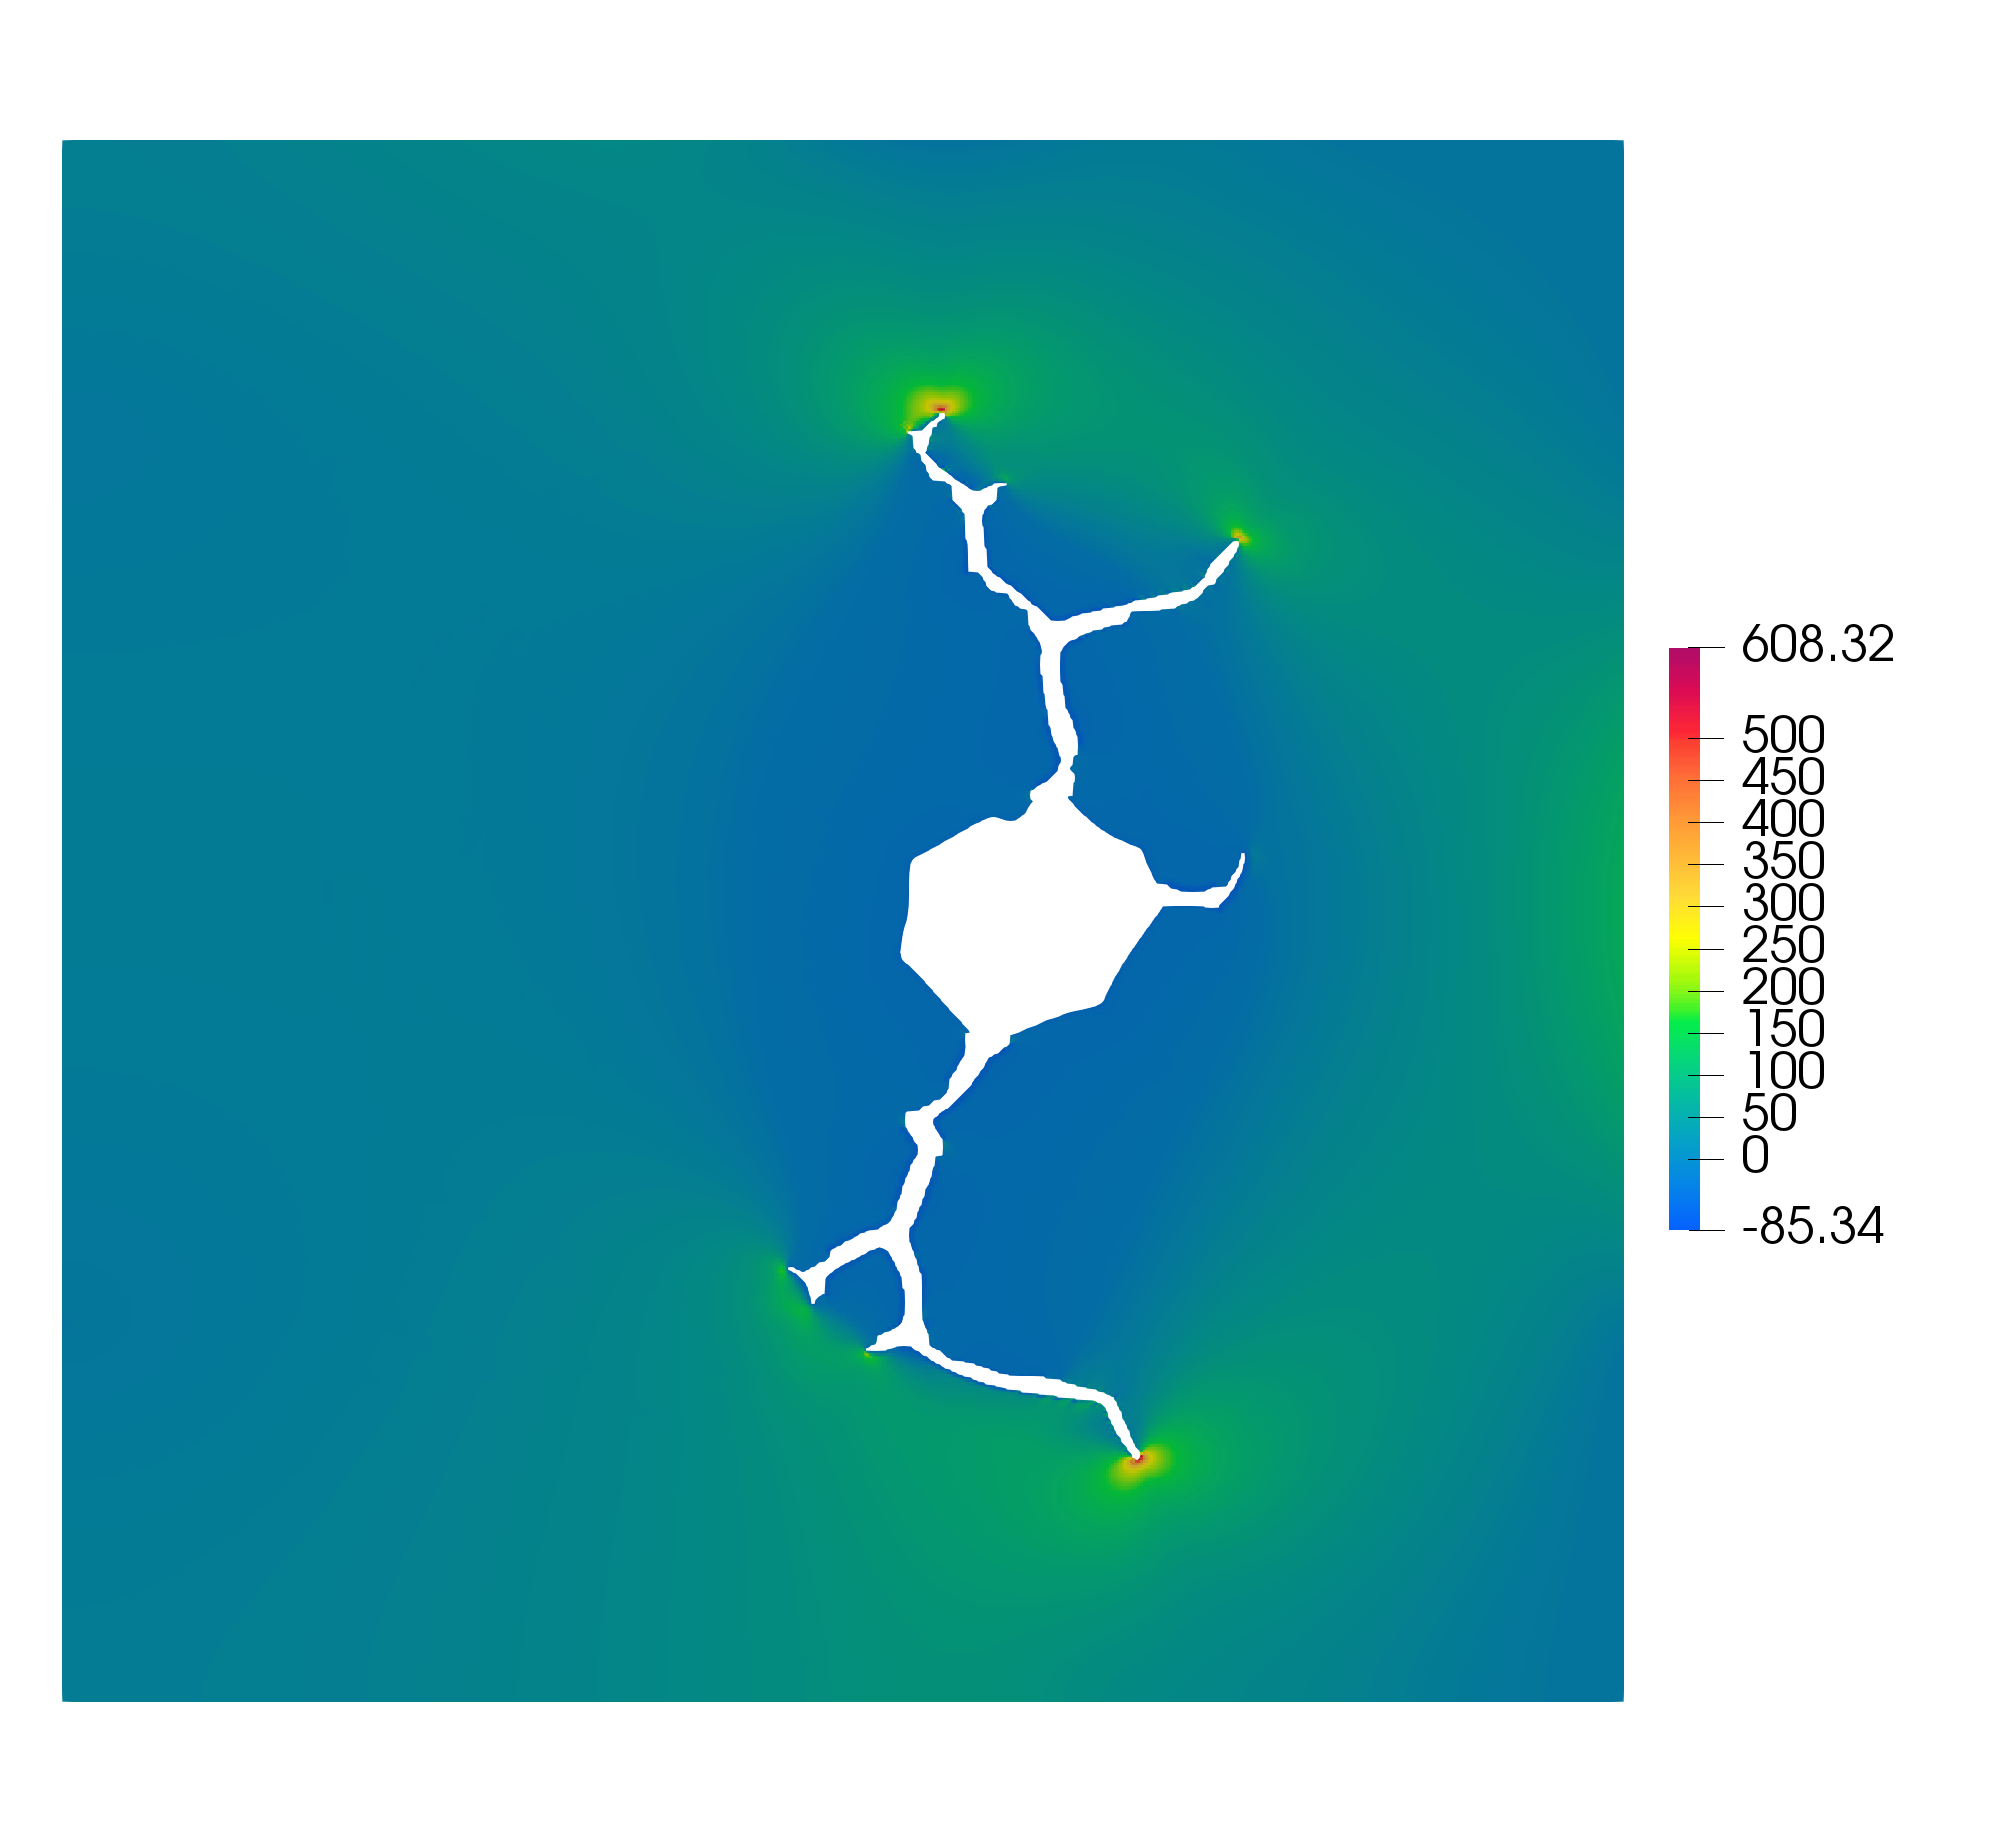
\includegraphics[width=\linewidth]{Chapter3/figures/partial_hbs_3_stress}
    \caption{}
  \end{subfigure}
  \caption{ (a, c, e) Crack paths superimposed on the microstructure and (b, d, f) contour plots of the maximum principal stress assuming different recrystallization stages: (a-b) $25\%$ recrystallization, (c-d) $60\%$ recrystallization, (e-f) $100\%$ recrystallization. }
  \label{fig:partial_hbs}
\end{figure}
